\documentclass[a4paper,12pt]{article}
\usepackage{listings}
\usepackage{xcolor}
\usepackage{graphics}
\usepackage{graphicx}
\usepackage[frenchb]{babel}
\usepackage{framed}
\usepackage{amsmath}
\usepackage{amssymb}
\usepackage{hyperref}

%\usepackage{fancyhdr}
%\setlength{\headheight}{55.2pt}
%\setlength{\headwidth}{\textwidth}
%\fancyfoot[L]{
\includegraphics[height=0.4in]{licence-by-nc-sa.png}}
%\pagestyle{fancyplain}

\usepackage[utf8]{inputenc}

\usepackage{verbatim}
%pour les algorithmes
\usepackage{algorithm}
\usepackage{algpseudocode} 

\definecolor{codegreen}{rgb}{0,0.6,0}
\definecolor{codegray}{rgb}{0.5,0.5,0.5}
\definecolor{codepurple}{rgb}{0.58,0,0.82}
\definecolor{backcolour}{rgb}{0.95,0.95,0.92}

\usepackage[a4paper,left=2cm,right=2cm,top=2cm,bottom=2cm]{geometry}

%backgroundcolor=\color{backcolour}

\lstdefinestyle{mystyle}{
    backgroundcolor=\color{white},   
    commentstyle=\color{codegreen},
    keywordstyle=\color{magenta},
    numberstyle=\tiny\color{codegray},
    stringstyle=\color{codepurple},
    basicstyle=\ttfamily\footnotesize,
    breakatwhitespace=false,         
    breaklines=true,                 
    captionpos=b,                    
    keepspaces=true,                 
    numbers=left,                    
    numbersep=5pt,                  
    showspaces=false,                
    showstringspaces=false,
    showtabs=false,                  
    tabsize=2,
    caption=\lstname                   % show the filename of files included with \lstinputlisting; also try caption instead of title	
}

\lstset{style=mystyle}
\author{A. Aoufi et BOUSSEJRA Amir}
\title{Introduction express \`a la programmation Python}

\date{12 Septembre 2025}
\begin{document}
\maketitle
\begin{center}

\includegraphics[height=0.8in]{./png/licence-by-nc-sa.png}
\end{center}
\clearpage
\tableofcontents

\clearpage
\section{Introduction à Python}
\subsection{G\'en\'eralit\'es}
\begin{enumerate}
\item langage orient\'e objet ( i.e. fusion variables et m\'ethodes ), interpr\'et\'e ( i.e. ex\'ecution ligne par ligne. Relativement lent mais peut \^etre  acc\'el\'er\'e notablement avec les  biblioth\`eques ad\'equates.
\item bas\'e sur le langage C mis au point en 1972 par Dennis Ritchie et Ken Thompson des laboratoires Bell.
\item cr\'e\'e en 1985 par Guido Van Rossum.
\item les scripts ou programmes sont sauvegard\'es sous format ASCII dans un fichier d'extension .py. Exemple program.py contient une suite d'instructions.
\end{enumerate}
\subsection{Bibliographie}
Les ouvrages suivants ne sont pas obligatoires mais permettent de plus approfondir les notions pr\'esent\'ees succintement dans ce document.
\begin{enumerate}
\item Prépabac NSI 1re générale (spécialité) : nouveau programme de Première : 978-2401094932 de Céline Adobet, Guillaume Connan, Gérard Rozsavolgyi, Laurent Signac. Ed Hatier.
\begin{figure}[h]
\begin{center}

\includegraphics[height=6cm]{./png/hatier-python-1ere}
\end{center}
\end{figure}
\item Prépabac NSI Tle générale (spécialité) - Bac 2024: nouveau programme de Terminale: 978-2401094925 : 
de Guillaume Connan, Vojislav Petrov, Gérard Rozsavolgyi, Laurent Signac. Ed Hatier.
\begin{figure}[h]
\begin{center}

\includegraphics[height=6cm]{./png/hatier-python-term}
\end{center}
\end{figure}
\end{enumerate}
\clearpage

\subsection{Utiliser Python avec Google Colab (recommandé)}

Google Colab est une plateforme en ligne gratuite permettant de développer et d’exécuter des scripts Python directement dans le navigateur, sans besoin d’installation locale ni de configuration complexe. Pour accéder à Google Colab, il suffit de posséder un compte Google et de se rendre à l’adresse \url{https://colab.research.google.com/}. L’interface propose la création de notebooks interactifs (.ipynb), adaptés au développement et à la présentation de travaux en Python sommaires.

\begin{figure}[h]
\begin{center}
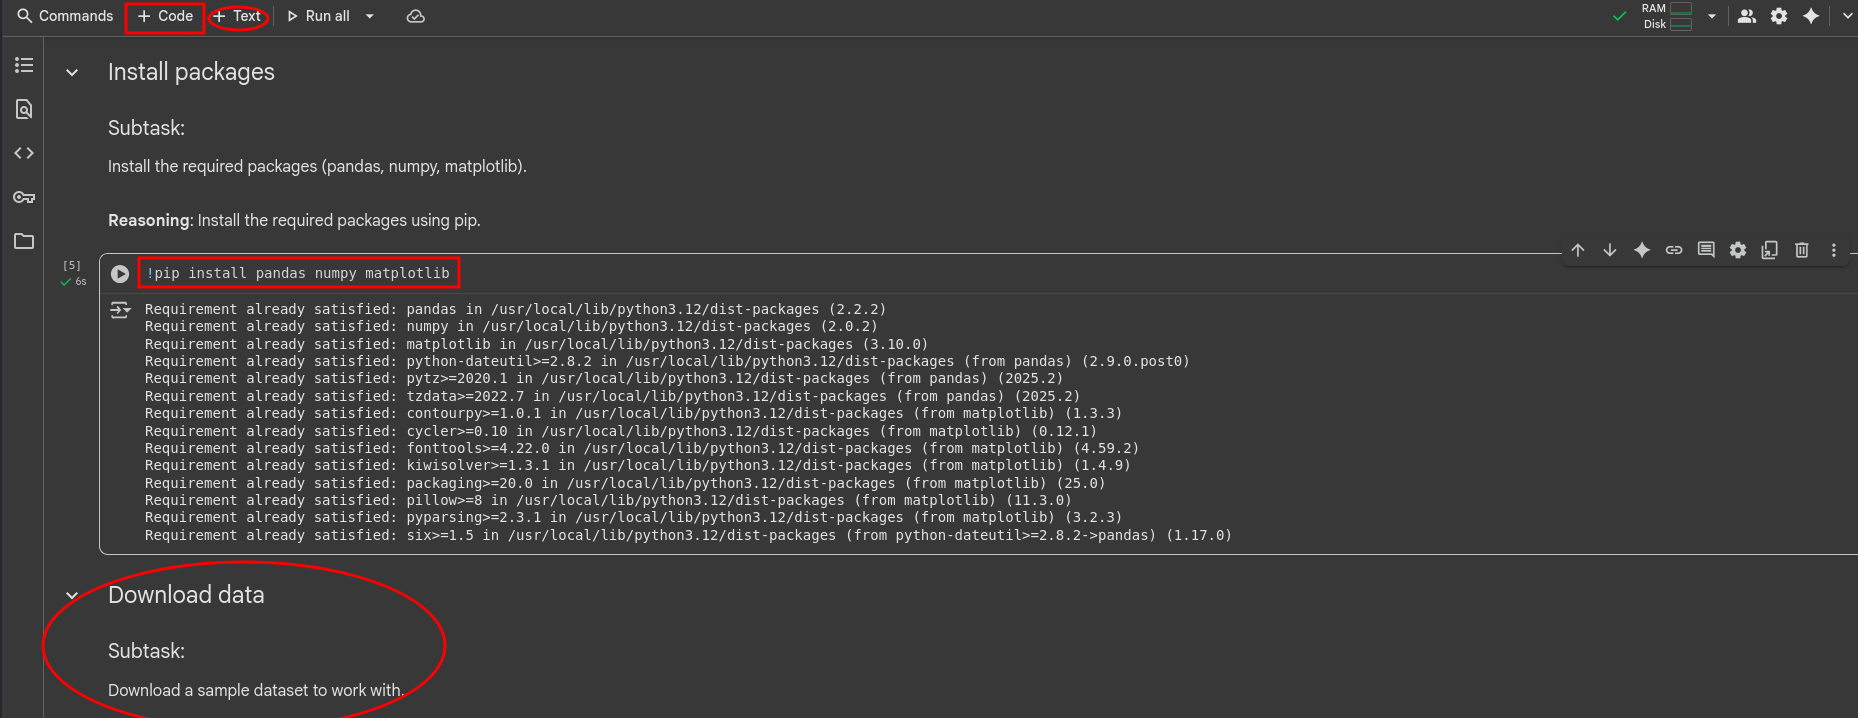
\includegraphics[width=10cm]{./png/google-colab-ui}
\end{center}
\caption{Interface de démarrage de Google Colab.}
\end{figure}

\subsection{Installation de packages Python dans Colab}

Contrairement à un environnement local, l’installation de packages dans Colab s’effectue facilement via la commande \texttt{!pip install} en début de cellule, par exemple :

\begin{verbatim}
!pip install numpy pandas matplotlib scikit-learn
\end{verbatim}

Cette organisation permet de bénéficier rapidement et facilement des outils scientifiques Python (Numpy, pandas, matplotlib, etc.), sans manipulation complexe sur le poste local. Travail collaboratif, partage immédiat et simplicité d’accès sont les avantages majeurs de Google Colab pour le développement Python moderne.

Pour l'utilisation en détail (ouverture de fichiers de votre ordinateur, partage de fichiers, autres problèmes). Je n'ai pas de doute que vous trouverez facilement seul ! L'interface est très intuitive.

\clearpage
\subsection{Installation python avec anaconda (non recommandé)}
Utiliser le lien suivant: \url{https://www.anaconda.com/download/}. S\'electionner la version compatible avec le syst\`eme d'exploitation.
\begin{figure}[h]
\begin{center}

\includegraphics[width=10cm]{./png/anaconda-install}
\end{center}
\caption{Choix de la version de l'installateur anaconda.}
\end{figure}
Deux m\'ethodes sont disponibles pour l'ex\'ecution d'un script python
\begin{enumerate}
\item spyder : d\'eveloppement du script python (.py) , debuggage et analyse du contenu des variables. 
\item Jupyter notebook (.ipynb), ex\'ecution par bloc d'instructions et sortie au format pdf du travail effectué.
\end{enumerate}



%--spyder
\clearpage
\subsection{Environnement Spyder (non recommandé)}
Cet environnement sera utilisé pour la mise au point des scripts python.
Afin d'y acc\'eder, il faut
\begin{enumerate}
\item double cliquer sur l'ic\^one anaconda navigator
\begin{figure}[h]
\begin{center}

\includegraphics[height=2cm]{./png/anaconda-navigator}
\end{center}
\end{figure}
\item Cliquer sous l'ic\^one relative \`a Spyder : appuyer sur launch
\begin{figure}[h]
\begin{center}

\includegraphics[height=8cm]{./png/menu-anaconda-navigator}
\end{center}
\end{figure}
\item L'environnement Spyder appara\^it alors.
\begin{figure}[h]
\begin{center}
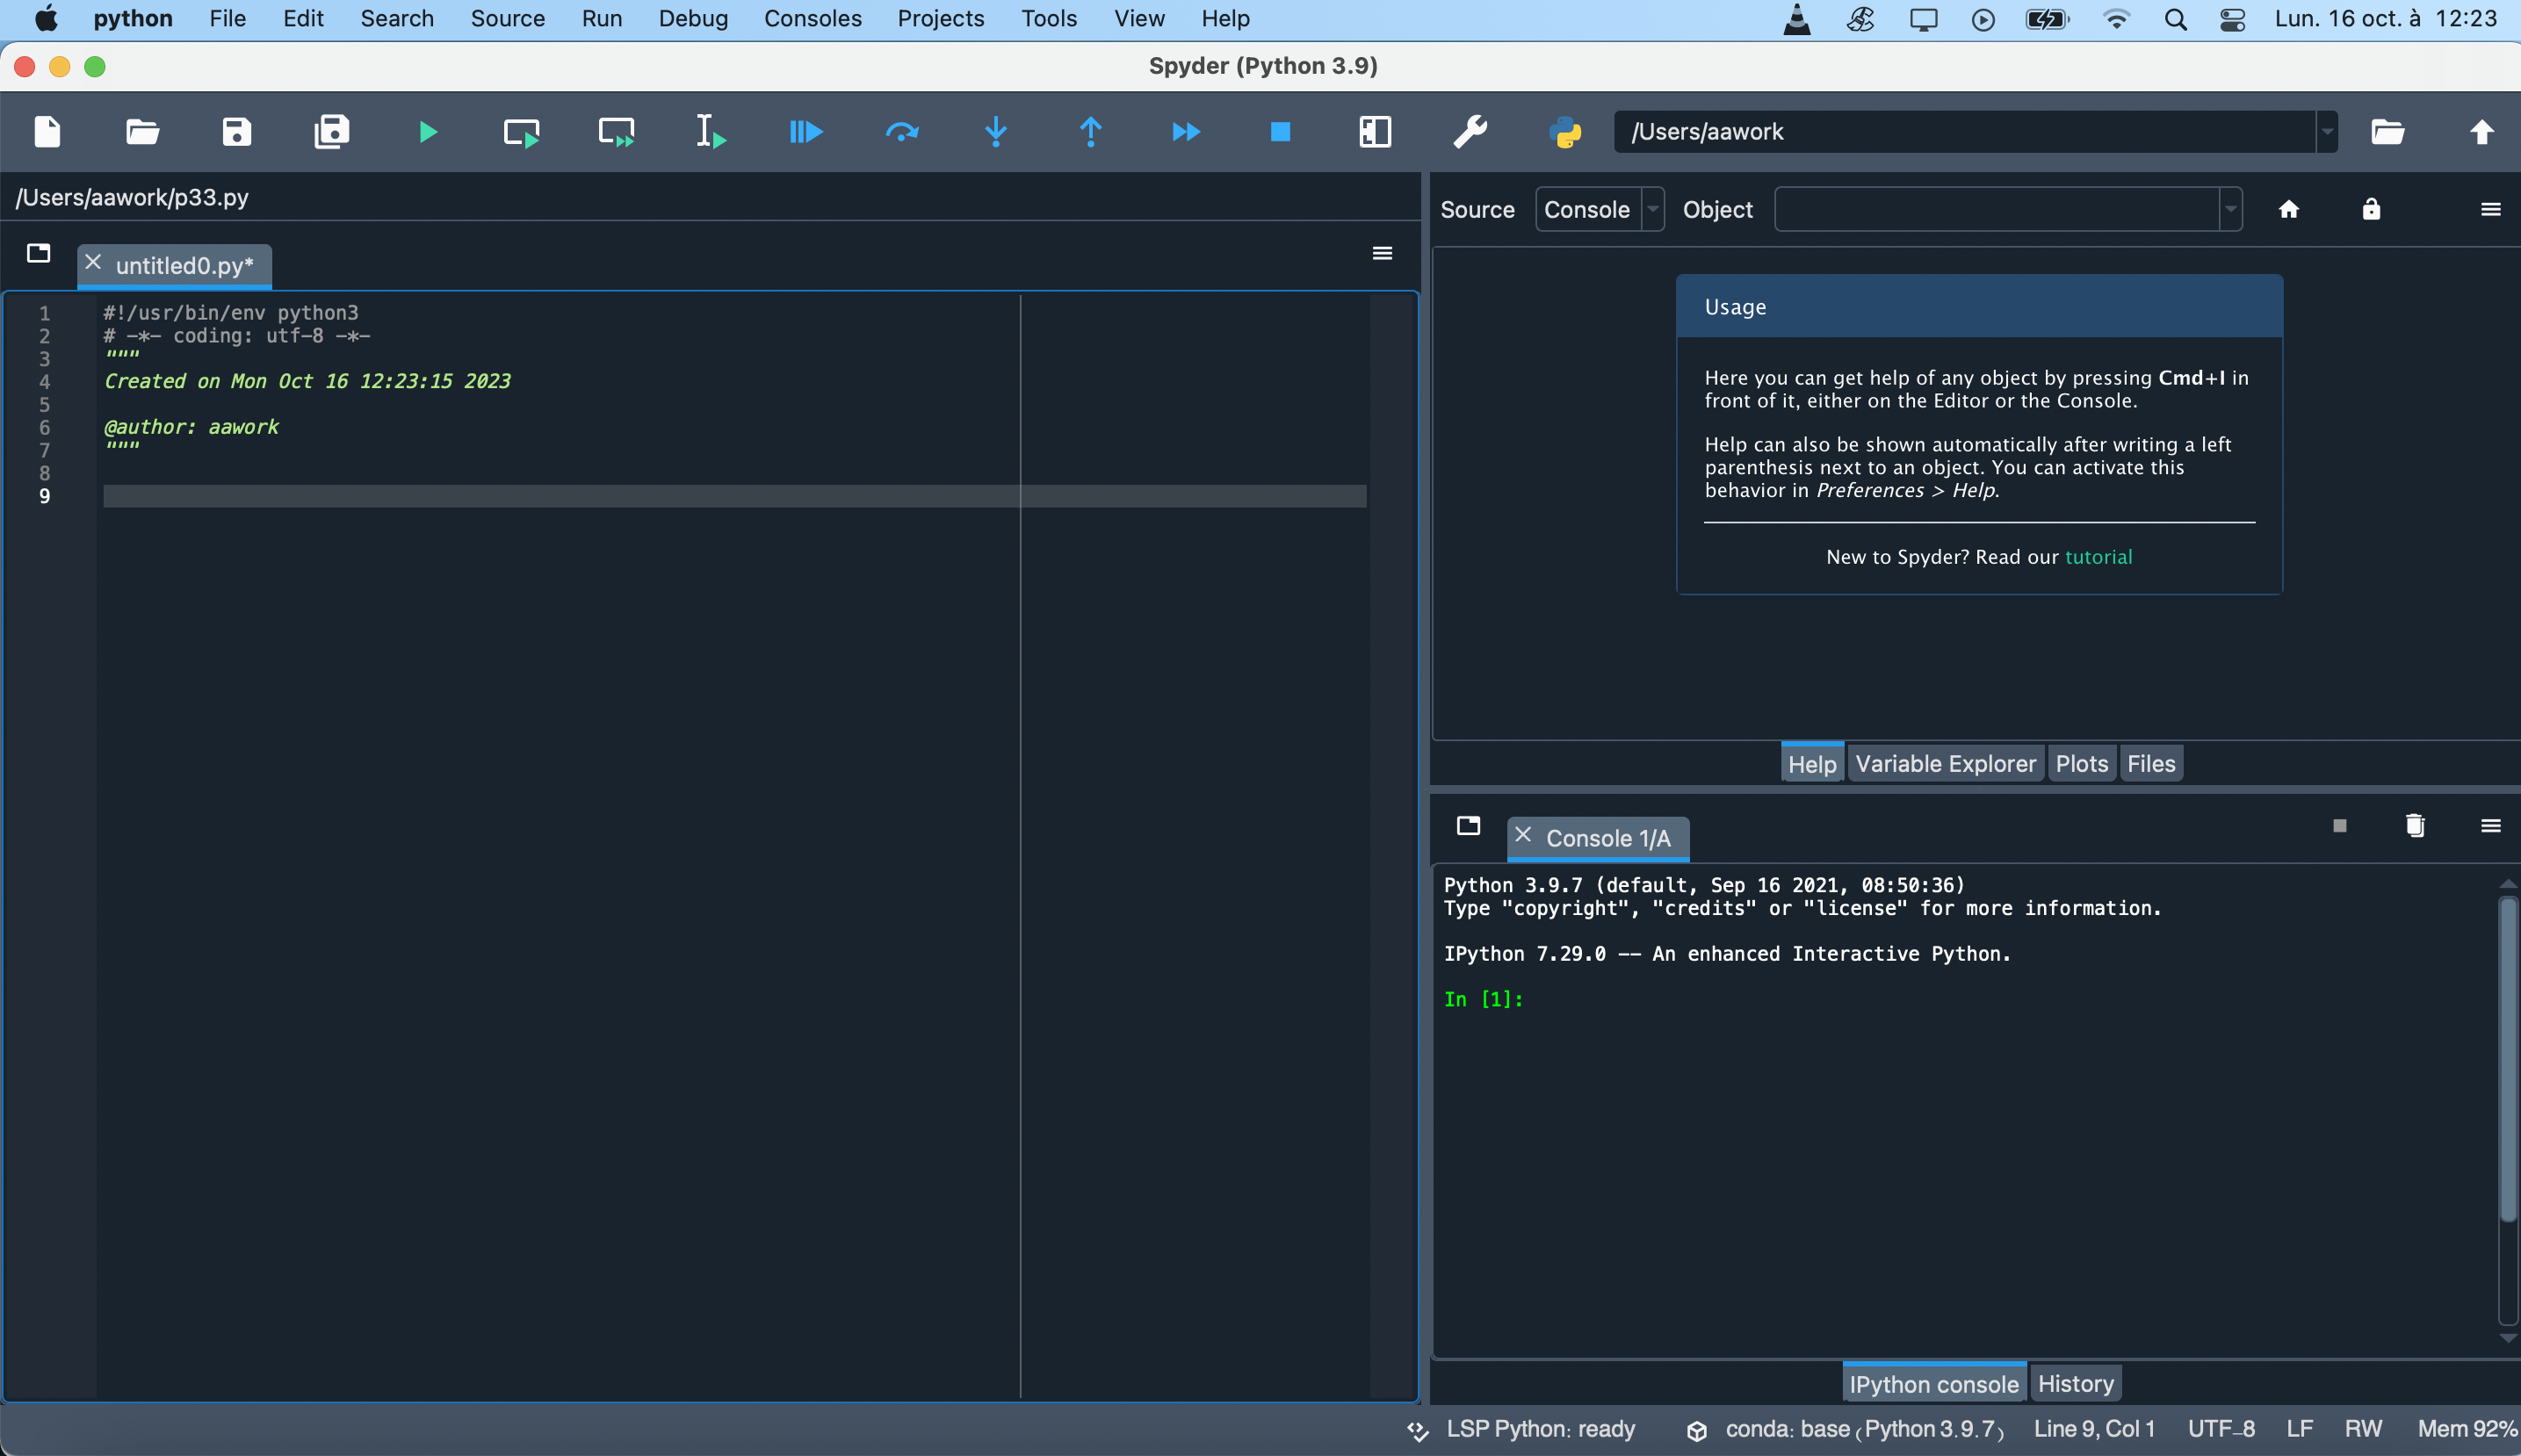
\includegraphics[height=7cm]{./png/menu-spyder}
\end{center}
\end{figure}

\end{enumerate}
\clearpage

%--organisation script python
\subsection{Organisation d'un script Python}
Un script python est structur\'e en trois parties
\begin{enumerate}
\item Ent\^ete de fichier script pour caract\`eres sp\'eciaux/accentu\'es
\begin{enumerate}
\item Pour les caract\`eres accentués correspondant aux principales langues d'Europe de l'ouest
\begin{lstlisting}[language={Python}]
# -*- coding:Latin-1 -*-
\end{lstlisting}

\item Pour la prise en compte du syst\`eme de codage mondial sur deux octets appel\'e Unicode
\begin{lstlisting}[language={Python}]
# -*- coding:Utf-8 -*-
\end{lstlisting}
\end{enumerate}
\item liste des modules \`a importer
\item liste des fonctions d\'efinies par l'utilisation
\item mise en donn\'ees du probl\`eme et ex\'ecution des fonctions
\end{enumerate}

L'exemple suivant relatif \`a la r\'esolution de l'\'equation du premier degr\'e montre une telle architecture.

\lstinputlisting[language=Python]{./codes/equa.py}


L'ex\'ecution du script en ligne de commande donne les r\'esultats suivants :
\begin{lstlisting}[language={Python}]
python equa.py 
Pas de solution
Infinite de solutions
a= 1
b= -5
x= 5.0
\end{lstlisting}

%--equation
\clearpage
\begin{enumerate}
\item Dans l'environnement Spyder, on charge le fichier equa.py. Le script appara\^it donc dans le bandeau de gauche.
\begin{figure}[h]
\begin{center}
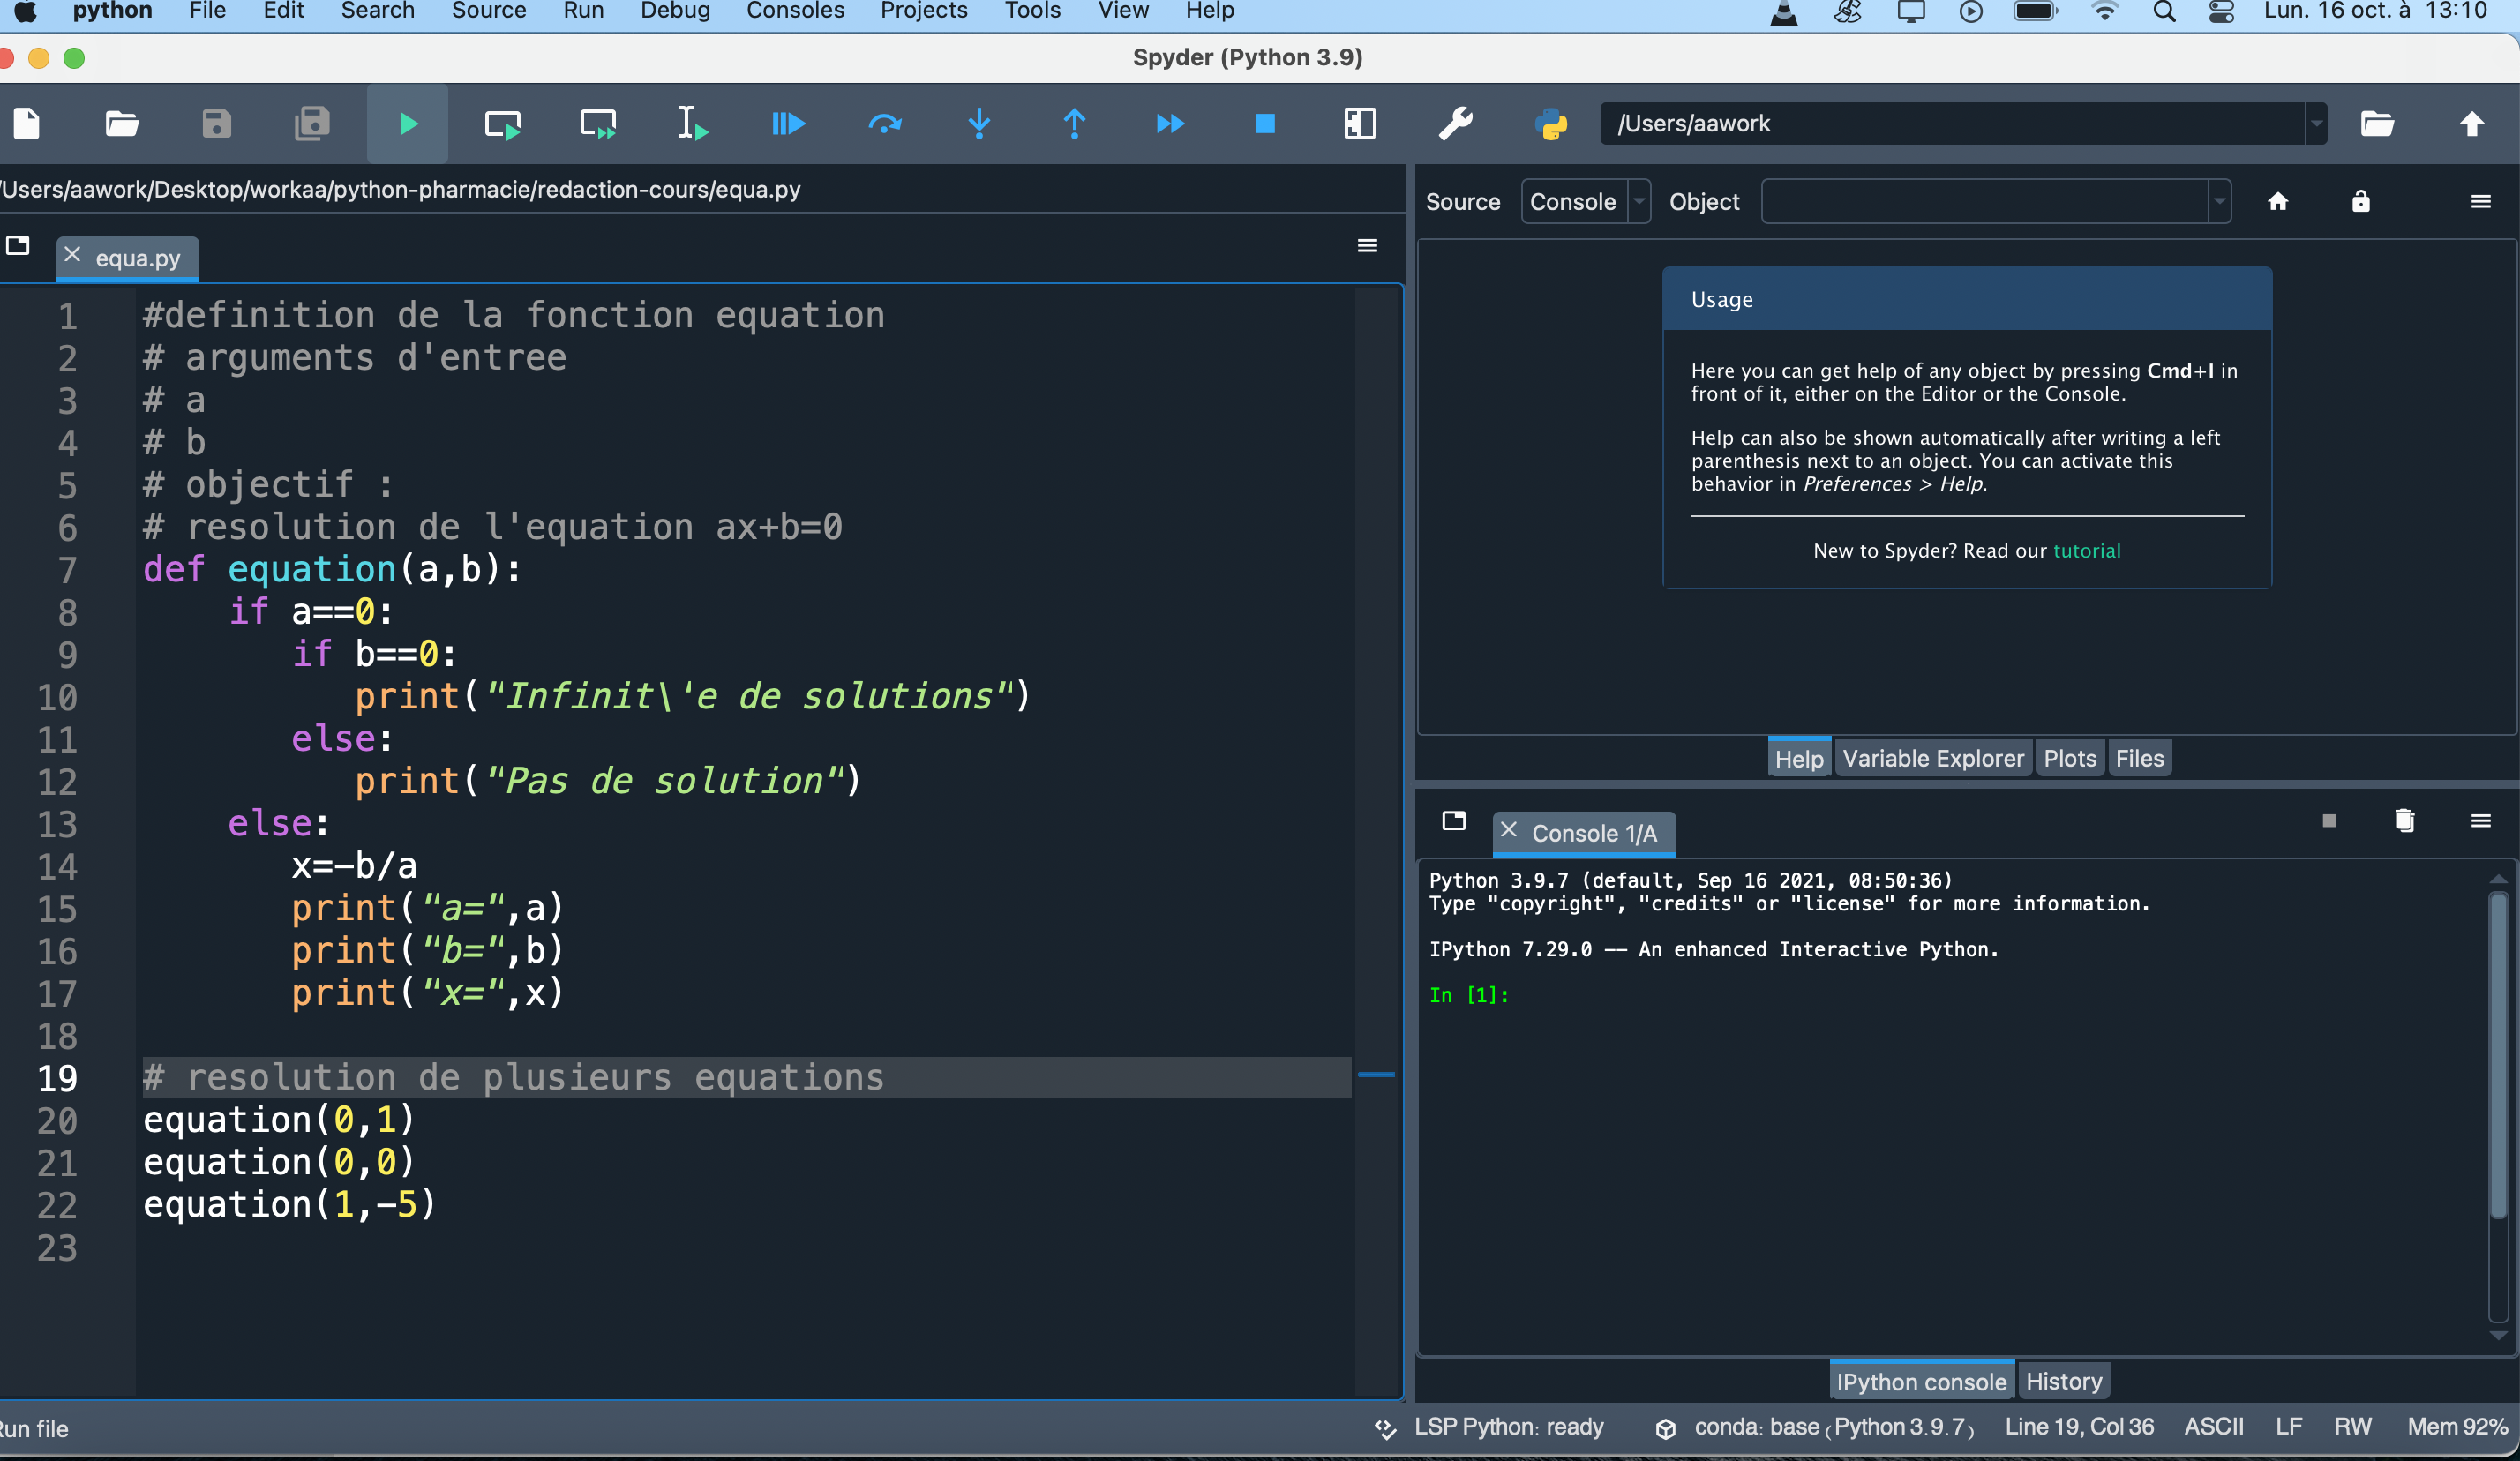
\includegraphics[height=8cm]{./png/equation.png}
\end{center}
\end{figure}
\item puis on appuie sur la touche F5 pour lancer l'ex\'ecution de celui-ci. Le r\'esultat est alors visible dans la console. En cliquant sur l'ic\^one \textbf{Variable Explorer}, il est possible de regarder le contenu es variables globales qui auront \'et\'e cr\'e\'es par le script. Dans le cas pr\'esent, il n'y a pas de telles variables. En effet, seule la variable $x$, locale \`a la fonction equation a \'et\'e cr\'ee. Elle n'est pas accessible hors de cette fonction. Il est donc n\'ecessaire de l'afficher pour en avoir connaissance.  Ce qui est r\'ealis\'e dans le script.
\begin{figure}[h]
\begin{center}
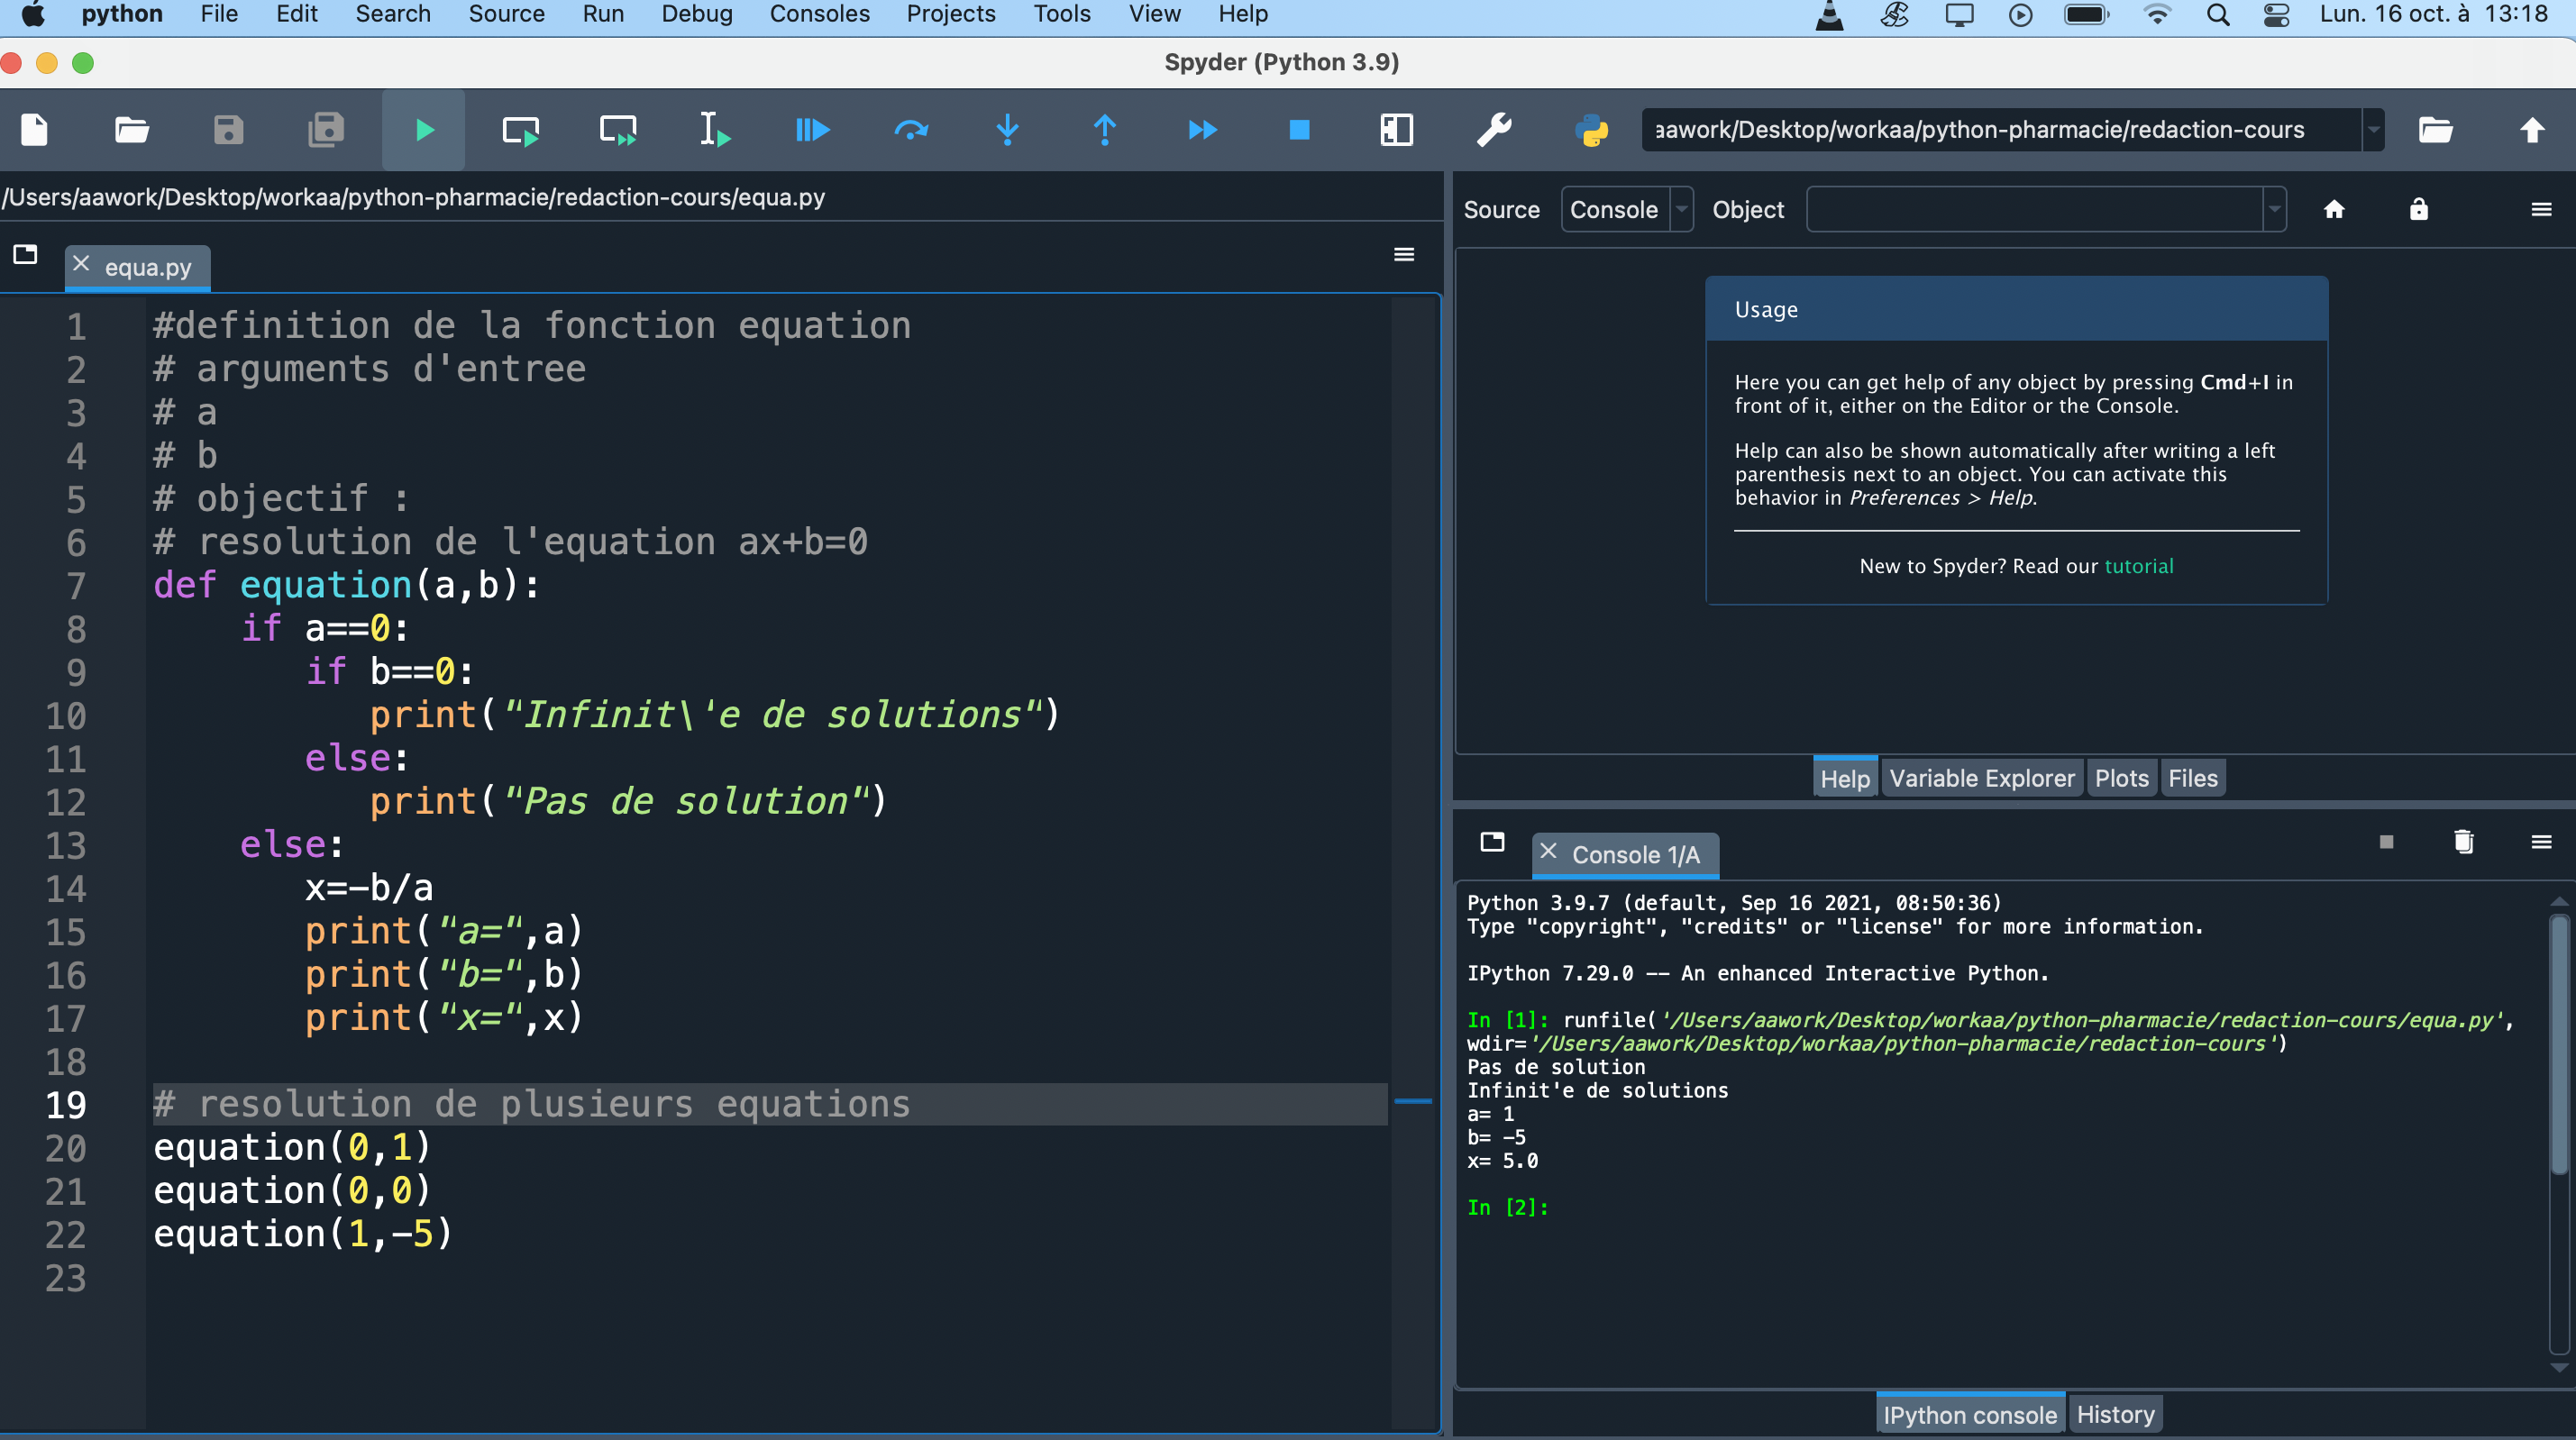
\includegraphics[height=8cm]{./png/equation-resultat.png}
\end{center}
\end{figure}
\end{enumerate}

\clearpage
%--manipulation de fichiers
\subsection{Manipulation fichiers en lecture/\'ecriture}

\subsubsection{D\'efinition}
\begin{leftbar}
Les fichiers peuvent \^etre manipul\'es en
\begin{enumerate}
\item \'ecriture
\item lecture
\item ajout en fin de fichier
\end{enumerate}
Bien noter la pr\'esence du nom logique diff\'erent du nom physique correspondant au fichier pr\'esent dans le r\'epertoire de travail.  La fonction open ne manipule que des chaines de caract\`eres. Il faut donc convertir les nombres r\'eels ou entiers \`a l'aide de l'instruction \textbf{str}.
\end{leftbar}
\subsubsection{Exemple}

\lstinputlisting[language=Python]{./codes/fichier.py}

Le fichier 'toto.txt' contient les lignes suivantes 
\verbatiminput{toto.txt}

Dans l'environnement Spyder, on obtient
\begin{figure}[h]
\begin{center}
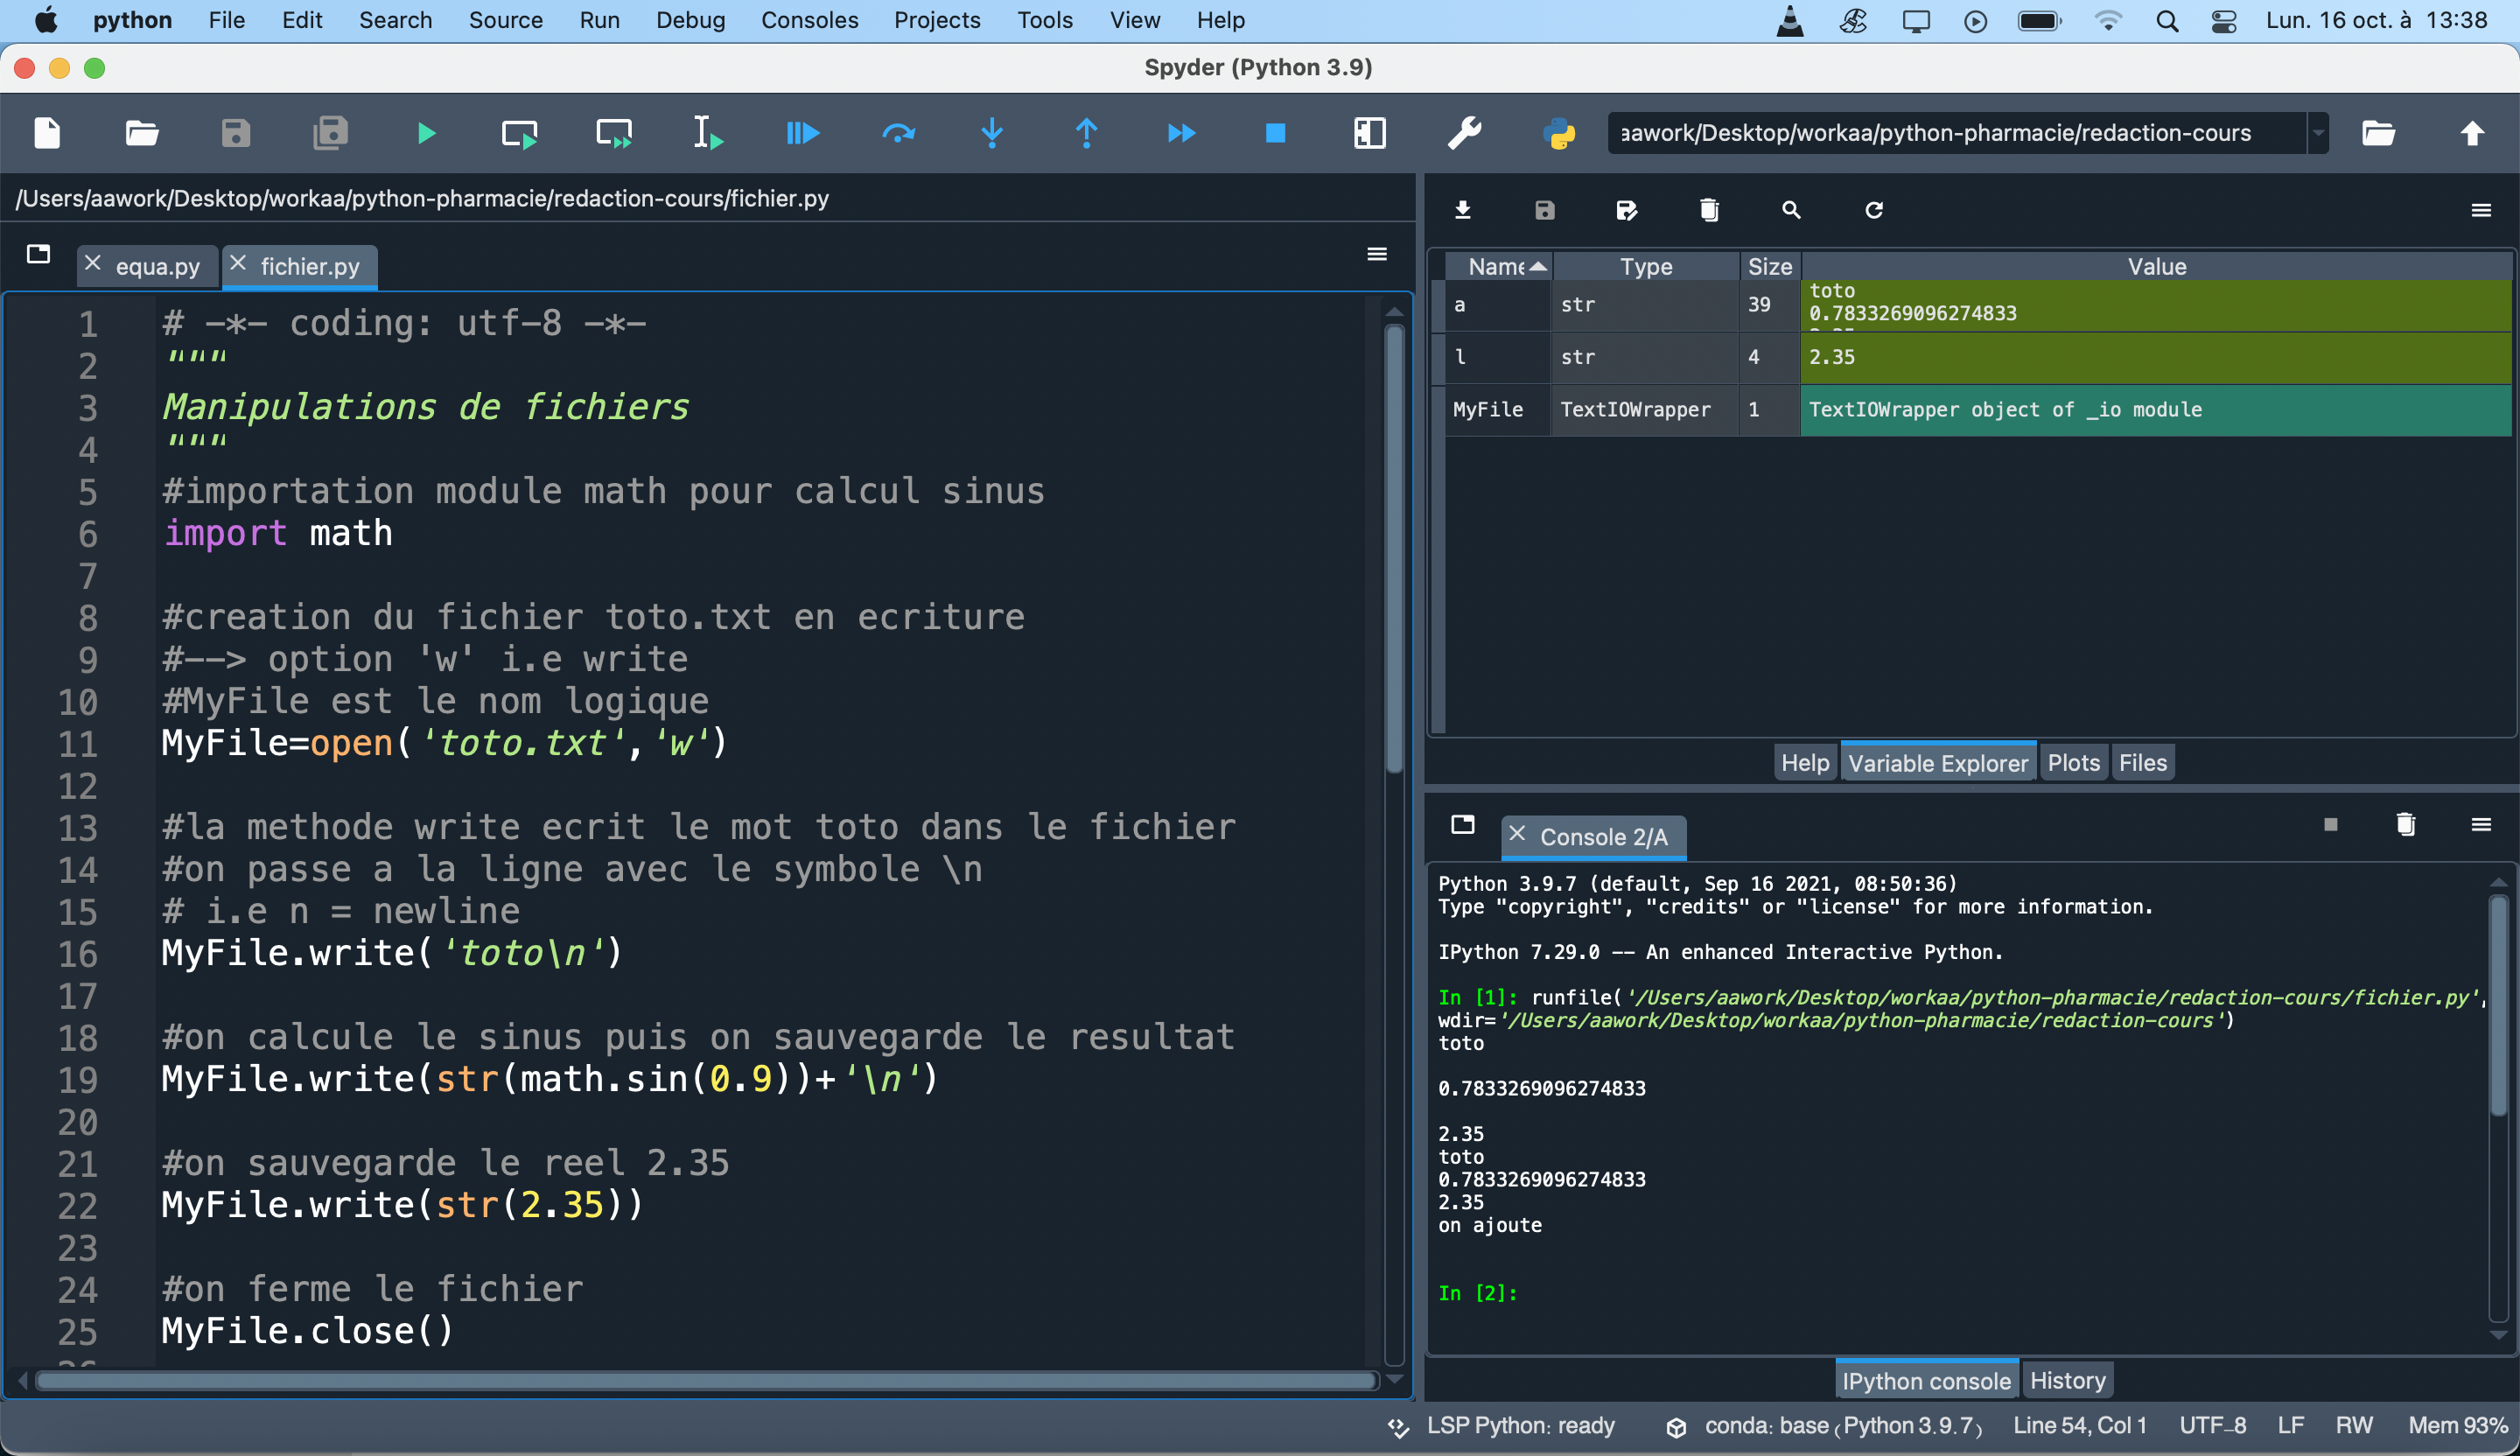
\includegraphics[height=8cm]{./png/fichier-spyder.png}
\end{center}
\end{figure}

En cliquant sur la variable \textbf{a}, on obtient la cha\^ine de caract\`eres. Celle-ci est de type \textbf{str} et occupe \textbf{39} octets.
\begin{figure}[h]
\begin{center}
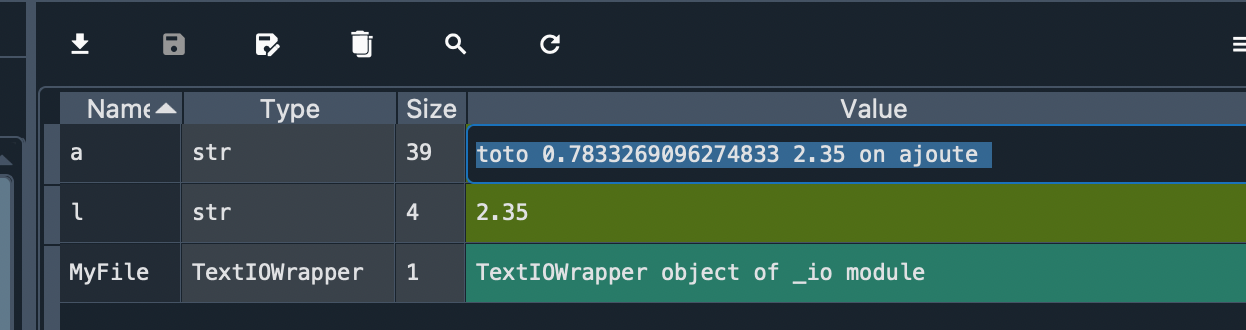
\includegraphics[height=3cm]{./png/fichier-chaine.png}
\end{center}
\end{figure}
%--methodes fichiers
\clearpage
\begin{itemize}
\item On remarque que l'objet MyFile permettant d'acc\'eder au fichier 'toto.txt' ne peut pas \^etre visualis\'e dans Spyder. Enfin en tapant MyFile. , il appara\^it un menu d\'eroulant permettant d'acc\'eder \`a toutes les m\'ethodes i.e. fonctions possibles. 
\begin{figure}[h]
\begin{center}
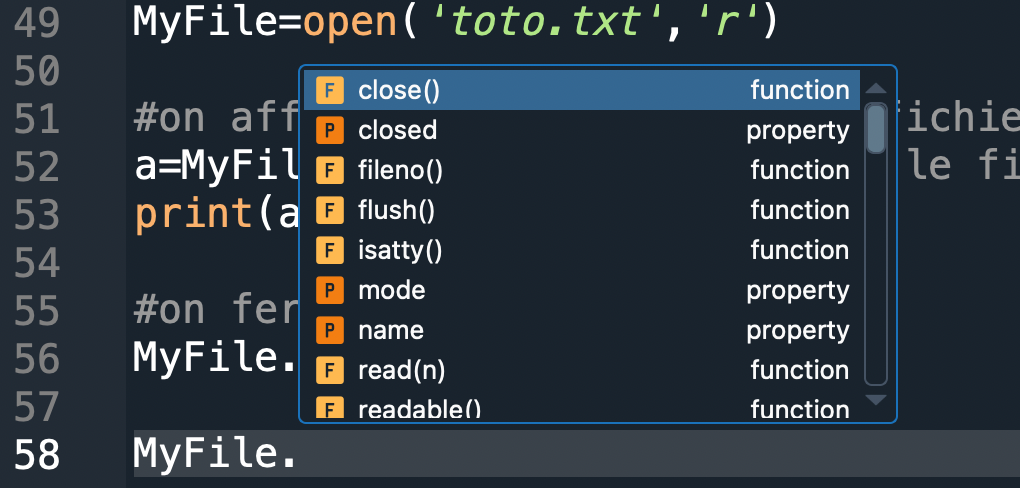
\includegraphics[height=3cm]{./png/fichier-methodes-a.png}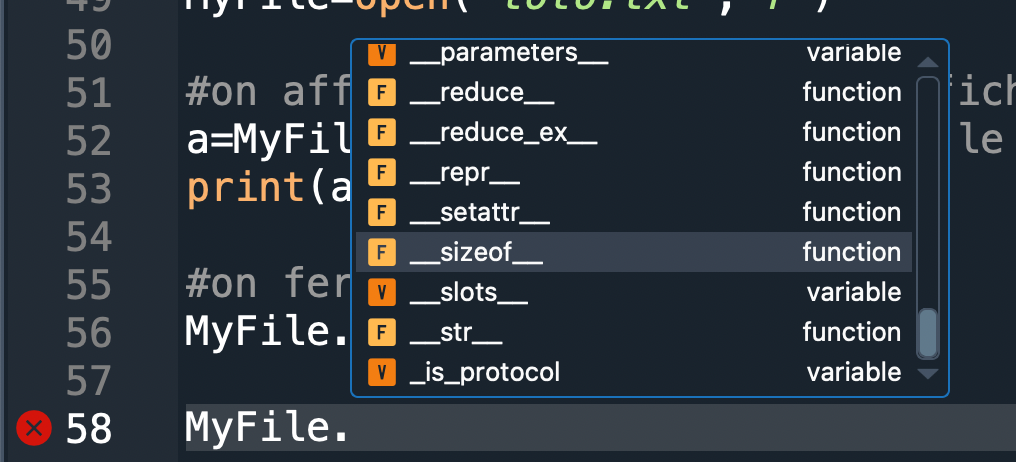
\includegraphics[height=3cm]{./png/fichier-methodes-b.png}
\end{center}
\end{figure}
\item En s\'electionnant par exemple write(), une aide est visible et la fonction est \'ecrite dans le code python. 
\begin{figure}[h]
\begin{center}
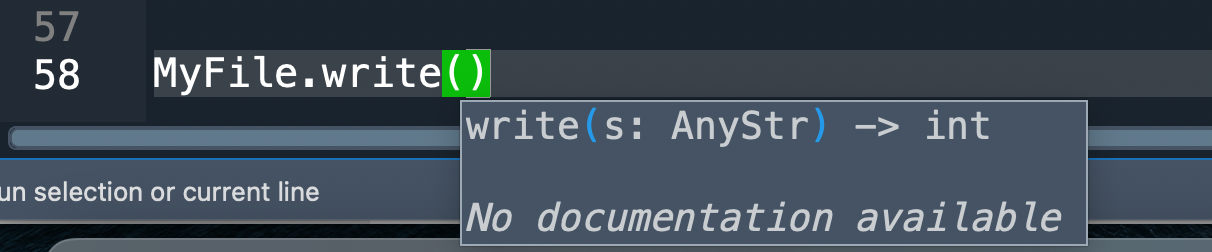
\includegraphics[height=2cm]{./png/fichier-write.png}
\end{center}
\end{figure}
\end{itemize}

%--clearpage
\subsubsection{Exercice}
\begin{leftbar}
On demande d'\'ecrire un script python \'ecrivant dans un fichier nomm\'e 'fontaine.txt', les premiers vers de la onzi\`eme fable de la Fontaine, 
\verbatiminput{fable.txt}
On \'ecrira ensuite le nombre 1668 \`a la cinqui\`eme ligne.
On relira ensuite ligne par ligne le fichier cr\'e\'e puis on affichera chacune de ces lignes
\end{leftbar}
\subsubsection{Correction}
\lstinputlisting[language=Python]{./codes/fable.py}

\clearpage
%--types de donnees
\section{Types de donn\'ees}
Nous allons regarder les quatre types suivants
\begin{enumerate}
\item entier/r\'eels
\item vecteur/matrice
\item chaines de caractères
\item listes
\end{enumerate}

\subsection{entiers/réels}

\subsubsection{Définition}
Pour créer une variable de type entier ou réel, il suffit d'utiliser une simple égalité \textbf{variable=nombre}.
Contrairement aux langages typés tels que le fortran , Pascal, C etc..., il n' y a pas de déclaration de type

\subsubsection{Exemple}
\lstinputlisting[language=Python]{./codes/entier-reel.py}

Dans l'environnement spyder, en cliquant sur l'onglet Variable Explorer, on observe bien le type des données manipulées dans le script.

\begin{figure}[h]
\begin{center}
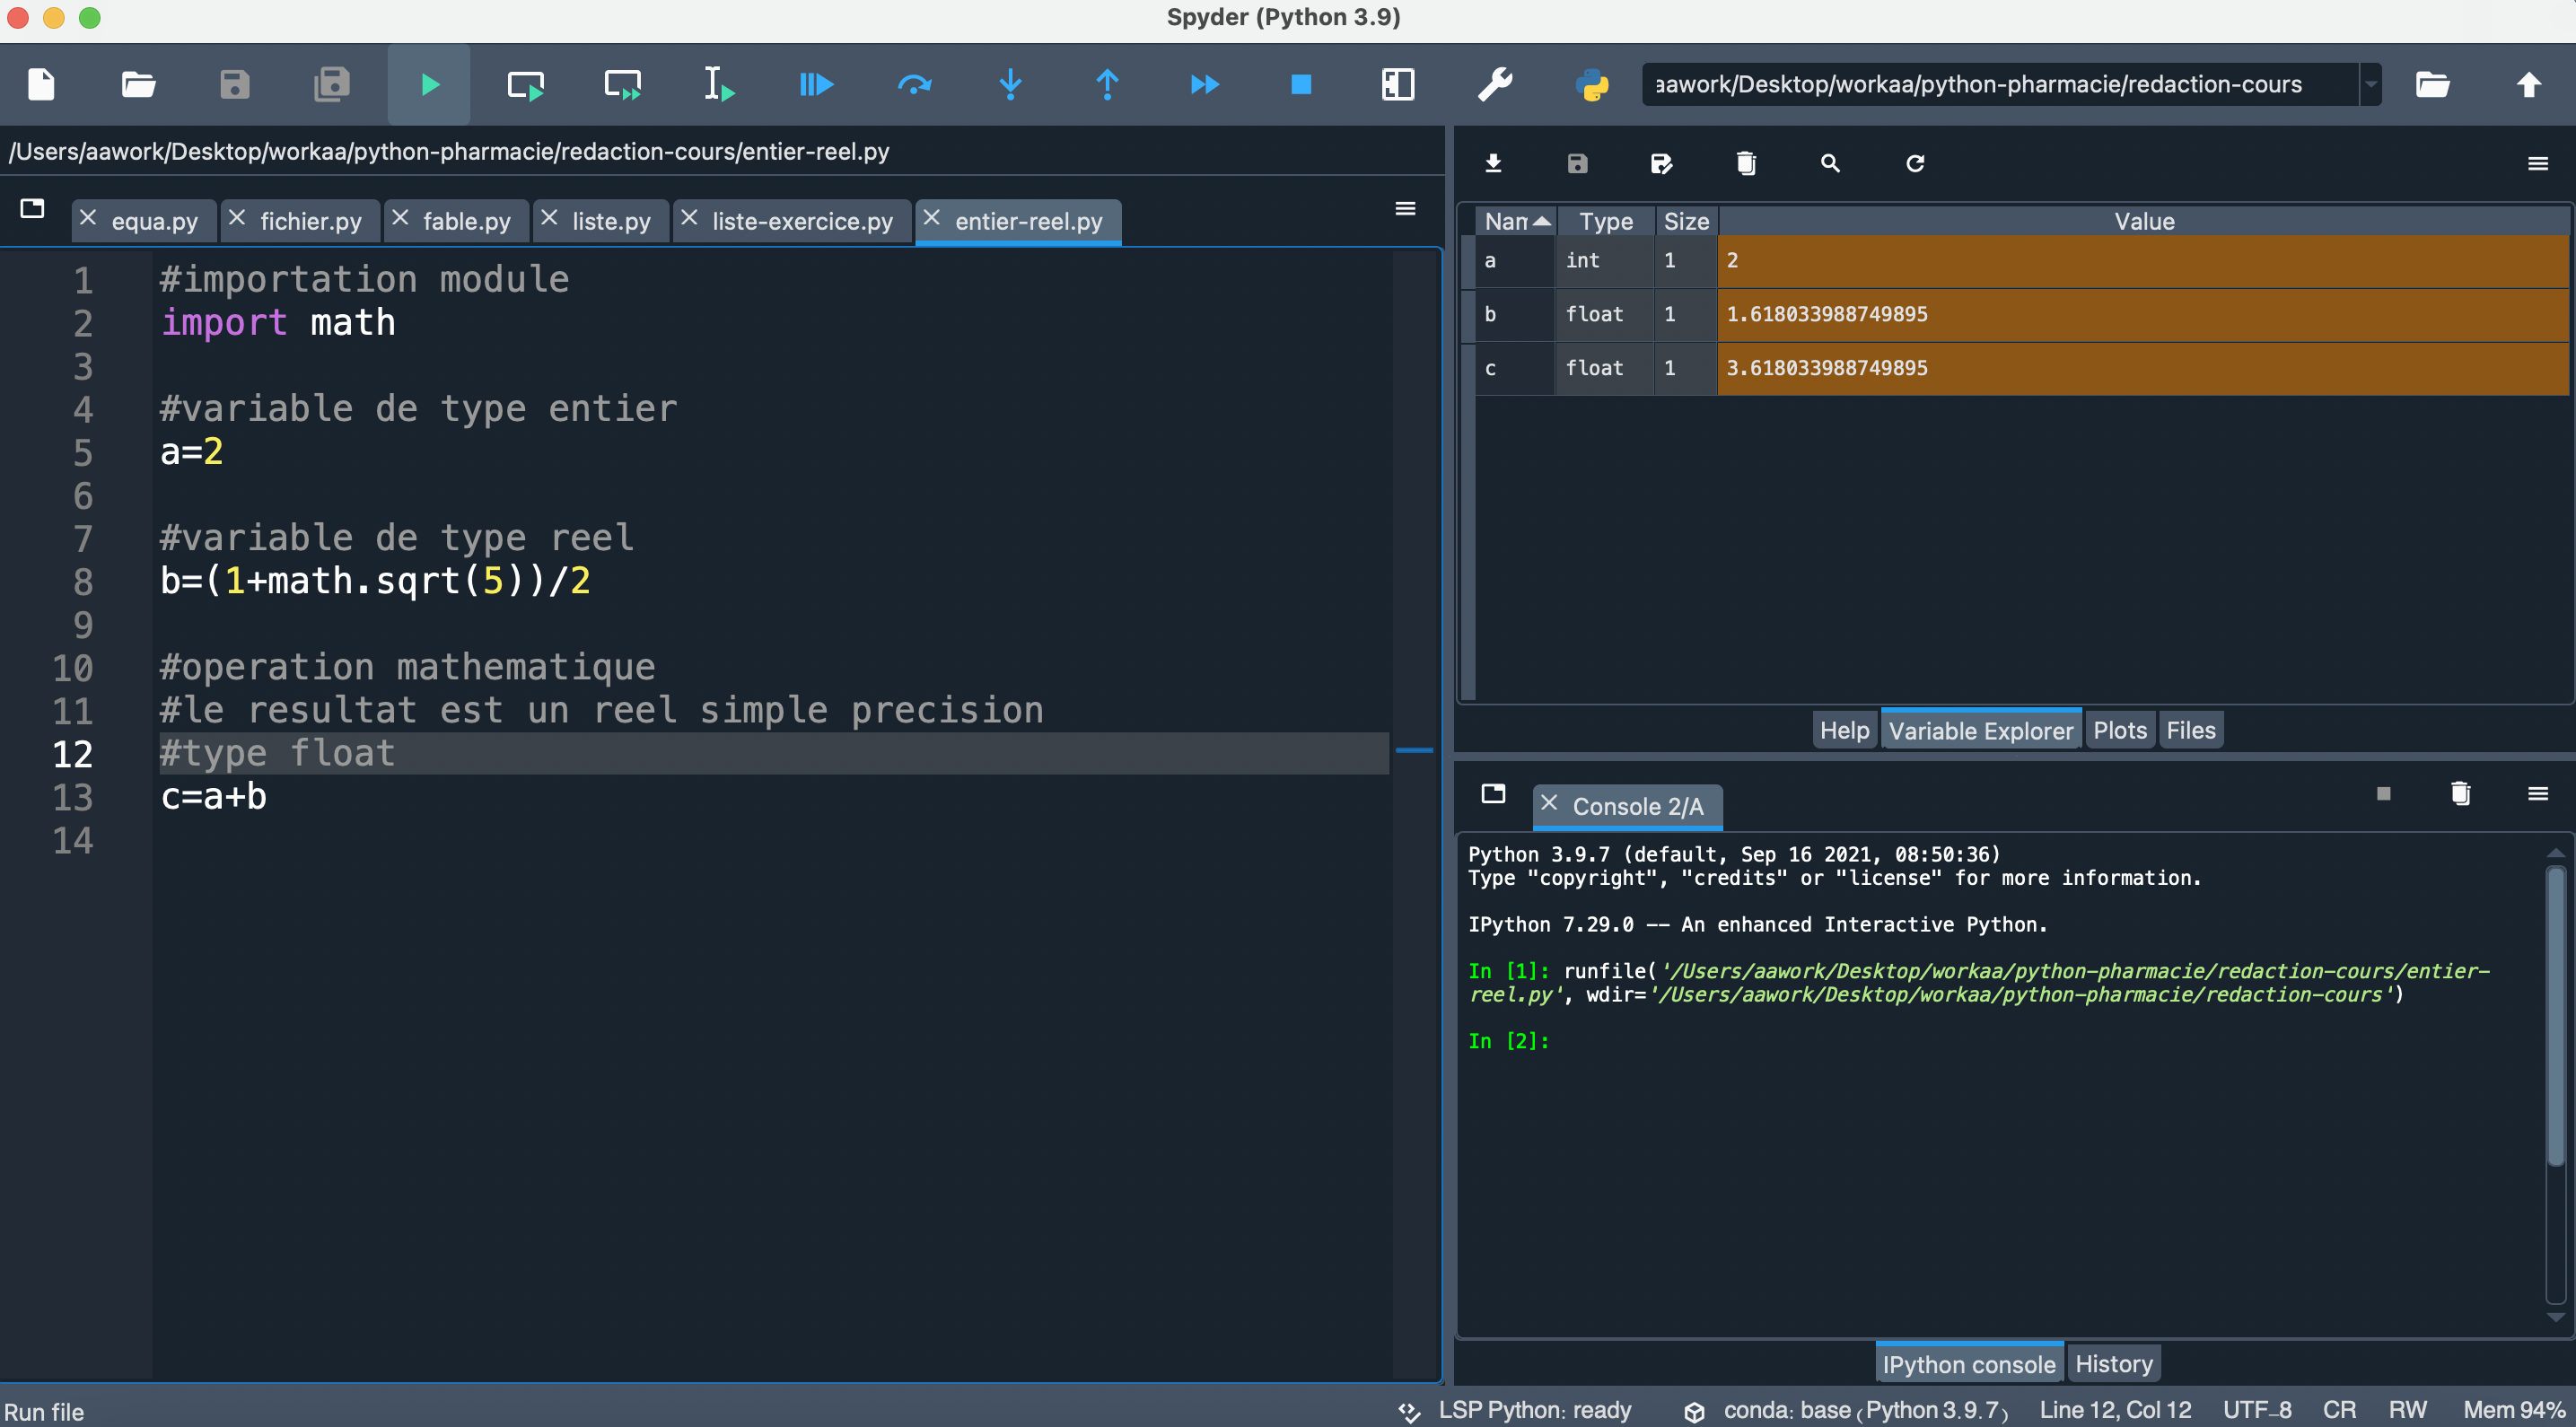
\includegraphics[height=7cm]{./png/entier-reel.png}
\end{center}
\end{figure}

%--vecteurs/matrices
\clearpage
\subsection{vecteur/matrice}
\subsubsection{Définition}
La bibliothèque numpy permet de créer et de manipuler des vecteurs et matrices.
\subsubsection{Exemple}
\lstinputlisting[language=Python]{./codes/vecteur-matrice.py}

\begin{enumerate}
\item La création du vecteur \textbf{a} dans Spyder permet d'accéder à de nombreuses méthodes
\begin{figure}[h]
\begin{center}
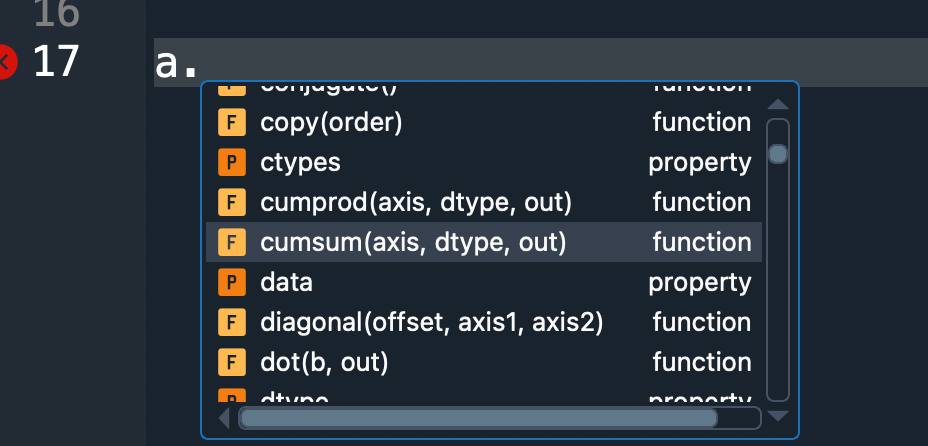
\includegraphics[height=2cm]{./png/methodes-vecteur.png}
\end{center}
\end{figure}
\item les fonctions de la sous bibliothèque \text{linalg}  commençant par n, sont accessibles en tapant .n comme indiqué ci-dessous.
\begin{figure}[h]
\begin{center}
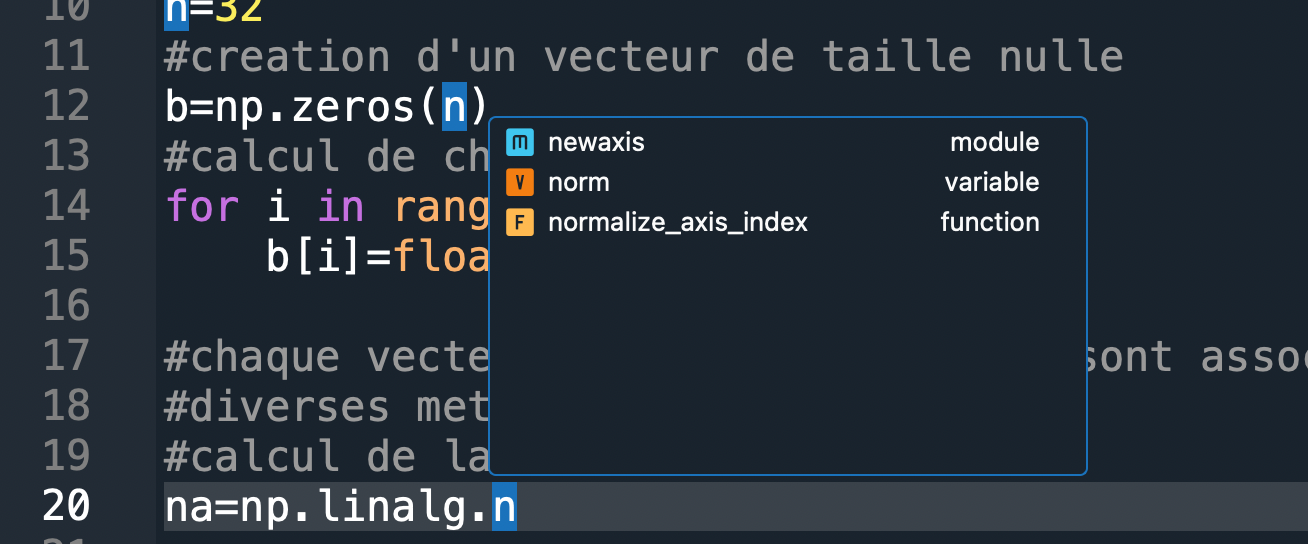
\includegraphics[height=2cm]{./png/np-linalg.png}
\end{center}
\end{figure}
\item Dans l'environnement sypder, il est possible d'accéder au type des variables définies ainsi qu'à leur contenu.
\begin{figure}[h]
\begin{center}
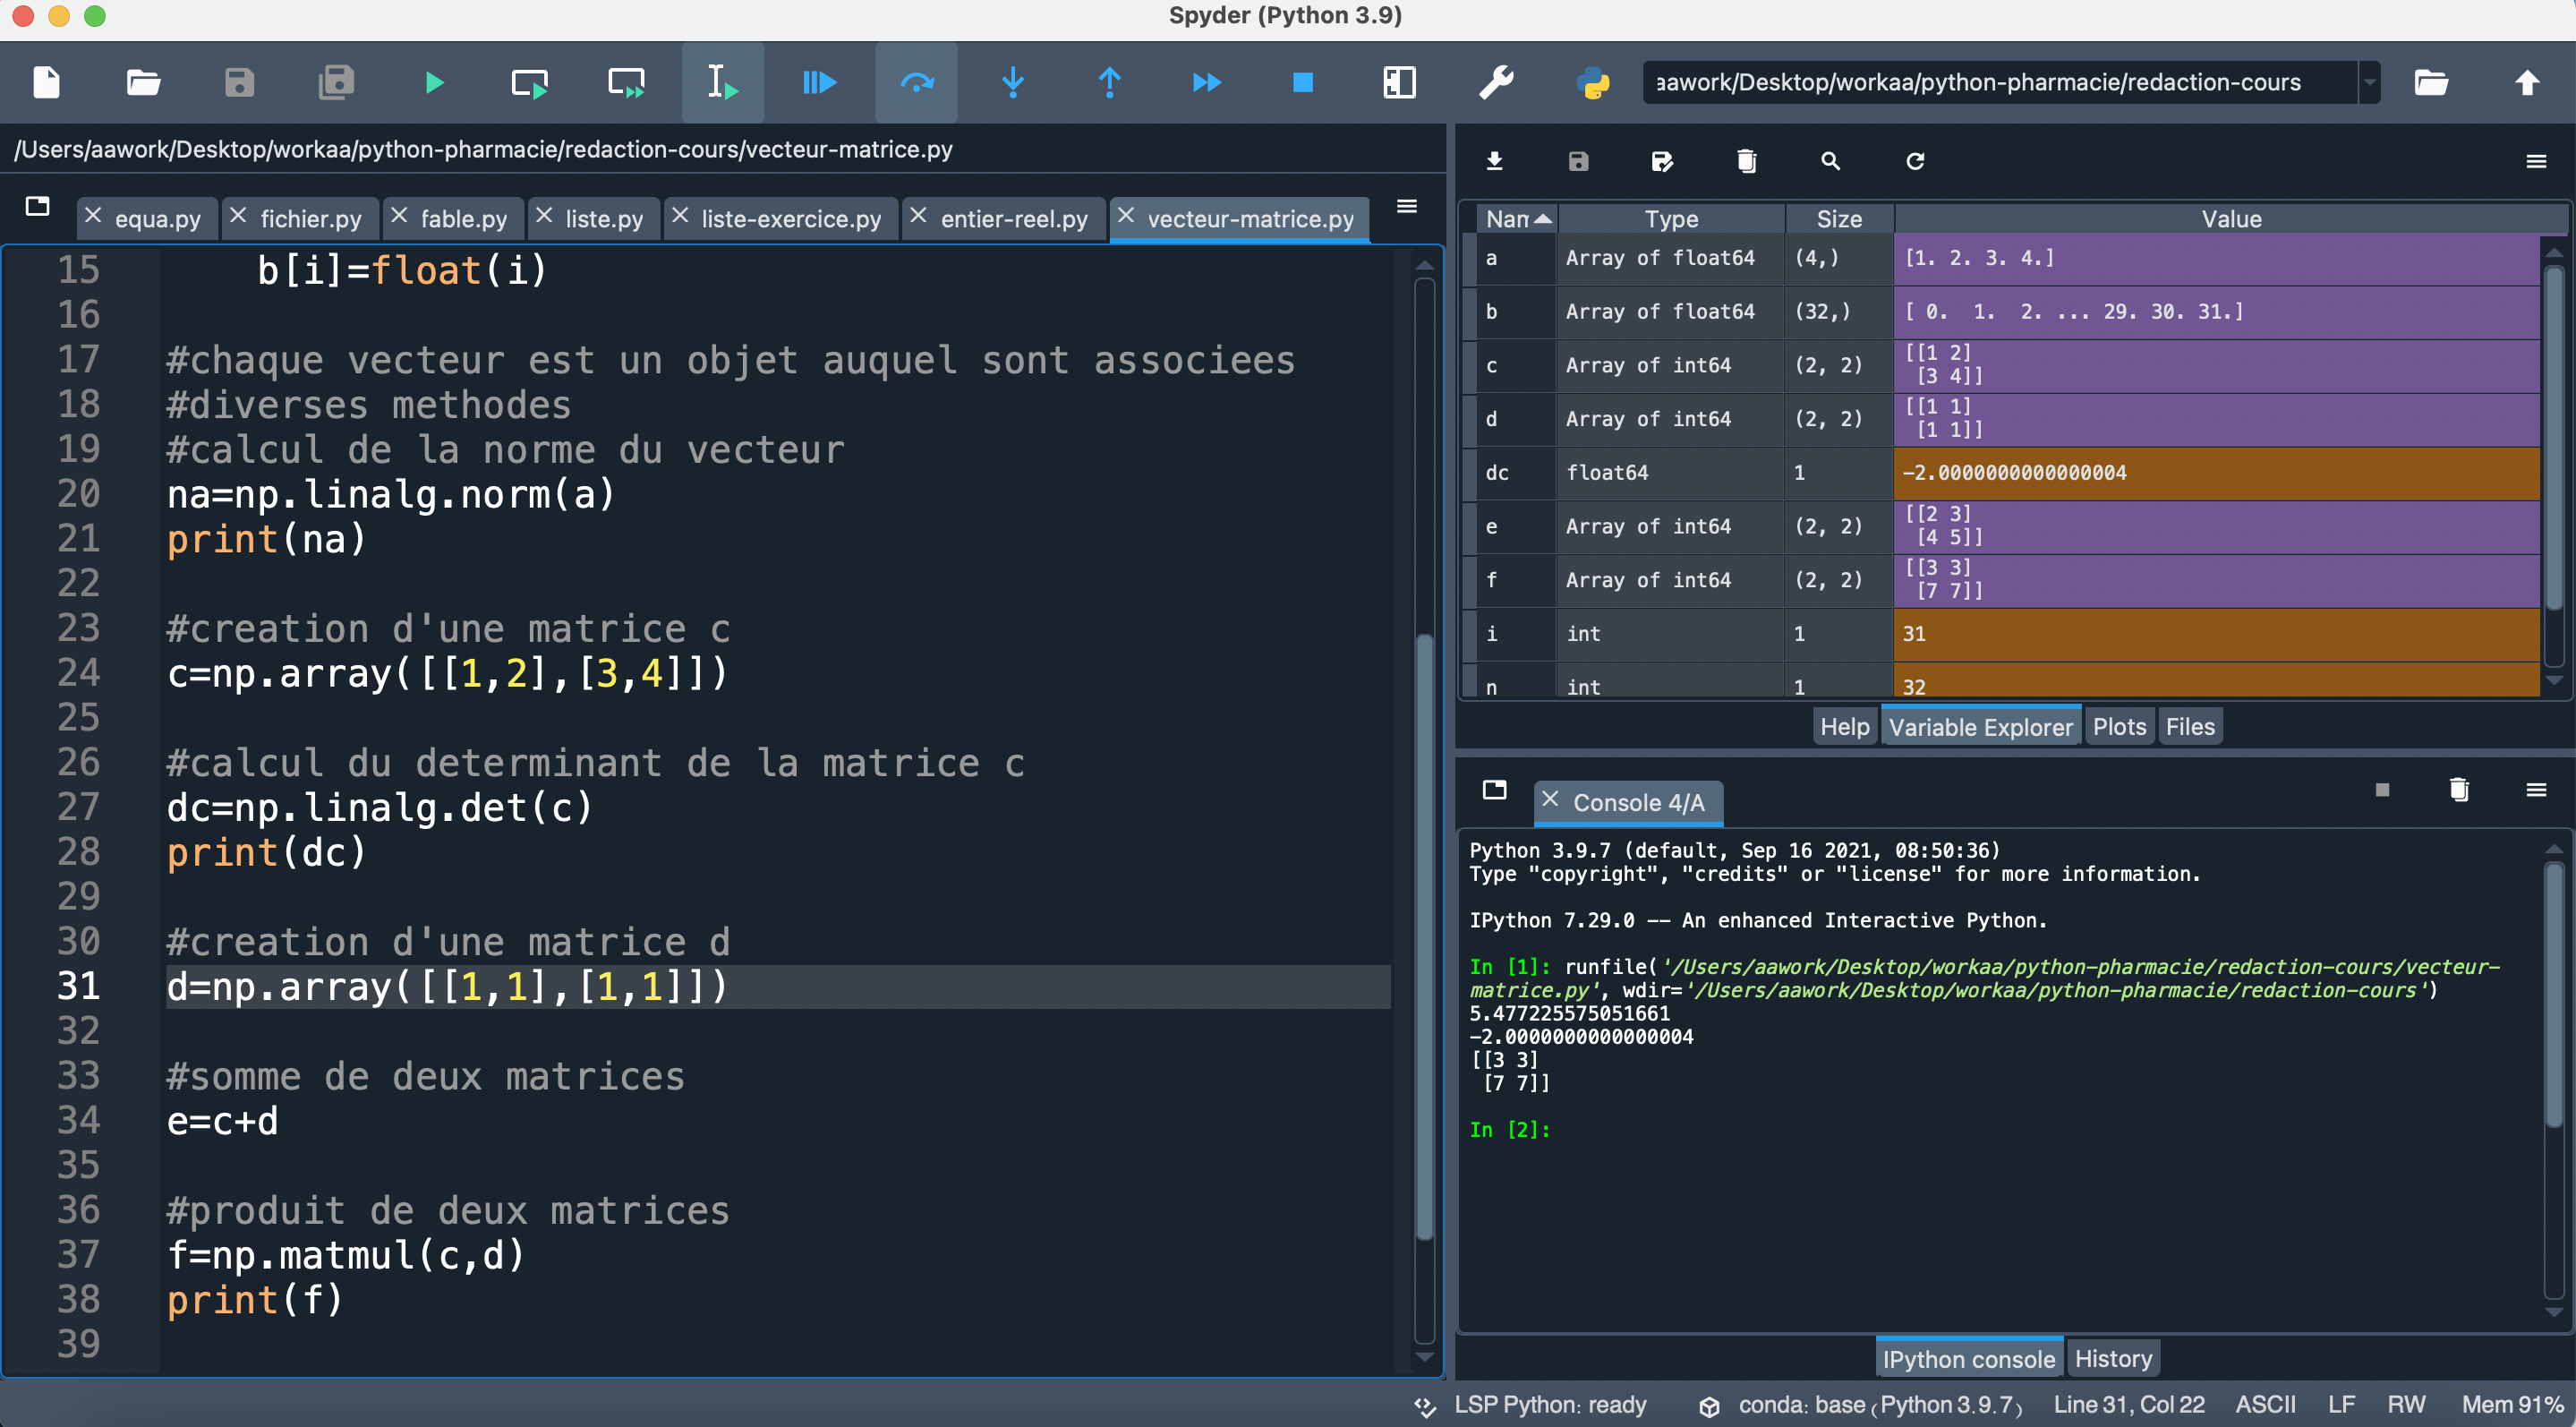
\includegraphics[height=10cm]{./png/vecteur-matrice.png}
\end{center}
\end{figure}
\end{enumerate}

%--chaines de caracteres
\clearpage
\subsection{Cha\^ines de caractères}
\subsubsection{Définition}
Les délimiteurs d'une cha\^ine de caractères peuvent être soit le symbole \textbf{'} soit \textbf{"}.
\subsubsection{Exemple}
Voici une présentation non exhaustive des manipulations possibles sur une liste 
\lstinputlisting[language=Python]{./codes/chaine.py}

Dans l'environnement sypder, il est possible d'accéder au type des variables alphanumériques définies ainsi qu'à leur contenu.
\begin{figure}[h]
\begin{center}
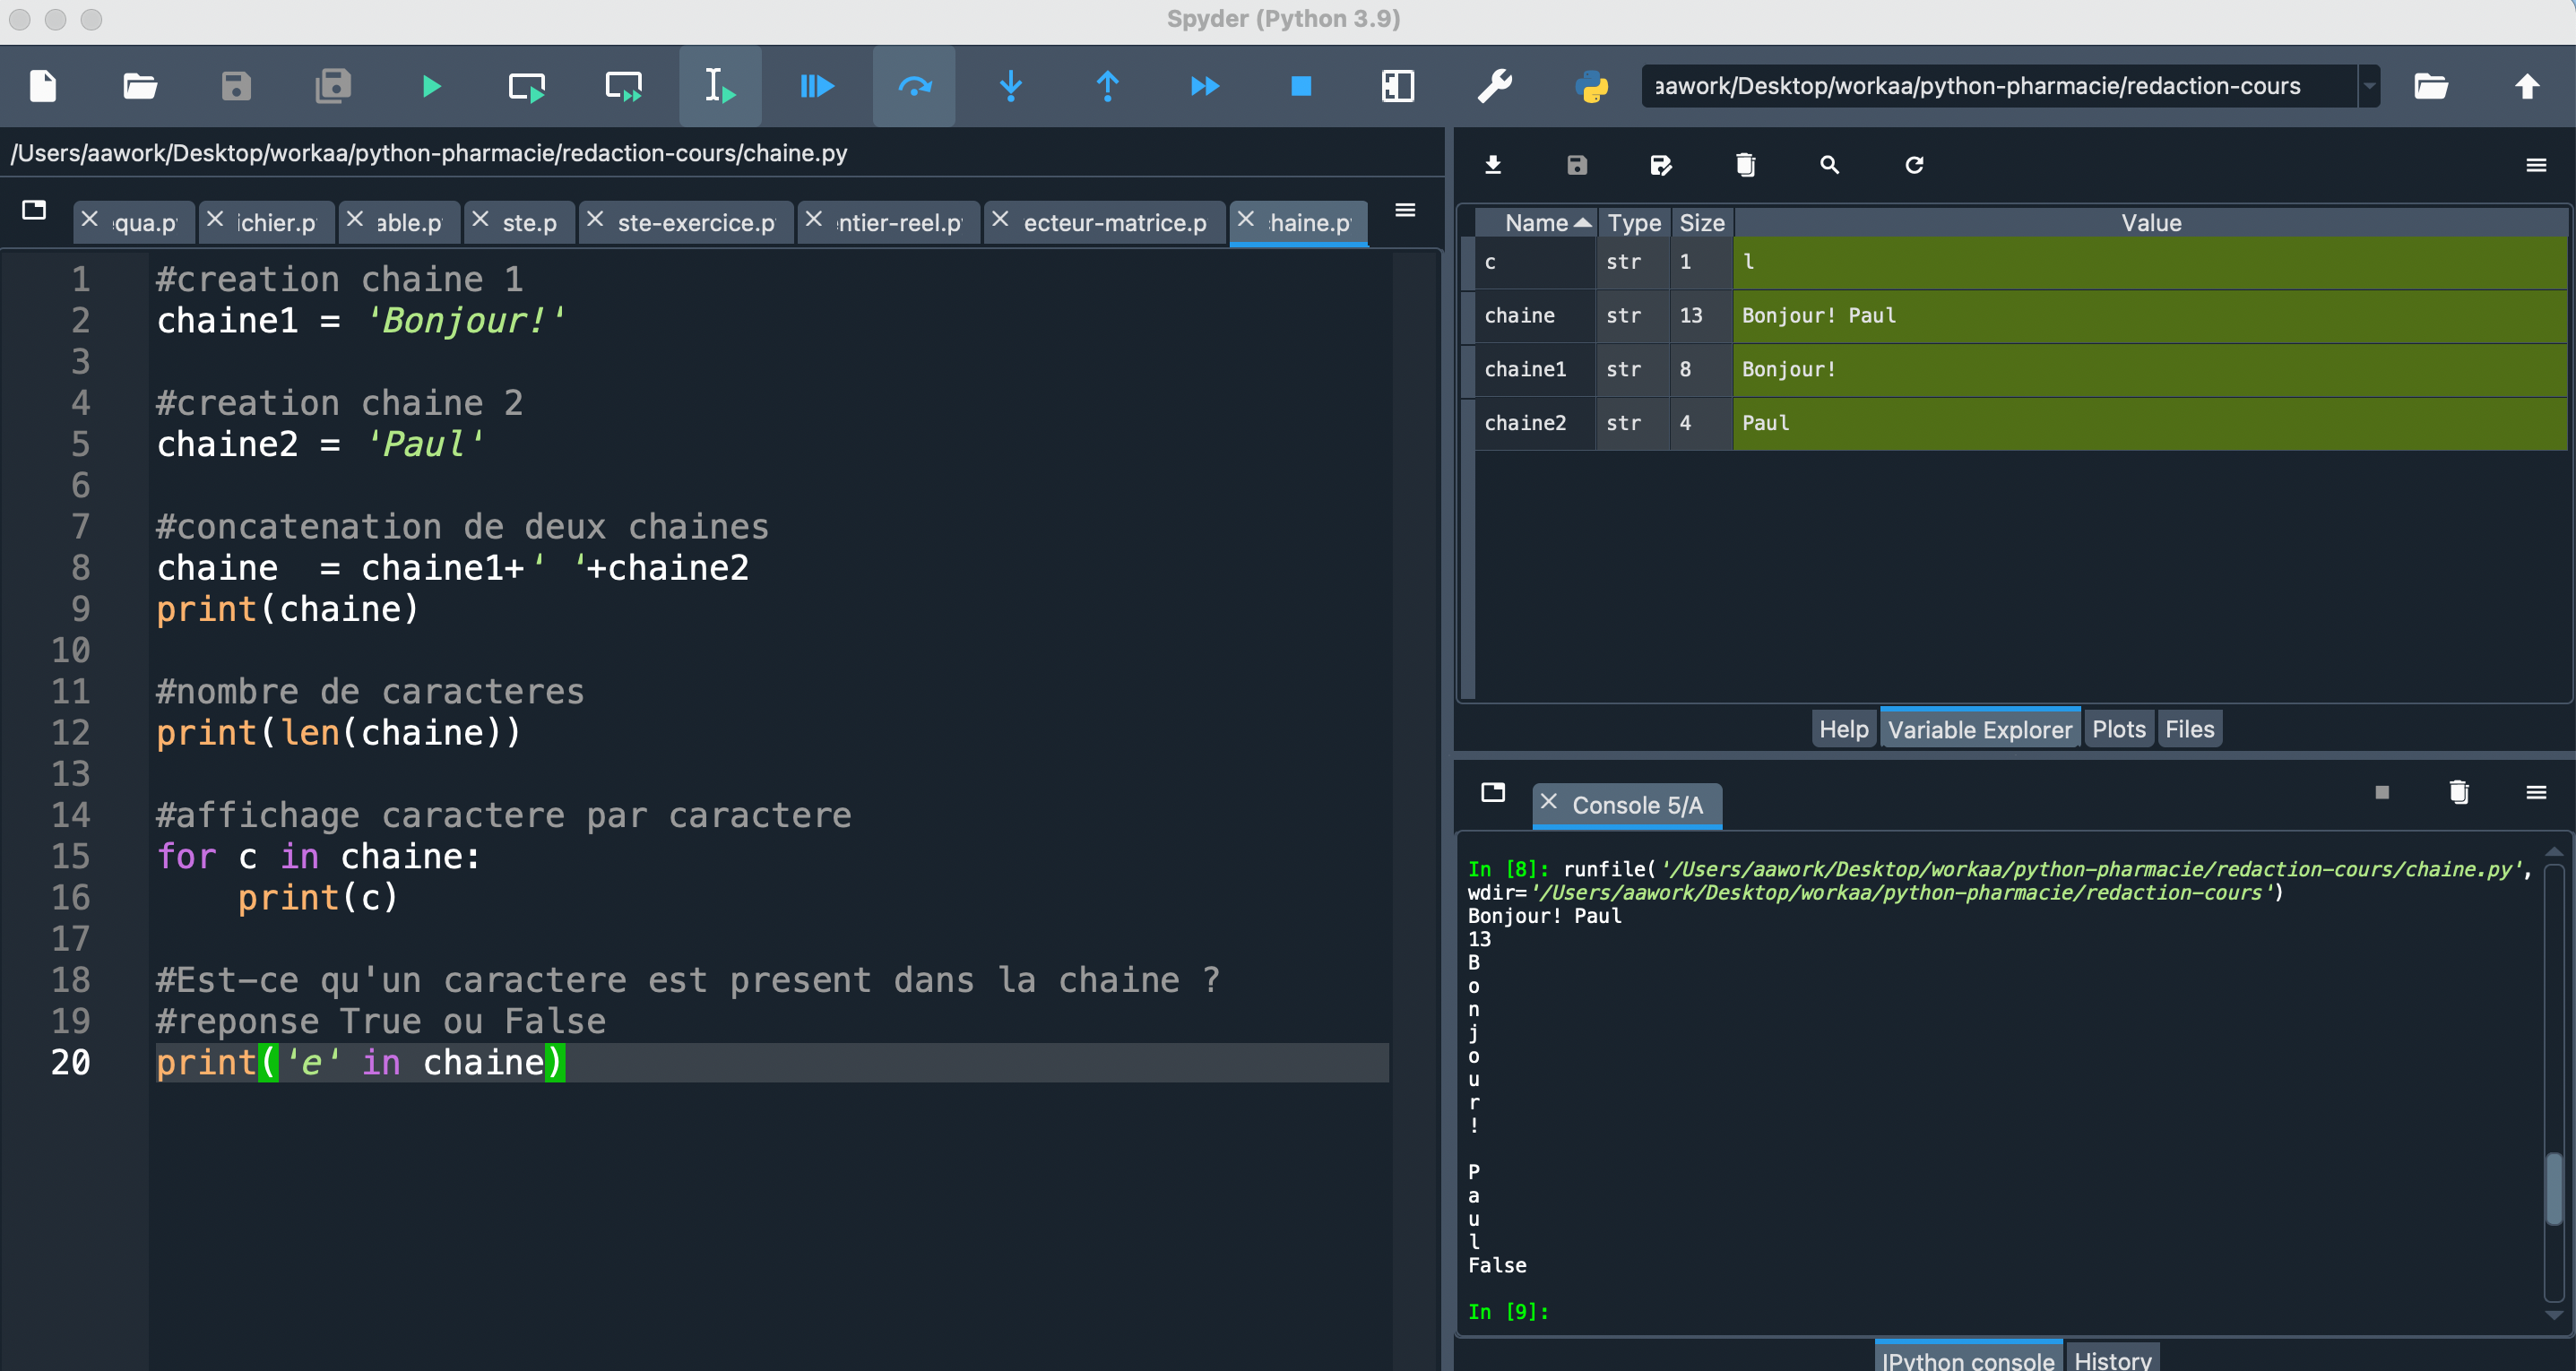
\includegraphics[height=10cm]{./png/chaine.png}
\end{center}
\end{figure}


%--listes
\clearpage
\subsection{Listes}
\subsubsection{Définition}
Une liste en python est une  variable dans laquelle on peut mettre plusieurs variables de type différents.
\subsubsection{Exemple}
Voici une présentation non exhaustive des manipulations possibles sur une liste 
\lstinputlisting[language=Python]{./codes/liste.py}

\subsubsection{Exercice}
\begin{leftbar}
Créer une liste en ajoutant successivement les items suivants
\begin{enumerate}
\item -1
\item 'chariot'
\item sqrt(19)
\end{enumerate}
puis
\begin{enumerate}
\item afficher le nombre d'éléments de la liste 
\item afficher la liste dans l'ordre inverse
\end{enumerate}
\end{leftbar}
\subsubsection{Correction}

\lstinputlisting[language=Python]{./codes/liste-exercice.py}


%--les modules
\clearpage
\section{Principaux modules}

Les modules suivants sont souvents employ\'es dans les scripts python. Parfois un alias est employ\'e compte-tenu de la longueur de l'expression du module.

\subsection{math}
\subsubsection{Définition}
\begin{leftbar}
Ce module permet d'accéder à toutes les fonctions mathématiques les plus simples telles que la racine carrée, cubique, que les fonctions transcendantes ( trigonométriques, hyperboliques, fonctions spéciales).
\end{leftbar}
\subsubsection{Exemples}

\lstinputlisting[language=Python]{./codes/math.py}
On obtient les résultats suivants affichés dans la console IPython.

\begin{verbatim}
x= 0.7071067811865475
y= 0.9999999999999999
z= 2.718281828459045
t= 1.0
ph= 14.0
c= 5.0
\end{verbatim}
%numpy
\clearpage
\subsection{numpy}
\subsubsection{Définition}
\begin{leftbar}
Ce module permet de
\begin{enumerate}
\item  cr\'eer et de manipuler les vecteurs et des matrices. 
\item d'\'evaluer une formule vectoris\'ee $f(a_i)$ ou $f(a_{i,j})$.
\end{enumerate}
\end{leftbar}

\subsubsection{Exemples}

\lstinputlisting[language=Python]{./codes/numpy.py}
On obtient les résultats suivants affichés dans la console IPython.
\begin{verbatim}
x= [1 2 3]
y= [1. 2. 3.]
[2. 4. 6.]
nb elements= 3
(3,)
type = float64
shape= (3,)
dim  = 1
[0. 0. 0. 0.]
[1. 1. 1. 1.]
linspace [0.         0.33333333 0.66666667 1.        ]
rand array [0.1480566  0.23782419 0.54580409 0.93585472]
\end{verbatim}

%-pyplot
\clearpage
\subsection{matplotlib.pyplot}
\subsubsection{Définition}
\begin{leftbar}
Ce module permet d'acc\'eder aux fonctions de la biblioth\`eque graphique.
Il permet de tracer
\begin{enumerate}
\item une courbe donnée par une équation mathématique,
\item une courbe obtenue en lisant un fichier de données présentes sous la forme de deux ou plusieurs colonnes.
\end{enumerate}
\end{leftbar}
\subsubsection{Exemples}
\begin{leftbar}
On veut tracer le graphe de la fonction $y=x e^{-x}$ sur l'intervalle $[0,10]$. Le maillage est composé de 100 points. On utilisera la bibliothèque \text{numpy} pour créer et manipuler les tableaux contenant les abscisses et les ordonnées.
\end{leftbar}

\lstinputlisting[language=Python]{./codes/plot-func.py} 

La figure obtenue est visualisée dans l'onglet plot, permettant donc de vérifier que celle-ci est correcte.
\begin{figure}[h]
\begin{center}
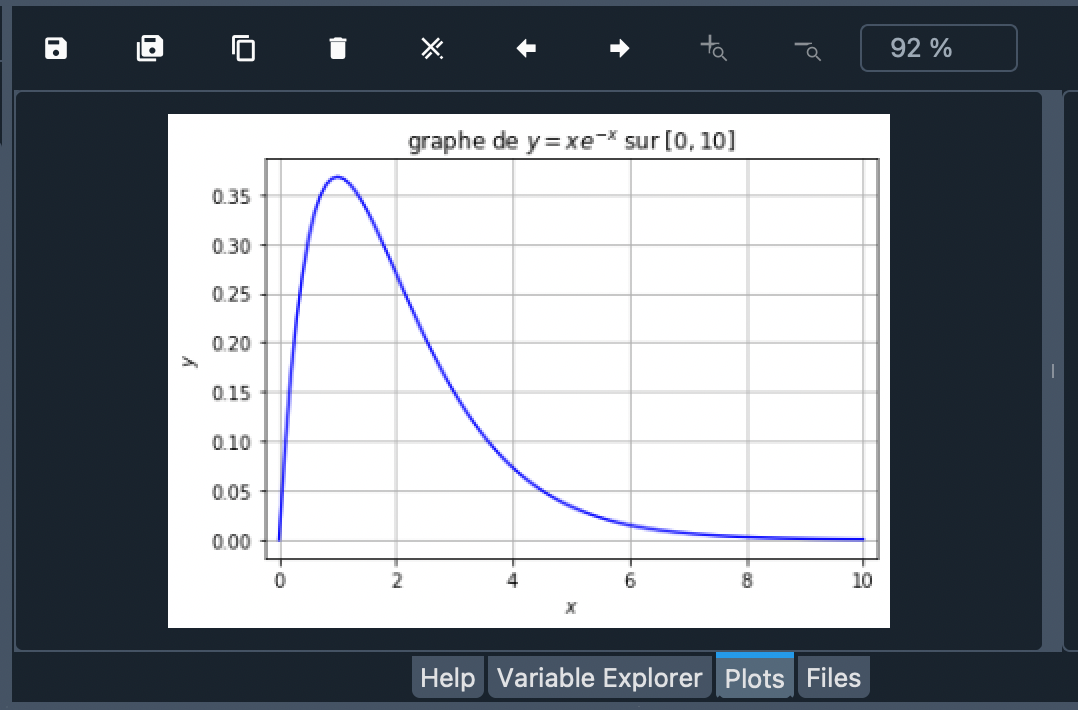
\includegraphics[width=14cm]{./png/plots-courbe.png}
\end{center}
\end{figure}

Les deux vecteurs $x$ et $y$ peuvent être examinés dans le variable explorer. On constate qu'ils sont de type float64 i.e. réels codés sur 64 bits, soit 8 octets.
\begin{figure}[h]
\begin{center}
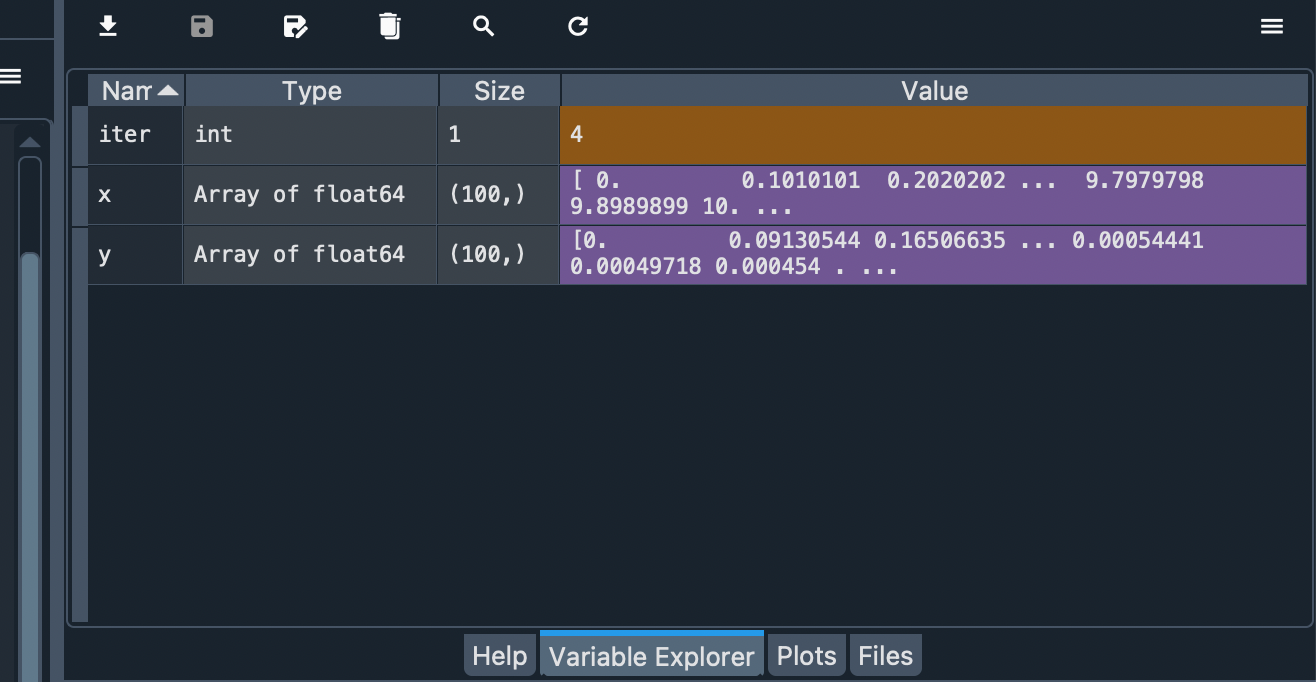
\includegraphics[width=14cm]{./png/variable-explorer-courbe.png}
\end{center}
\end{figure}

La figure obtenue sauvegardée au format png est 
\begin{figure}[h]
\begin{center}
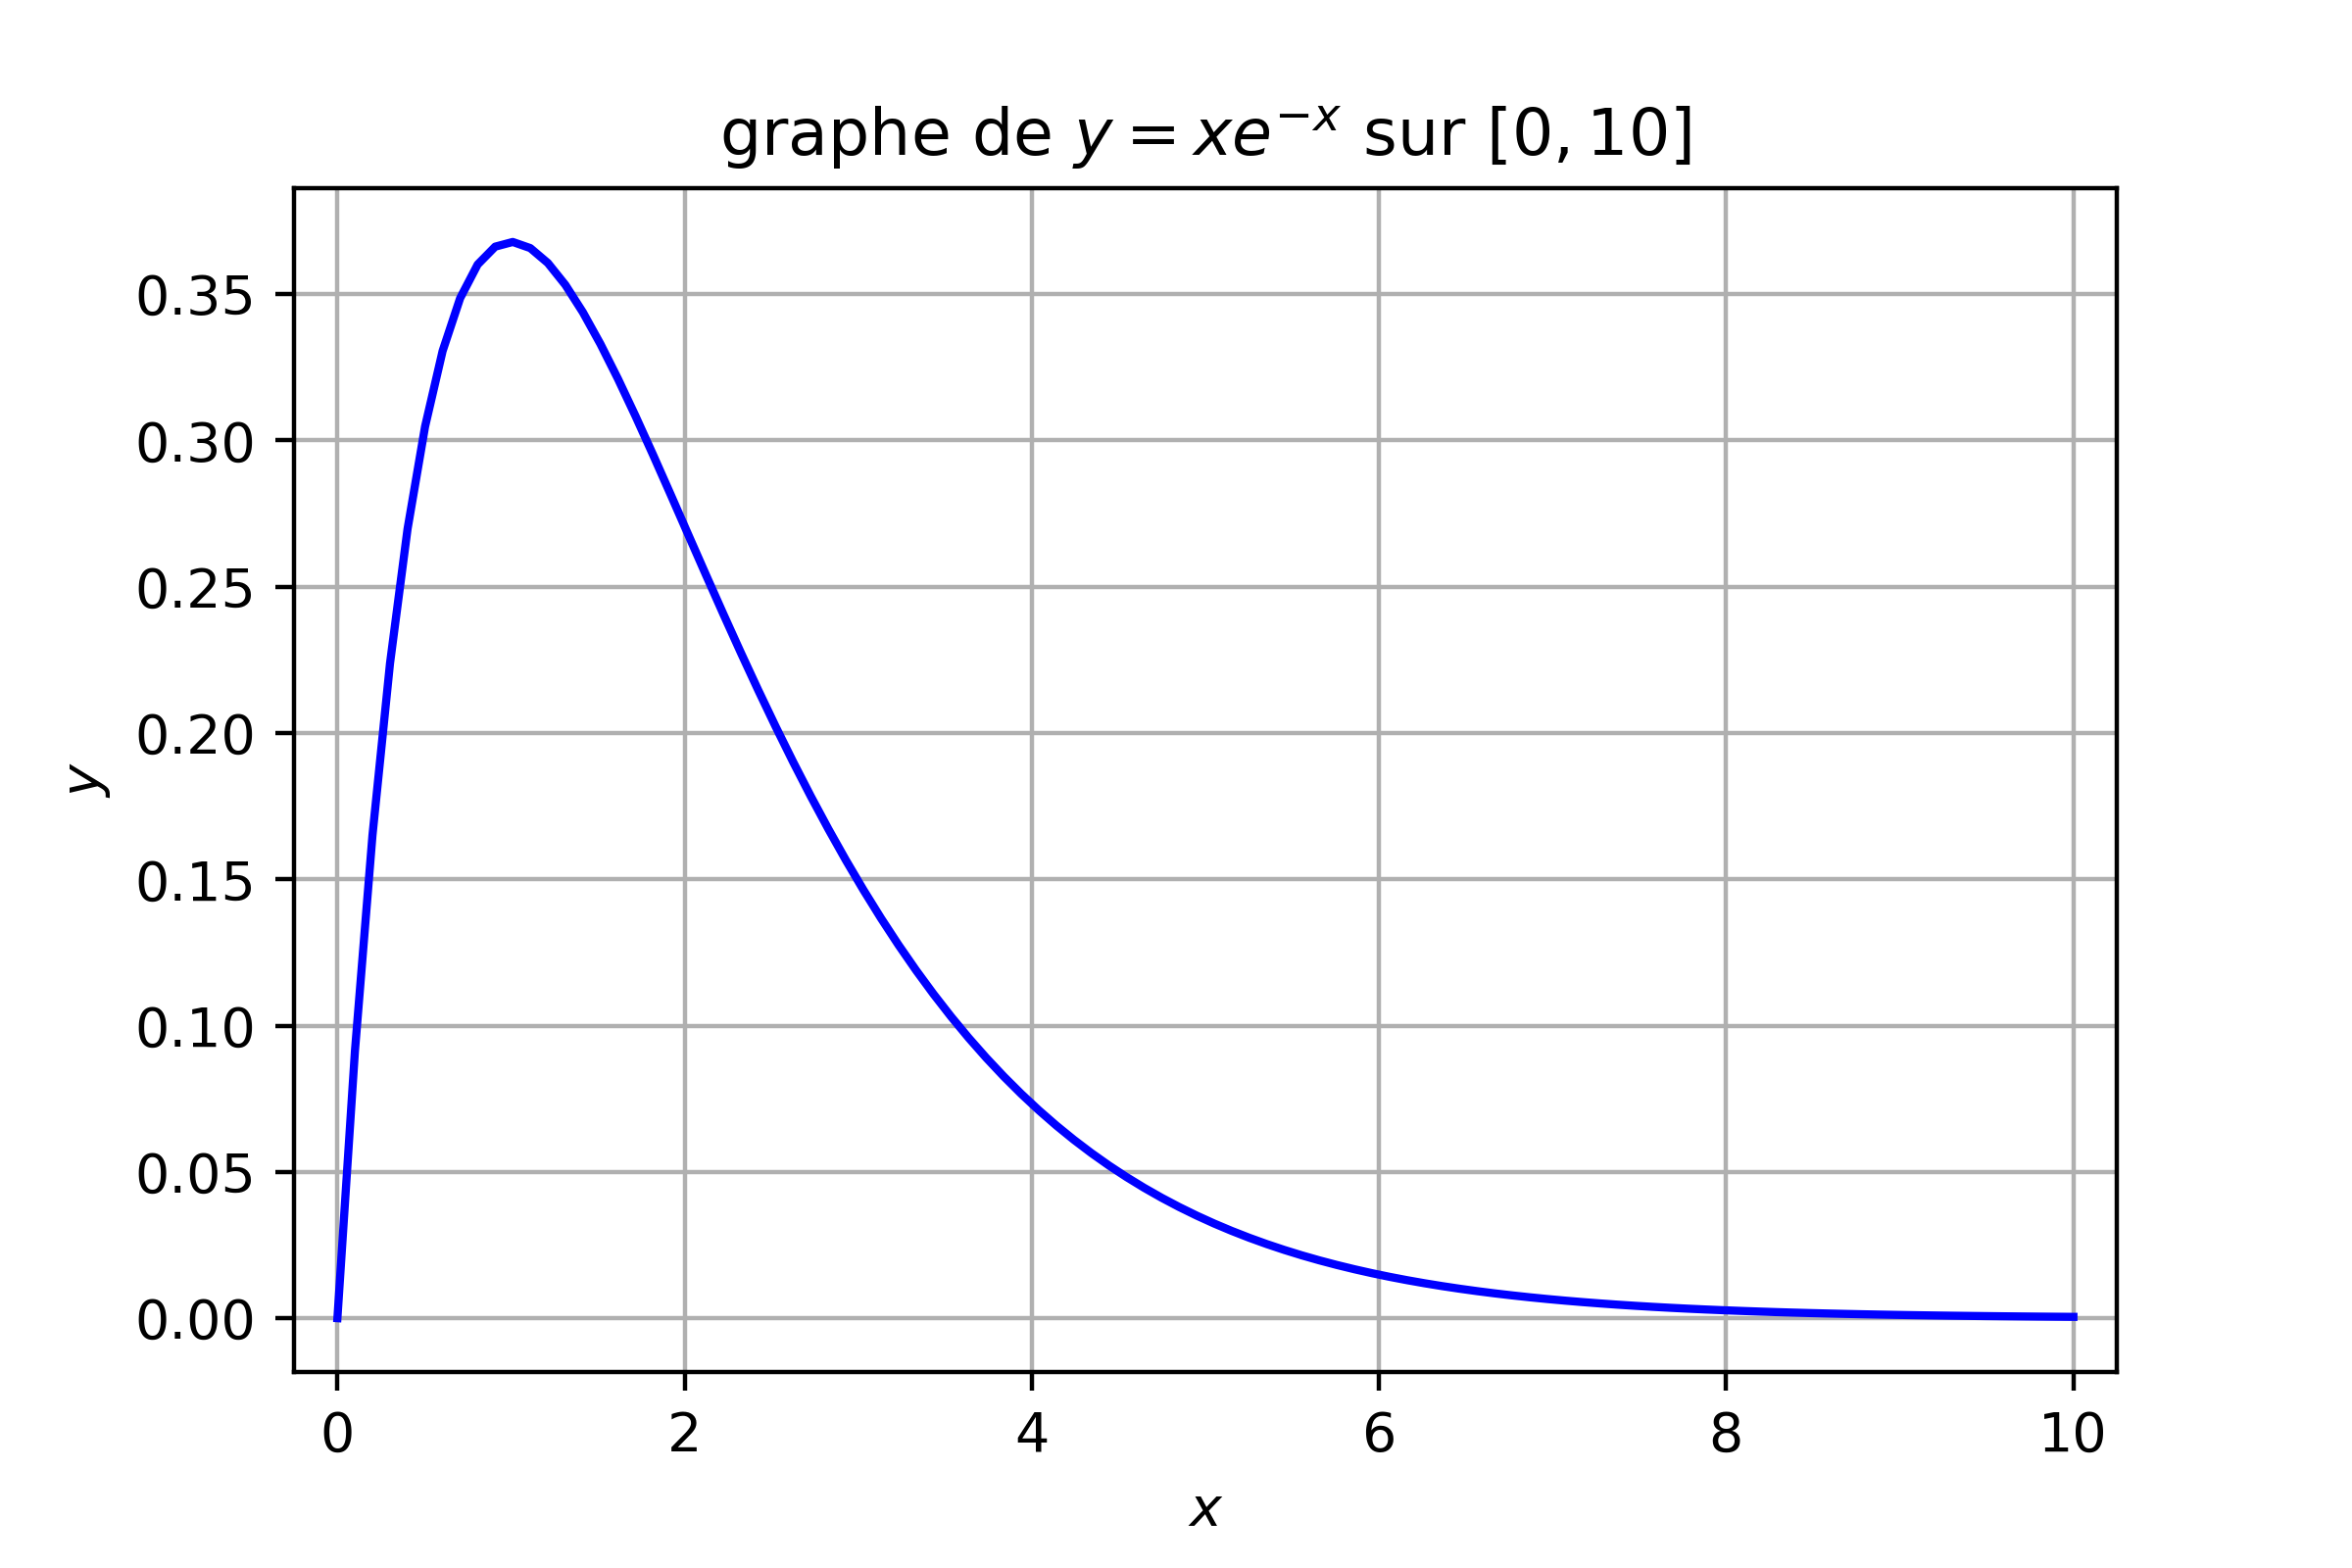
\includegraphics[width=14cm]{./png/expo.png}
\end{center}
\caption{Figure obtenue par le script python et comprenant une légende détaillée.}
\end{figure}

\begin{leftbar}
On veut tracer le nuage de points dont les coordonnées sont sauvegardées dans le fichier \textbf{points.txt} au format deux colonnes, abscisses et ordonnées
\end{leftbar}
\verbatiminput{points.txt}
Le script suivant effectue le tracé.

\lstinputlisting[language=Python]{./codes/plot-points.py} 

L'image obtenue est la suivante
\begin{figure}[h]
\begin{center}
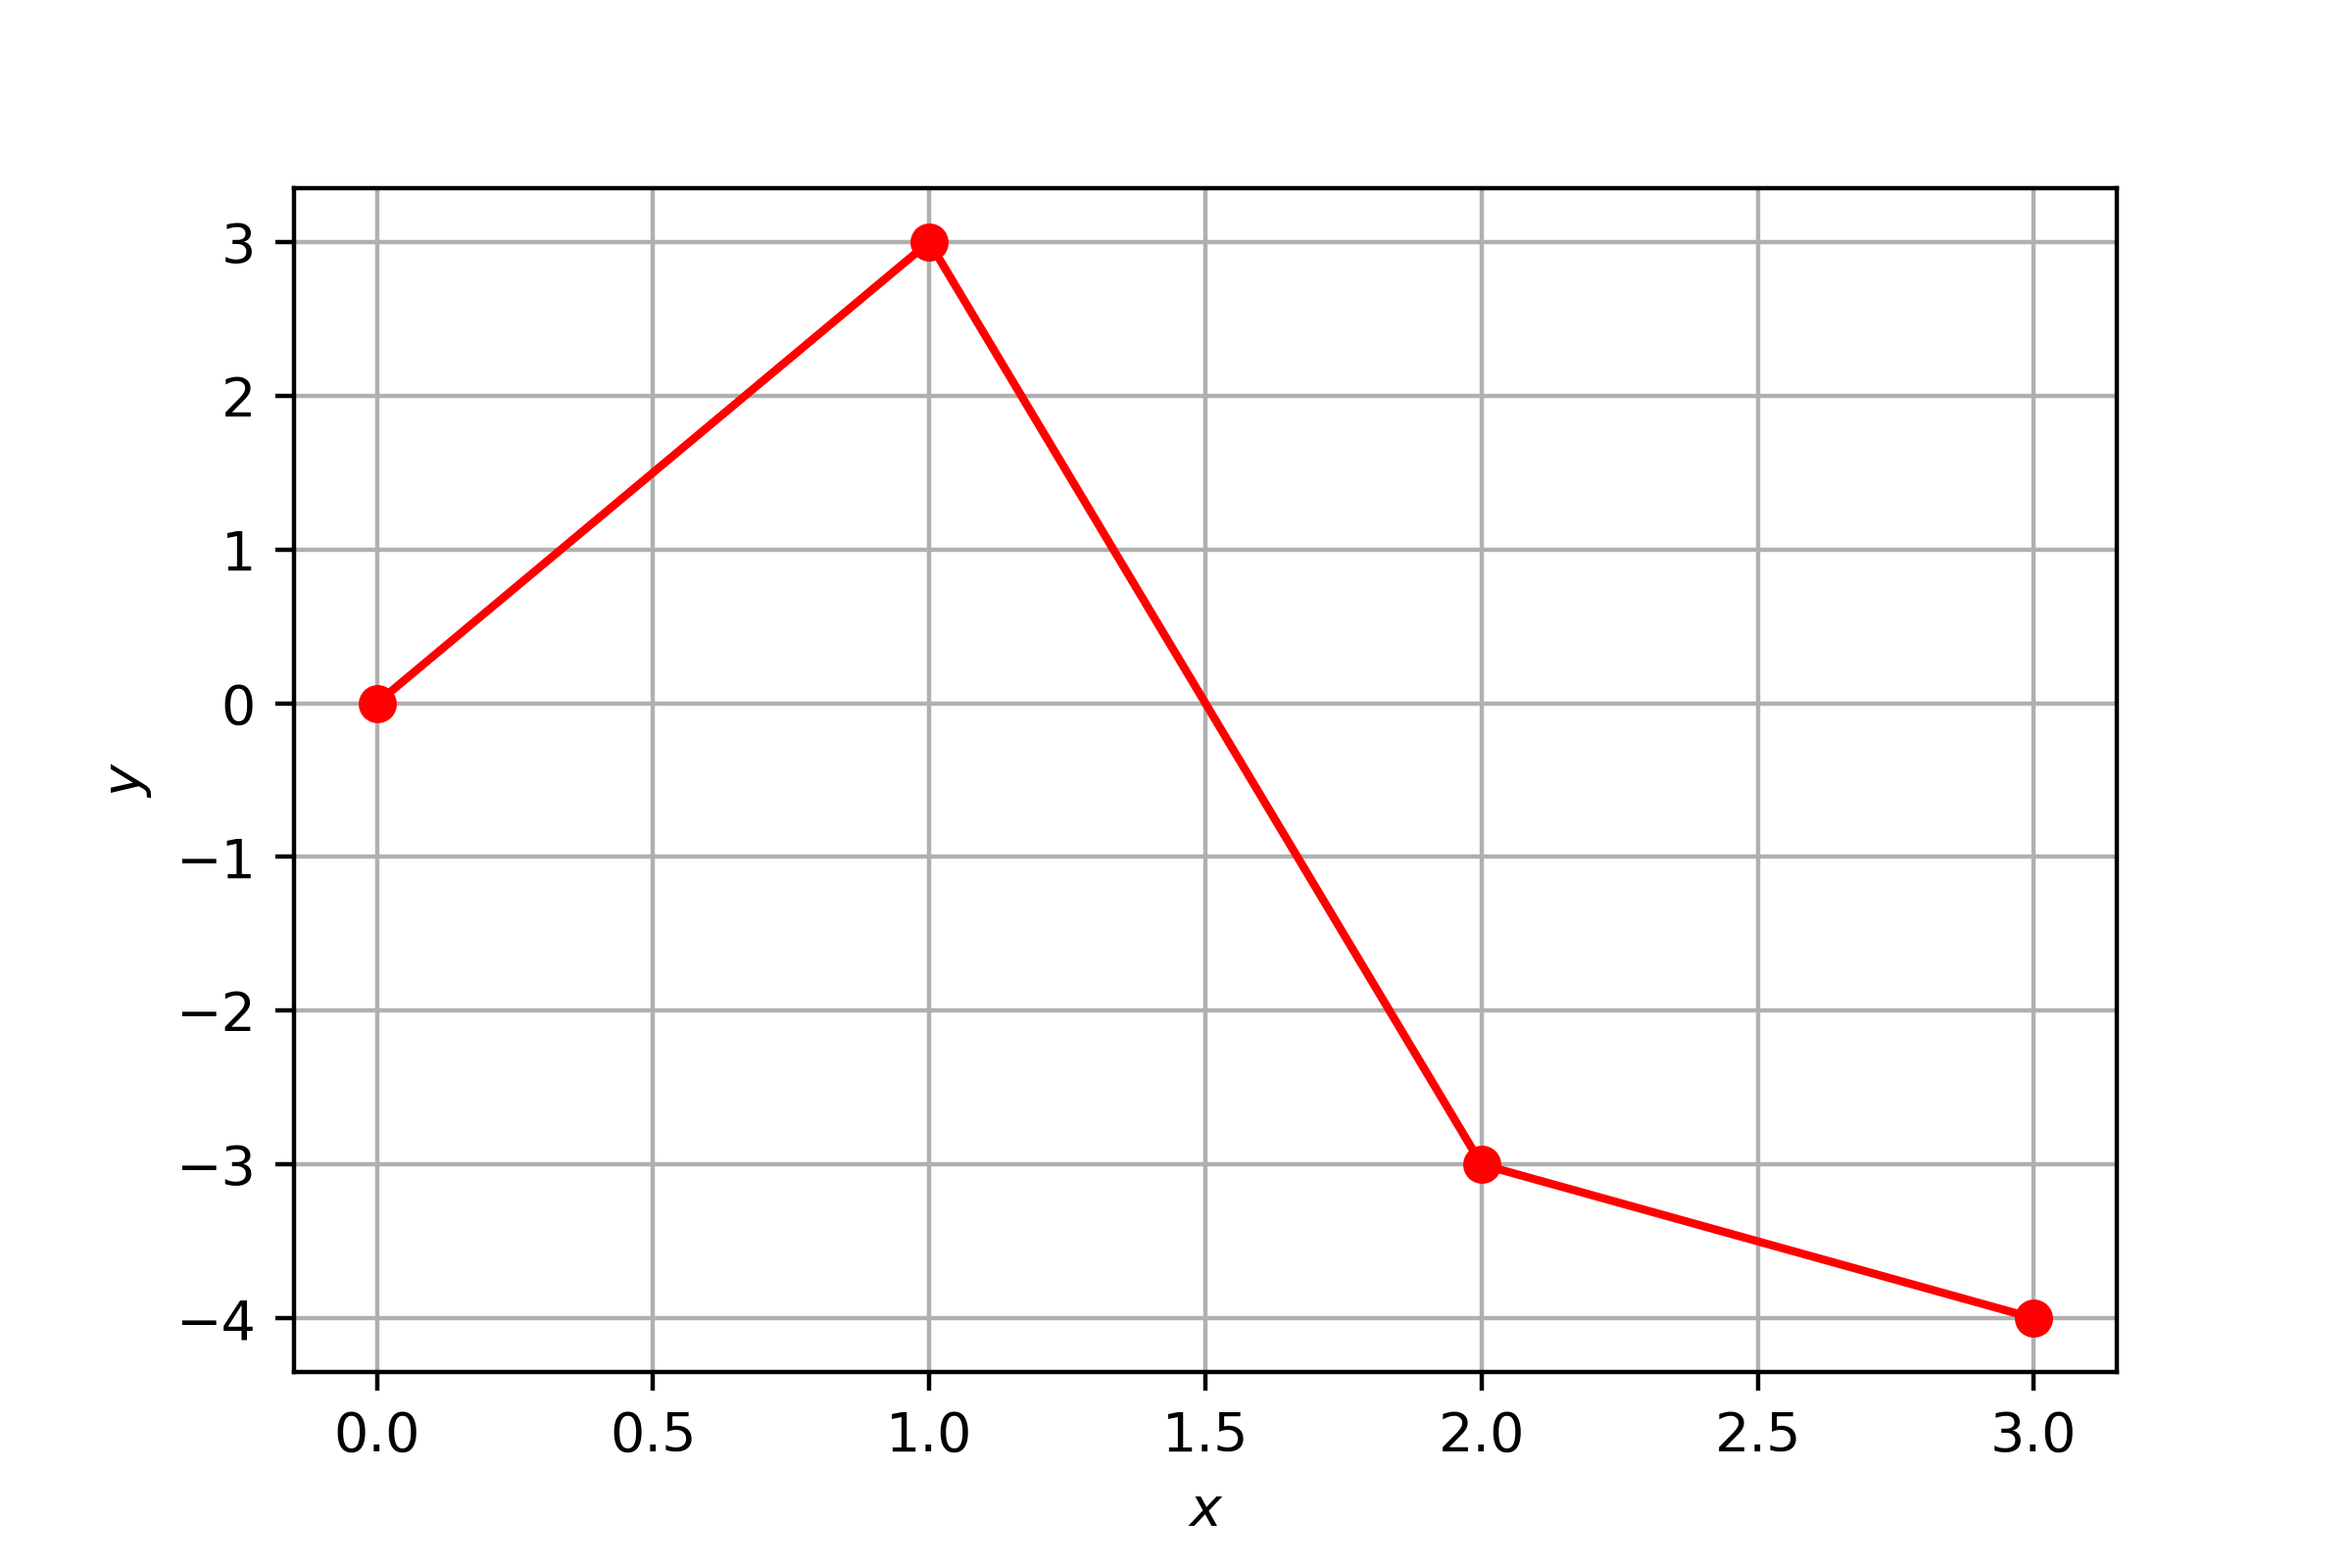
\includegraphics[width=14cm]{./png/points.png}
\end{center}
\caption{Tracé du nuage de points.}
\end{figure}
 
 %-module time
\clearpage
\subsection{time}
\subsubsection{D\'efinition}
Ce module permet de mesurer en secondes le temps écoulé entre deux sections de code. 
\subsubsection{Exemple}
Ce script mesure le temps de calcul pour \'evaluer la somme $\sqrt{1}+\dots+\sqrt{10^6}$.
\begin{lstlisting}[language={Python}]
import time
import math
z=1.0
tic=time.time()
for i in range(10**6):
    z=z+math.sqrt(i)
toc=time.time()
print("duree="+str(toc-tic)+" [s]")
\end{lstlisting}
On obtient le r\'esultat suivant
\begin{verbatim}
duree=0.1428968906402588 [s]
\end{verbatim}
\subsubsection{Exercice}
Ecrire un script python qui mesure le temps pour \'evaluer la somme $1\times 1+\dots+10^6\times 10^6$
\subsubsection{Correction}
Le script suivant peut \^etre propos\'e
\begin{lstlisting}[language={Python}]
import time
import math
z=1.0
tic=time.time()
for i in range(10**6):
    z=z+i*i
toc=time.time()
print("duree="+str(toc-tic)+" [s]")
\end{lstlisting}

\clearpage
\section{Impl\'ementations d'algorithmes}
Un  algorithme est une succession d'opérations nécessitant souvent de réaliser des tests afin de pouvoir choisir la meilleure option. Parfois un algorithme est répétitif ou itératif jusqu'à obtenir la valeur recherchée. Il peut aussi balayer tout ensemble de valeurs afin d'obtenir la réponse recherchée. 
Dans tous les cas un algorithme doit s'arrêter. Il y a deux manières de réaliser de telles boucles, soit utiliser une clause \textbf{tant qu'une condition n'est pas satisfaite} ou une clause \textbf{Pour un certain nombre de valeurs faire un certain nombre d'opérations}. C'est l'objet de cette section.
\subsection{Comparaison entre nombres réels ou entier}
\begin{leftbar}
Le tableau suivant r\'ecapitule la syntaxe employ\'ee pour comparer deux nombres entre eux.
\end{leftbar}
\begin{center}
	\begin{tabular}{|c|c|} \hline
syntaxe Python         &  signification \\ \hline
$==$                 &     \'egal \`a \\ \hline
$!=$                 &     diff\'erent de \\ \hline
    $>$                  &     sup\'erieur \`a \\ \hline
    $>=$                 &     sup\'erieur ou \'egal \`a \\ \hline
    $<$                  &     inf\'erieur \`a \\ \hline
    $<=$                 &     inf\'erieur ou \'egal \`a \\ \hline
    \end{tabular}
\end{center}
\begin{leftbar}
La comparaison de deux nombres renvoie la valeur \textbf{True} si la réponse est positive et \textbf{False} si la réponse est négative. Il s'agit d'un bool\'een. Attention pour le test d'égalité, on utilise le symbole \textbf{==}. Le symbole \textbf{=} correspond à une affectation. Si on tente d'écrire \textbf{2=3}, le message d'erreur sous la forme d'une étoile rouge est affiché.
\end{leftbar}
\begin{figure}[h]
\begin{center}
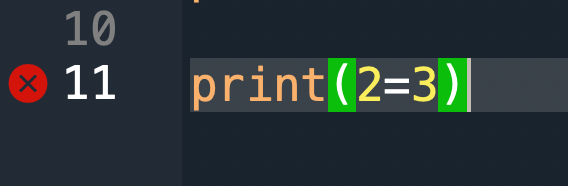
\includegraphics[height=2cm]{./png/erreur.png}
\end{center}
\end{figure}



\lstinputlisting[language=Python]{./codes/test.py}

Le script renvoie les résultats suivants
\begin{verbatim}
False
False
True
True
True
\end{verbatim}

%--
\clearpage
\subsection{Impl\'ementation de la clause Pour}
\begin{leftbar}
Afficher les entiers multiples de 2 et de 3 en utilisant deux tests et la clause pour.
\end{leftbar}

\lstinputlisting[language=Python]{./codes/multiple23.py}

Le script renvoie les résultats suivants
\begin{verbatim}
24 multiple de 2 et 3
30 multiple de 2 et 3
36 multiple de 2 et 3
42 multiple de 2 et 3
48 multiple de 2 et 3
54 multiple de 2 et 3
60 multiple de 2 et 3
66 multiple de 2 et 3\end{verbatim}
 
% Tant que
\clearpage    
\subsection{Impl\'ementation de la clause Tant que }
\begin{leftbar}
Afficher les entiers multiples de 2 et de 3 en utilisant deux tests. On utilisera un compteur que l'on incrémentera (i.e. variable augmentée d'une unité) puis on fera le test.
\end{leftbar}

\lstinputlisting[language=Python]{./codes/compteur.py}

Le script renvoie les résultats suivants
\begin{verbatim}
24 multiple de 2 et 3
30 multiple de 2 et 3
36 multiple de 2 et 3
42 multiple de 2 et 3
48 multiple de 2 et 3
54 multiple de 2 et 3
60 multiple de 2 et 3
66 multiple de 2 et 3
\end{verbatim}
 
\clearpage
%algo iteratif
\subsection{Un exemple d'algorithme it\'eratif}
\begin{leftbar}
On consid\`ere la m\'ethode de H\'eron d'Alexandrie permettant de calculer la racine carr\'ee $\sqrt{a}$ d'un r\'eel $a>0$.
\begin{itemize}
\item[$\bullet$] On veut r\'esoudre l'\'equation
	\[
		x=\frac{1}{2}\left(x+\frac{a}{x}\right)	
	\]
\item[$\bullet$]  par une m\'ethode point fixe qui construit une suite 
	\[
		x_0=a>0\,\quad{}x_{n+1}=f(x_n)	
	\]
\item[$\bullet$]  On programmmera deux m\'ethodes
	\begin{itemize}
	\item l'une utilisant une clause {\textbf{while}}
	\item l'autre utilisant une clause {\textbf{for}}
	\end{itemize}
\item[$\bullet$]  On comptera le nombre d'it\'erations avant convergence.
\item[$\bullet$]  On se donnera un crit\`ere d'erreur $\varepsilon >0$, i.e. on calcule la valeur de $\left|x_{n+1}-\sqrt{a}\right|$.
\item[$\bullet$]  On affichera l'erreur de la m\'ethode \`a chaque it\'eration.
\end{itemize}		
\end{leftbar} 

%--while
\subsubsection{Impl\'ementation avec la clause {\textbf{while}}}

\lstinputlisting[language=Python]{./codes/racine-while.py}
Le r\'esultat du script python

\begin{verbatim}
Recherche racine carree de 2 par methode Heron
methode : clause while

iter= 1  err= 0.08578643762690485  val= 1.5
iter= 2  err= 0.002453104293571373  val= 1.4166666666666665
iter= 3  err= 2.123901414519125e-06  val= 1.4142156862745097
iter= 4  err= 1.5947243525715749e-12  val= 1.4142135623746899
\end{verbatim} 

%%-for
\clearpage
\subsubsection{Impl\'ementation avec la clause {\textbf{for}}}

\begin{leftbar}
Les différence  entre la clause while et la clause for sont les suivantes :
\begin{itemize}
\item pour la clause \textbf{while} on effectue un bloc  d'instructions tant qu'une condition est vérifiée. Le nombre d'exécutions de celles ci n'est pas connues à priori.
\item pour la clause \textbf{for} on exécute  un nombre fixé de fois un bloc  d'instructions. On sort quand la condition demandée est satisfaite par l'instruction \textbf{break}. Cette méthode est préférable à la précédente dans le sens où elle évite à l'algorithme de boucler sans fin. Ceci peut se produire si les paramètres du problème ne sont pas réalistes (par exemple, la valeur du critère de convergence $\epsilon$ est trop faible).
\end{itemize}
\end{leftbar}

\lstinputlisting[language=Python]{./codes/racine-for.py}
Le script permet d'obtenir les résultats suivants
\begin{verbatim}
Recherche racine carree de 2 par methode Heron
methode : clause for

iter= 1  err= 0.08578643762690485  val= 1.5
iter= 2  err= 0.002453104293571373  val= 1.4166666666666665
iter= 3  err= 2.123901414519125e-06  val= 1.4142156862745097
iter= 4  err= 1.5947243525715749e-12  val= 1.4142135623746899
\end{verbatim} 

%--
\clearpage  
\subsection{Cas d'un algorithme r\'ecursif}
\subsubsection{Définition}
\begin{leftbar}
Un algorithme r\'ecursif est d\'efini par une relation de r\'ecurrence et une condition d'arr\^et. En pratique c'est une fonction qui s'appelle elle-m\^eme.
\end{leftbar}
\subsubsection{Exemple}
\begin{leftbar}
La factorielle $n!$ est d\'efinie par la relation de  r\'ecurrence suivante
\begin{equation*}
(n+1)!=(n+1)n!
\end{equation*}
La condition d'arr\^et est la suivante
\begin{equation*}
0!=1
\end{equation*}
\end{leftbar}
\begin{enumerate}
\item On définit une fonction par l'instruction \textbf{def}. L'argument d'entrée est l'entier naturel $n$.
\item On remarque que le type de la variable $n$ n'est pas défini. C'est au programmeur de savoir quel type de variables il manipule.
\item La fonction renvoit le résultat obtenu à l'aide de l'instruction \textbf{return}. Plusieurs résultats peuvent être renvoyés les uns à la suite des autres. On les sépare par le symbole \textbf{,}.
\end{enumerate} 
\begin{lstlisting}[language={Python}]
def fact(n):
    if n==0:
        return 1
    else:
        return n*fact(n-1)

print(fact(5))
print(fact(20))
\end{lstlisting}
Exemple de r\'esultat
\begin{verbatim}
python fact.py 
120
2432902008176640000
\end{verbatim}

%-exercice
\subsubsection{Exercice}
\begin{leftbar}
\begin{enumerate}
\item On demande de calculer le coefficient binomial $\displaystyle\binom{n}{k}$ pour $0\leq k\leq n$ défini par la relation de récurrence valable pour $n\geq 1$
\begin{equation}
\displaystyle\binom{n}{k}=\binom{n-1}{k-1}+\binom{n-1}{k}
\end{equation}
\item On a les relations suivantes $\displaystyle\binom{n}{0}=1$ et $\displaystyle\binom{n}{k}=0$ si $k>n$. 
\item Pour éviter des tests inutiles, on supposera que $k$ et $n$ sont des entiers naturels.
\item On appelera la fonction ainsi définie \textbf{binomrec}.
\end{enumerate}
\end{leftbar}
\subsubsection{Correction}
On a utilisé la fonction \textbf{assert} qui vérifie que la valeur obtenue par la fonction est bien exacte. Si ce n'est pas le cas, un message d'erreur est affiché.
\lstinputlisting[language=Python]{./codes/binomrec.py}

Les résultats suivants sont obtenus par le script.
\begin{verbatim}
k= 11  n= 10  binom= 0
k= 2  n= 5  binom= 10
k= 0  n= 6  binom= 1
\end{verbatim}

\clearpage
\section{Exercices \`a traiter}
%--exercice 1
\subsection{Premier exercice: }
\subsubsection{Enonc\'e}
\begin{leftbar}
Ecrire une fonction \textbf{quad} qui prend en argument trois r\'eels $a$, $b$ et $c$ et qui renvoit le nombre et le valeur des racines r\'eelles suivant l'algorithme suivant et qui les \'ecrive dans un fichier ascii appel\'e quad.txt
\end{leftbar}
\begin{algorithm}
\caption{R\'esolution de $ax^2+bx+c=0$}
\begin{algorithmic}
\State $\Delta\gets b^2-4ac$
\If {$\Delta > 0$}
    \State $r1\gets \displaystyle\frac{-b-\sqrt{\Delta}}{2a}$
    \State $r2\gets \displaystyle\frac{-b+\sqrt{\Delta}}{2a}$
    \State $N \gets 2$
    \newline \textbf{print} $N,\,r1,\, r2$
\ElsIf {$\Delta == 0$}
        \State $r1\gets  \displaystyle\frac{-b}{2a}$
        \State $N \gets 1$
        \newline \textbf{print} $N,\,r1$
\Else
        \State $N \gets 0$
        \newline \textbf{print} $N$
\EndIf
\end{algorithmic}
\end{algorithm}
\clearpage
\subsubsection{Correction}
\lstinputlisting[language=Python]{./codes/quad.py}
Un exemple de r\'esultat
\begin{verbatim}
python quad.py
0
(1, -1.0)
(2, 2.0, 3.0)
\end{verbatim} 
Le fichier quad.txt est de la forme
\begin{verbatim}
0
1 -1.0
2 2.0 3.0
\end{verbatim} 

%--exo 2
\clearpage
\subsection{Second exercice :}
\subsubsection{Enonc\'e}
\begin{leftbar}
\begin{enumerate}
\item On demande de tracer le graphe des fonctions $\cos(x)$, $\sin(x)$ et $\cos(x)+\sin(x)$ sur $[0,2\pi]$ avec 100 points. 
\item On affectera respectivement les couleurs rouge, vert et bleu aux trois courbes. 
\item On sauvegardera les valeurs num\'eriques obtenues dans un fichier nomm\'e 'courbe.dat'.
\end{enumerate}
\end{leftbar}
\subsubsection{Correction}
\lstinputlisting[language=Python]{./codes/trigo.py}

\begin{figure}[h]
\begin{center}
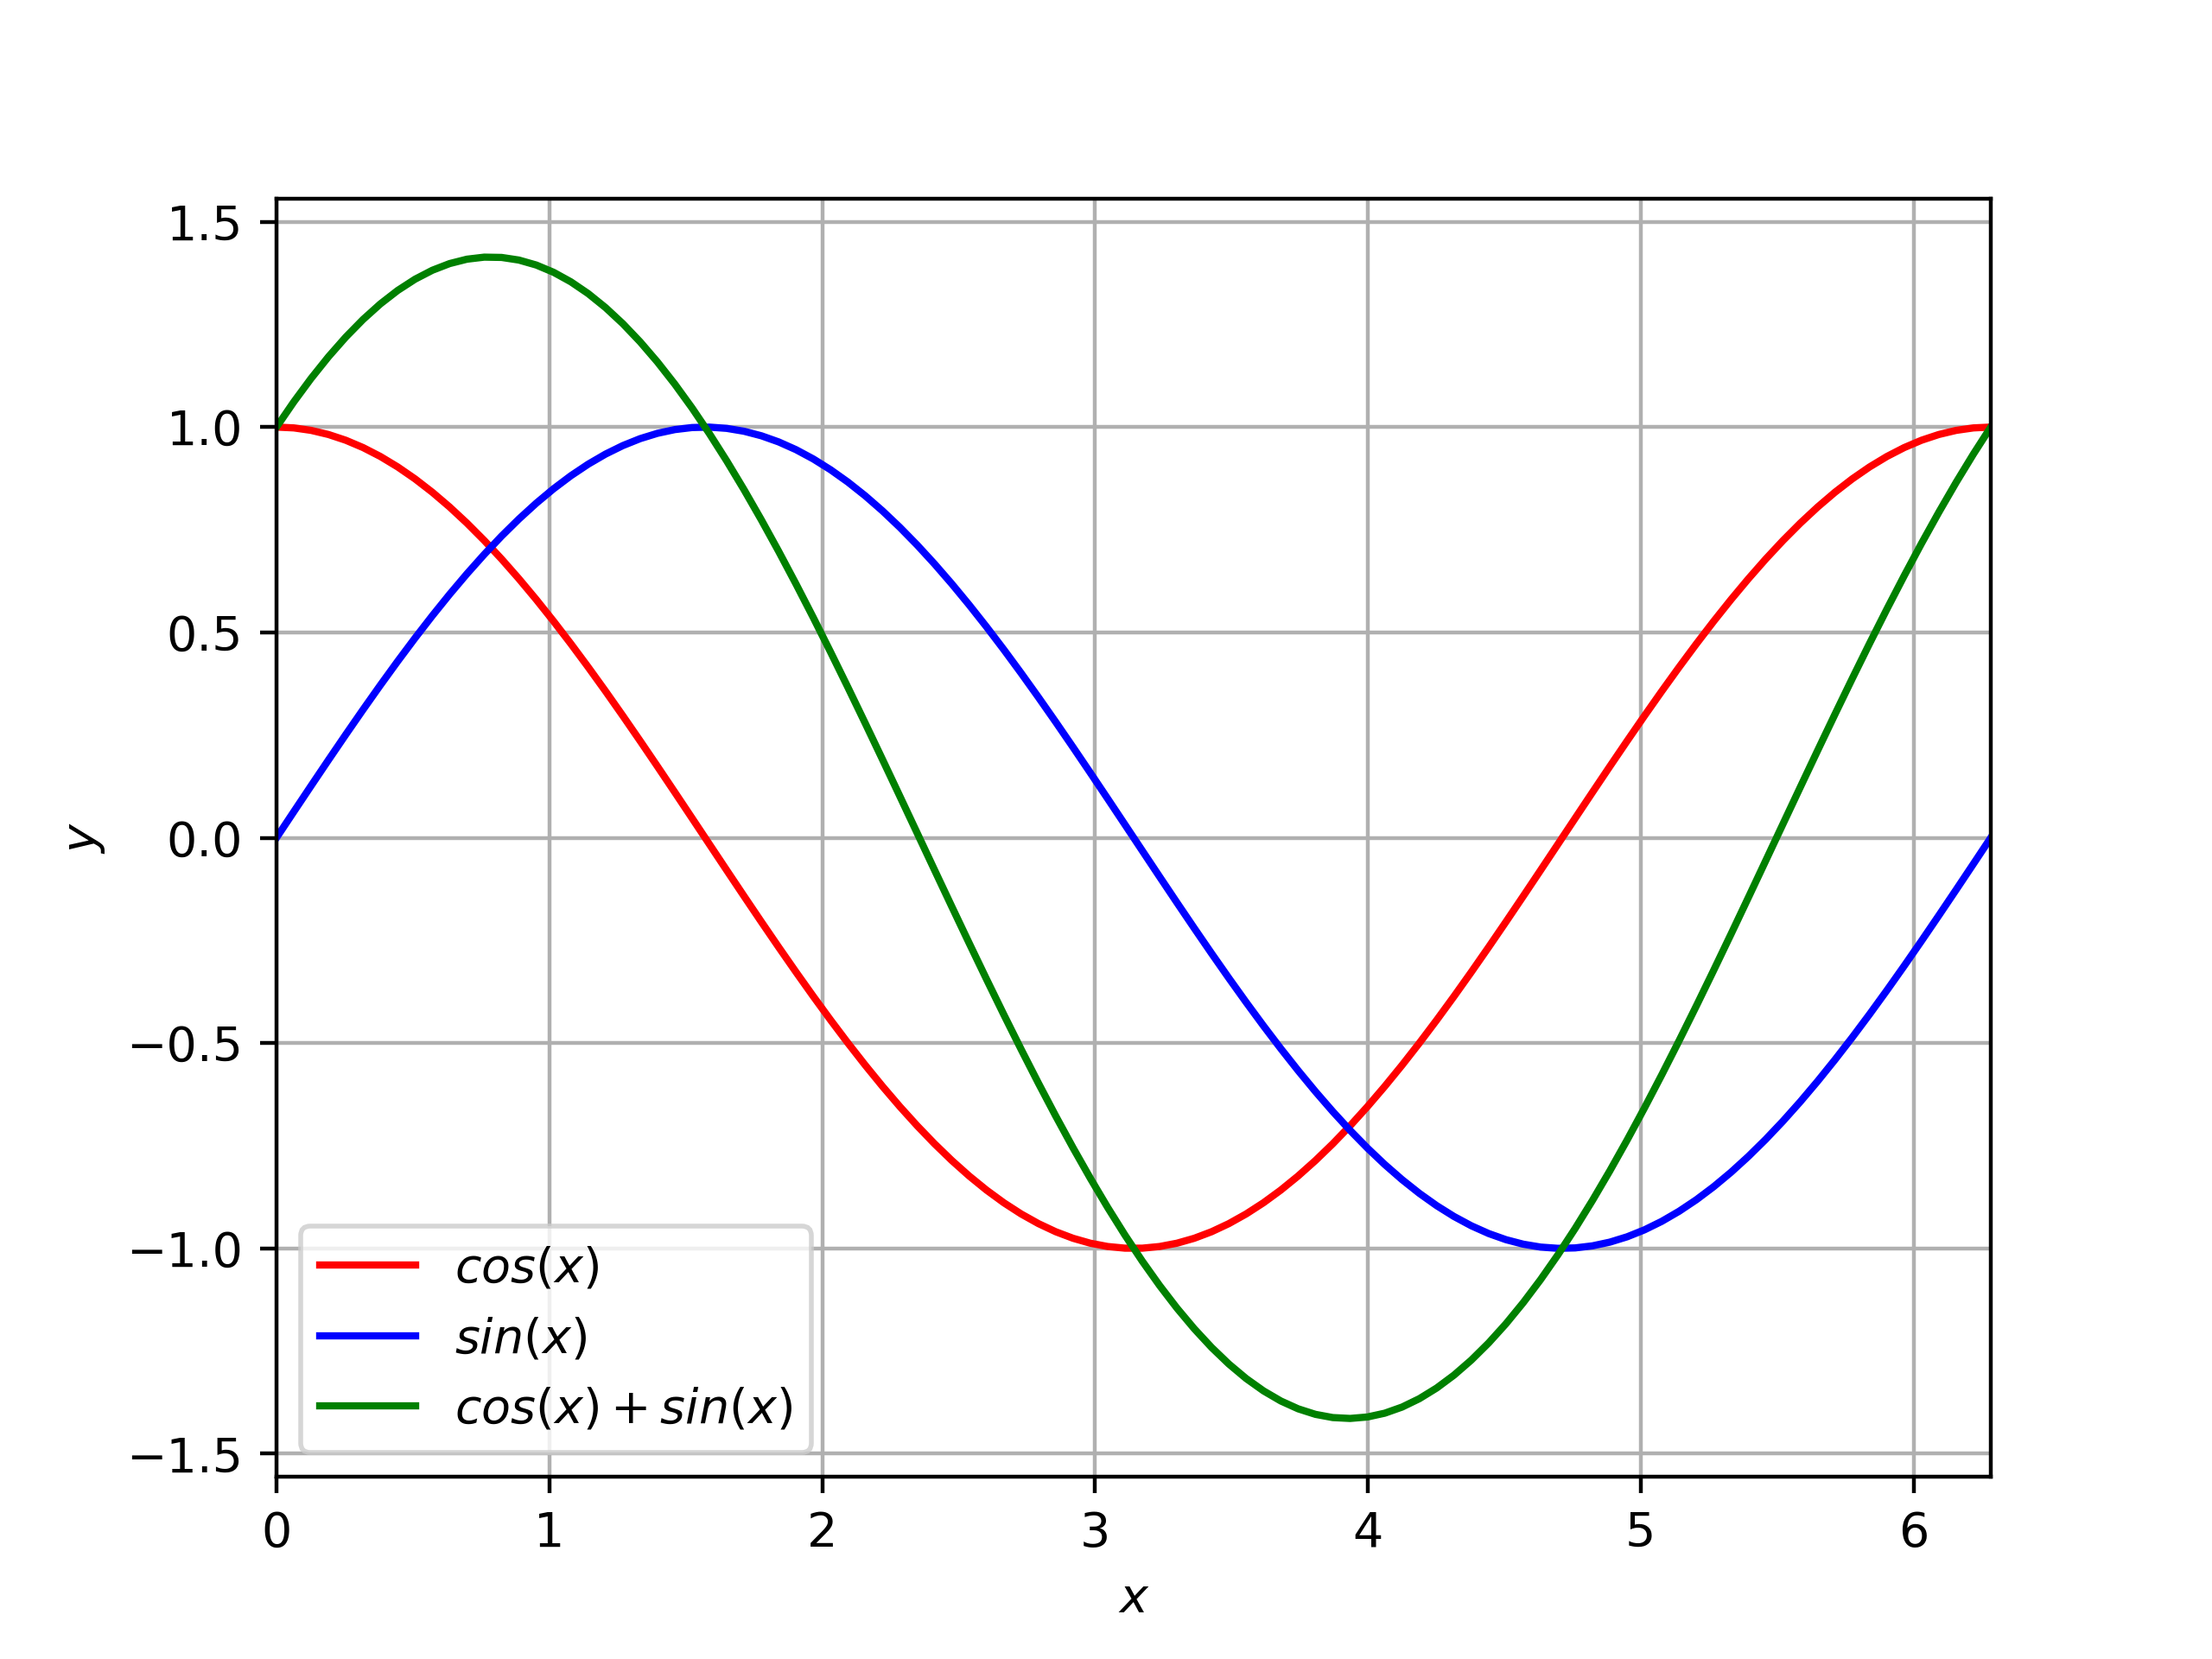
\includegraphics[width=10cm]{./png/trigo}
\end{center}
\caption{Trac\'e des courbes $y=cos(x)$, $y=sin(x)$ et $y=cos(x)+sin(x)$ sur $[0,2\pi]$ avec 100 points.}
\end{figure}

\clearpage
\section{Connaissances \`a ma\^itriser}
Les th\`emes abord\'es lors de l'examen seront les suivants 
\begin{enumerate}
\item Savoir \'ecrire une boucle pour traiter une condition sur des entiers par exemple 
   exemple: etant donn\'e n entier naturel, \'ecrire une fonction qui affiche tous les entiers pairs inf\'erieurs ou \'egaux n

\item Savoir manipuler une liste comprenant des \'el\'ements entiers
   exemple: Programmer la fonction recherche, prenant en param\`etre un tableau non vide tab (type
   list) d'entiers et un entier n, et qui renvoie l'indice de la derni\`ere occurrence de
  l'\'el\'ement cherch\'e. Si l'\'el\'ement n'est pas pr\'esent, la fonction affiche le nombre 0

\item Savoir \'ecrire dans une liste les n premiers termes d'un suite r\'ecurrente donn\'ee par son/ses premiers termes
   exemple: pour la suite u(k+1)=4*u(k) et u(1)=1 et  n=3
   on renvoie [1, 4, 16].

\item Savoir lire un texte \'ecrit sur plusieurs lignes et l'afficher à l'\'ecran

\item Etre capable de compl\'eter un code à trous si le code et l'algorithme sont donn\'es

\item Etre capable d'\'ecrire une fonction programmant un algorithme de tri d'un tableau ayant n \'elements et renvoyer le r\'esultat.

\item Conna\^itre l'usage de la fonction assert pour valider le r\'esultat de certains scripts

\item Savoir manipuler des chaines de caract\`eres: concat\'enation de deux chaines et affichage caract\`ere par caract\`ere.

\item On demande de savoir manipuler la biblioth\`eque numpy et matplotlib.
\end{enumerate}

%--examen 2021
\clearpage
\section{Correction de l'examen de 2021}
%--exo 1
\subsection{Exercice 1}
\begin{leftbar}
Les r\'esultats aux \'evaluations d'un \'el\`eve sont regroup\'es dans une liste compos\'ee de couples (note,coefficient) tels que
\begin{itemize}
\item note est un nombre de type flottant (float) compris entre 0 et 20,
\item coefficient est un nombre entier positif.
\end{itemize}
Ecrire une fonction moyenne qui renvoie la moyenne pond\'er\'ee de cette liste donn\'ee en param\`etre. Par exemple, l'expression moyenne([(15,2),(9,1),(12,3)]) devra renvoyer le r\'esultat du calcul suivant :
\begin{equation*}
\displaystyle\frac{2\times 15+1\times 9+3\times 12}{2+1+3}=12,5
\end{equation*}
\end{leftbar}
Une proposition de correction
\lstinputlisting[language=Python]{./2021/exo1-2021.py}
Un exemple de r\'esultat
\begin{verbatim}
python exo1-2021.py 
75 6
12.5
\end{verbatim}

\clearpage
%-- exo 2
\subsection{Exercice 2}
\begin{leftbar}
\begin{enumerate}
\item On s'int\'eresse \`a la suite d'entiers dite de Fibonacci, d\'efinie par
$u_1=1$, $u_2=1$ et, pour tout entier naturel $n$, par la relation de r\'ecurrence $u_{n+2}=u_{n+1}+u_n$
\item Ecrire la fonction fibonacci \textbf{non r\'ecursive} qui prend un entier $n > 0$ et qui renvoie l'\'el\'ement d'indice $n$ de cette suite.
\item On proposera ensuite une fonction fibonaccisuite qui \'ecrira les 40 premiers termes de la suite de Fibonacci dans un fichier ascii nomm\'e fibo.txt ayant la forme suivante
\begin{verbatim}
1 1
1 1
3 2
4 3
...
\end{verbatim}
\end{enumerate}
\end{leftbar}
Une proposition de correction
\lstinputlisting[language=Python]{./2021/exo2-2021.py}
Un exemple de r\'esultat
\begin{verbatim}
python exo2-2021.py 
1
1
75025
1134903170
\end{verbatim}
\clearpage
\subsection{Exercice 3}
\begin{leftbar}
\begin{enumerate}
\item programmer la fonction recherche, prenant en param\`etre un tableau non vide tab (type list) d'entiers et un entier n, et qui renvoie l'indice de la derni\`ere occurrence de l'\'el\'ement cherch\'e. Si l'\'el\'ement n'est pas pr\'esent, la fonction renvoie la longueur du tableau
\item exemples :
\begin{verbatim}
>>>recherche ([5, 31],1)
2
>>> recherche ([2,4],2)
0
>>> recherche ([2,3,5,2,41],2)
3
\end{verbatim}
\end{enumerate}
\end{leftbar}
Une proposition de correction
\lstinputlisting[language=Python]{./2021/exo3-2021.py}
Un exemple de r\'esultat
\begin{verbatim}
python exo1.py 
liste= [1, 4, 8, 2] resu= 4
liste= [1, 4, 8, 2] resu= 3
\end{verbatim}



%--examen 2022
\clearpage
\section{Correction de l’examen de 2022}
\subsection{Exercice 1}
\begin{leftbar}
On cherche à d\'eterminer les valeurs du triangle de Pascal. Dans ce tableau de forme
triangulaire, chaque ligne commence et se termine par le nombre 1. Par ailleurs, la valeur
qui occupe une case situ\'ee à l’int\'erieur du tableau s’obtient en ajoutant les valeurs des
deux cases situ\'ees juste au-dessus suivant la relation
\begin{equation*}
C(n,k)=C(n-1,k-1)+C(n-1,k)
\end{equation*}
o\`u $0<k<n$
On compl\'etera le script suivant, pour lequel on devra obtenir pour $n = 4$
\begin{verbatim}
>> pascal(4)
[[1], [1, 1], [1, 2, 1], [1, 3, 3, 1], [1, 4, 6, 4, 1]]
\end{verbatim}
Et pour n = 5, voici ce que l’on devra obtenir :
\begin{verbatim}
>> pascal(5)
[[1], [1, 1], [1, 2, 1], [1, 3, 3, 1], [1, 4, 6, 4, 1], [1, 5, 10,
10, 5, 1]]
\end{verbatim}
On devra \'ecrire ensuite une fonction permettant de sauvegarder sur un fichier les valeurs obtenues pour un entier $n$ donn\'e. On doit avoir pour $n=4$
\begin{verbatim}
1
1 1
1 3 3 1
1 4 6 4 1 
\end{verbatim}
\end{leftbar}
\begin{verbatim}
def pascal(n):
    C= [[1]]
    for k in range(1,...):
        Ck = [...]
        for i in range(1,k):
            Ck.append(C[...][i-1]+C[...][...] )
            Ck.append(...)
            C.append(Ck)
     return C
\end{verbatim}
\clearpage
Une proposition de correction
\lstinputlisting[language=Python]{./2022/exo1-2022.py}
Un exemple de r\'esultat
\begin{verbatim}
python exo1-2022.py 
[[1], [1, 1], [1, 2, 1], [1, 3, 3, 1], [1, 4, 6, 4, 1]]
\end{verbatim}
Le fichier cr\'e\'e est 
\begin{verbatim}
1 
1 1 
1 2 1 
1 3 3 1 
1 4 6 4 1 
\end{verbatim}
 


\clearpage
\subsection{Exercice 2}
\begin{leftbar}
\begin{enumerate}
\item On s'int\'eresse \`a la suite d'entiers g\'en\'eralisant la suite dite de Fibonacci, d\'efinie par
$u_1=1$, $u_2=0$, $u_3=2$ $u_4=3$ et, pour tout entier naturel $n$, par la relation de r\'ecurrence $u_{n+4}=3u_{n+3}+2u_{n+2}-4u_{n+1}+7u_n$
\item Ecrire la fonction fibonacci \textbf{non r\'ecursive} qui prend un entier $n > 0$ et qui renvoie l'\'el\'ement d'indice $n$ de cette suite.
\item On proposera ensuite une fonction fibonaccisuite qui \'ecrira les 10 premiers termes de la suite de Fibonacci dans un fichier ascii nomm\'e fibo.txt constitu\'e de deux colonnes
\item On tracera le graphe d'abscisse $n$ et d'ordonn\'ee $F(n)$.
\item \textbf{Bonus} On programmera une version r\'ecursive de l'algorithme. 
\end{enumerate}
\end{leftbar}

Une proposition de correction
\lstinputlisting[language=Python]{./2022/exo2-2022.py}

\begin{figure}
\begin{center}
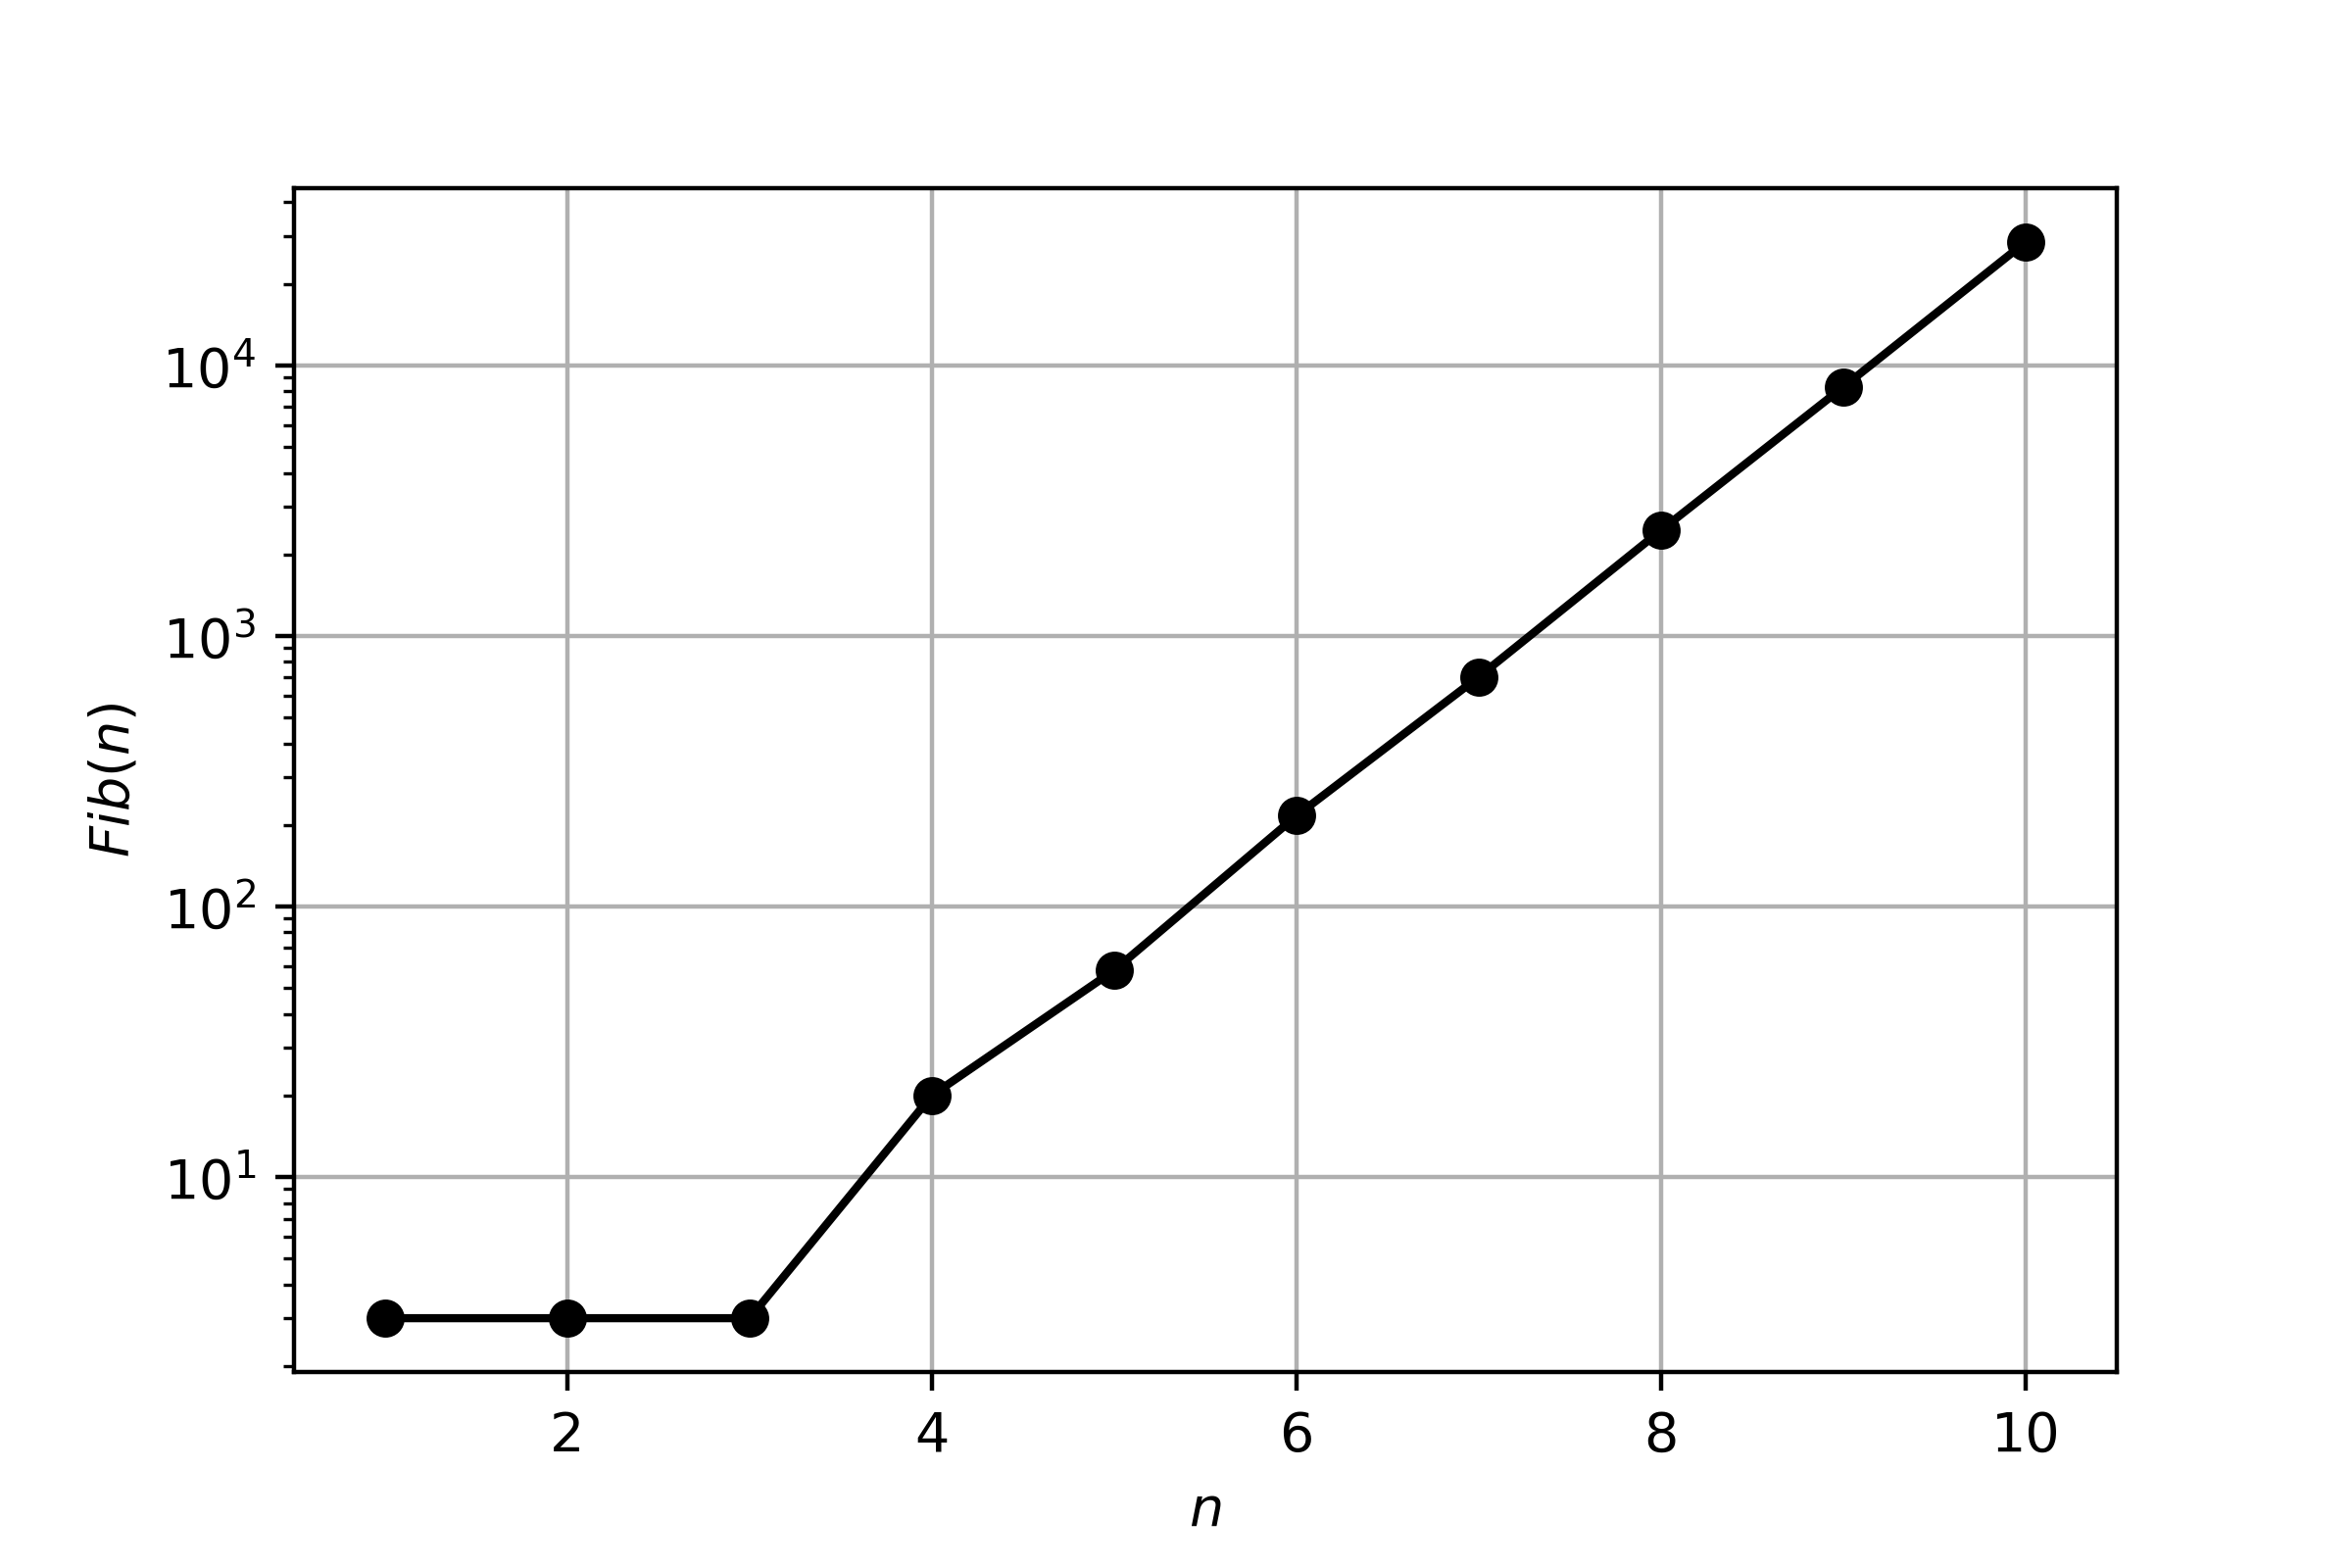
\includegraphics{./2022/fibo.png}
\end{center}
\caption{Evolution de la valeur de $Fib(n)$ en fonction de $n$ en \'echelle log.}
\end{figure}

\clearpage

\subsection{Exercice 3}
\begin{leftbar}
Programmer la fonction verifie qui prend en param\`etre un tableau de valeurs num\'eriques non
vide et qui renvoie True si ce tableau est tri\'e dans l'ordre croissant, False sinon.
\end{leftbar}
\begin{verbatim}
Exemples :
>>> verifie([0, 5, 8, 8, 9])
True
>>> verifie([8, 12, 4])
False
>>> verifie([-1, 4])
True
>>> verifie([5])
True
\end{verbatim}

Une proposition de correction
\lstinputlisting[language=Python]{./2022/exo3-2022.py}
On obtient
\begin{verbatim}
True
False
True
True
\end{verbatim}
\clearpage
\subsection{Exercice 4}
\begin{leftbar}
Etant donn\'ee une liste de r\'eels $[x_1, x_2,\ldots, ...x_n]$, on demande d'\'ecrire un script python calculant

\begin{enumerate}
\item La moyenne $m$ telle que
\begin{equation*}
m=\displaystyle\frac{\sum\limits_{i=1}^n x_i}{n}
\end{equation*}
\item L'\'ecart-type $s$ tel que 
\begin{equation*}
s=\displaystyle\sqrt{\frac{1}{n}\sum_{i=1}^n \left(x_i-m\right)^2}
\end{equation*}
\end{enumerate}
\end{leftbar}
Une proposition de correction
\lstinputlisting[language=Python]{./2022/exo4-2022.py}
On obtient
\begin{verbatim}
notes     = [1, 2, 3]
moyenne   = 2.0
ecart type= 0.816496580927726
\end{verbatim}




\clearpage
%--2023
\section{Correction de l’examen de 2023}
\subsection{Exercice 1}
\begin{leftbar}
On consid\`ere la suite $(u_n)$ telle que 
\begin{eqnarray*}
u_0&=&1\\
u_{n+1}&=&u_n^2+\frac{1}{u_n}+e^{-u_n}
\end{eqnarray*}
On demande d'\'ecrire une fonction python prenant en argument $n$, puis 
\begin{enumerate}
\item calculant $u_n$ par r\'ecurrence, on renverra la valeur de $u_n$ et le temps de calcul.
\item calculant $u_n$ par r\'ecurrence, en optimisant le nombre d'appels r\'ecursifs. on renverra la valeur de $u_n$ et le temps de calcul.
\item calculant $u_n$ sans r\'ecurrence,  on renverra la valeur de $u_n$ et le temps de calcul.
\end{enumerate}
Ces trois fonctions \'etant \'ecrites, on calculera les valeurs de $u_2,\ldots,u_{10}$ puis on tracera l'\'evolution du temps cpu requis par ces trois fonctions en ordonn\'ee et $n$ en abscisse. On pourra utiliser la fonction 
\begin{verbatim}
plt.loglog
\end{verbatim} 
pour tracer en \'echelle loglog. 

On devrait obtenir le graphe suivant. 
\textbf{Pour quelle raison les graphes relatifs \`a la version scalaire et \`a la version r\'ecursive optimis\'ee se superposent-ils ?}
\end{leftbar}
\begin{figure}[htbp]
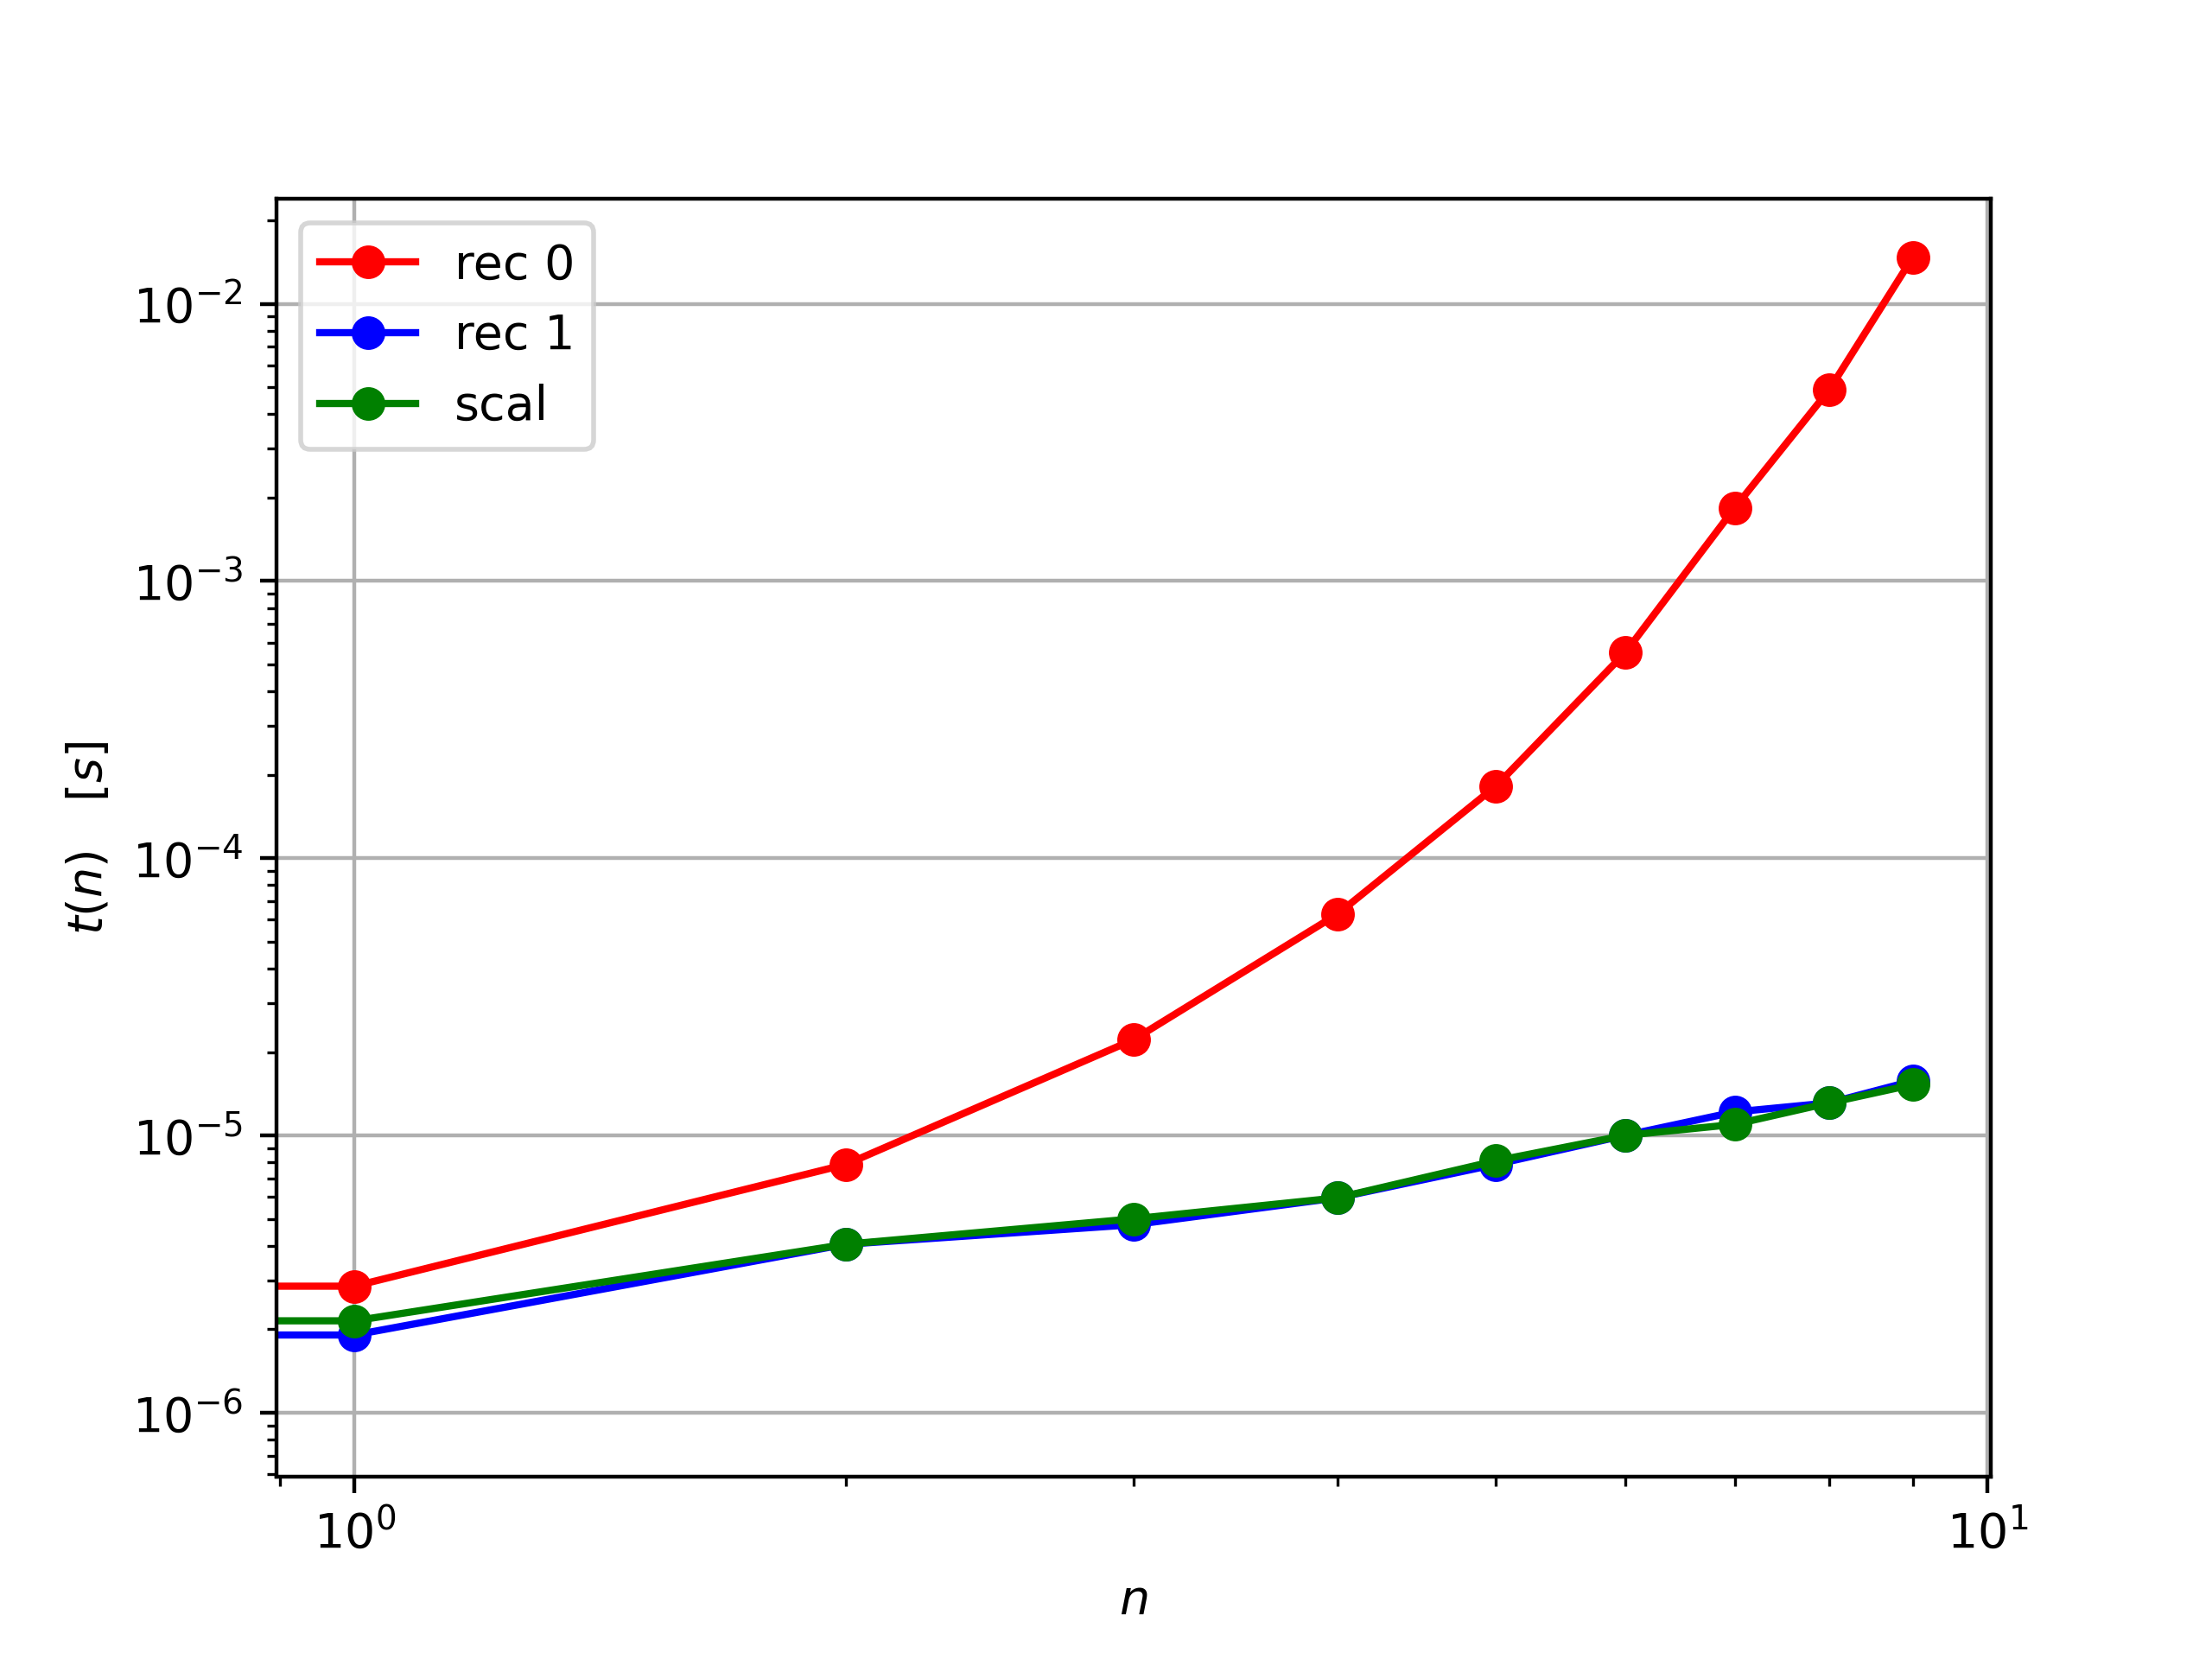
\includegraphics[width=16cm]{./2023/exo1.png}
\end{figure}

Une proposition de correction
\lstinputlisting[language=Python]{./2023/exo1.py}

\clearpage
\subsection{Exercice 2}
\begin{leftbar}
On consid\'ere deux listes $a=[a_0,\ldots,a_n]$ et $b=[b_0,\ldots,b_p]$ ayant respectivement $n+1$ et $p+1$ \'el\'ements. On demande d'\'ecrire une  fonction prenant $a$ et $b$ en argument et 
\begin{enumerate}
\item construisant 
\begin{enumerate}
\item la liste $l=[a_0,b_0,\ldots,a_n,b_n]$ si $n\leq p$
\item la liste $l=[a_0,b_0,\ldots,a_p,b_p]$ si $p\leq n$
\end{enumerate}
\item calculant le $\min$, le $\max$ et $\mathrm{moy}$, la moyenne arithm\'etique de la liste $l$
\end{enumerate}
la fonction renverra $l,\min,\max,\mathrm{moy}$. On testera la fonction avec $a=[0,1,2,7]$ et $b=[4,9]$.
\end{leftbar}

Une proposition de correction
\lstinputlisting[language=Python]{./2023/exo2.py}

L'ex\'ecution du script donne le r\'esultat suivant
\begin{verbatim}
python3 exo2.py 
l1 = [0, 1, 2, 7]
l2 = [4, 9]
2
min= 0
max= 9
moy= 3.5
lis= [0, 4, 1, 9]
\end{verbatim}

\clearpage
\subsection{Exercice 3}
\begin{leftbar}
Le chiffre de C\'esar transforme un message en d\'ecalant chaque lettre de celui-ci dans l’alphabet.
Par exemple, avec un décalage de 3, le A se transforme en D, le B en E, ..., le X en A, le Y en B et le Z en C. Les autres caractères (espace ou caract\`ere de ponctuation : ‘!’,’ ?’...) ne sont pas codés. Le d\'ecalage peut \^etre positif vers la droite ou n\'egatif vers la gauche.
La fonction positionalphabet ci-dessous prend donc en param\`etre un caract\`ere lettre et renvoie la position de lettre dans la chaîne de caract\`eres ALPHABET s’il s’y trouve.
La fonction cesar prend en param\`etre une chaîne de caract\`eres message et un nombre entier decalage et renvoie le nouveau message cod\'e avec le codage de C\'esar utilisant le d\'ecalage de valeur decalage.
\begin{verbatim}
 ALPHABET = 'ABCDEFGHIJKLMNOPQRSTUVWXYZ'
def position_alphabet(lettre):
    return ord(lettre) - ord('A')
def cesar(message, decalage):
    resultat = ''
    for c in message:
        d=c.upper()
        if 'A' <= ... and ... <= 'Z':
            indice = (...) \% ...
            resultat = resultat + ALPHABET[indice]
        else:
            resultat = resultat + ...
    return resultat

print(cesar('PHARMACIEN EXPERT EN PYTHON',7))
print(cesar('WOHYTHJPLU LEWLYA LU WFAOVU',-7))
\end{verbatim}    
Compléter la fonction cesar.
\\
R\'esultat
\begin{verbatim}
>>> print(cesar('PHARMACIEN EXPERT EN PYTHON',7))
'WOHYTHJPLU LEWLYA LU WFAOVU'
>>> print(cesar('WOHYTHJPLU LEWLYA LU WFAOVU',-7))
'PHARMACIEN EXPERT EN PYTHON'
\end{verbatim}
\end{leftbar}

Une proposition de correction
\lstinputlisting[language=Python]{./2023/cesar.py}


\clearpage
\subsection{Exercice 4}
\begin{leftbar}
On se donne une liste $l$ ayant un nombre pair $n$ \'el\'ements, constitu\'ee de $n$  \'el\`eves de l'option pharmacie. Ils seront r\'epartis al\'eatoirement dans deux sous listes de taille $\frac{n}{2}$ . Chacune de ces deux sous-listes contiendra donc le nom des \'el\`eves choisis al\'eatoirement. On demande d'\'ecrire un tel script qui prend en argument la liste $l$ et renvoie les deux sous-listes $l1$ et $l2$ cr\'e\'ees. On utilisera la biblioth\`eque random qui g\'en\'erera les entiers al\'eatoires requis pour choisir l'affectation vers la liste $l1$ ou la liste $l2$.
 \end{leftbar}
 R\'esultat
\begin{verbatim}
liste=["a","b","c","d","e","f"]
ll1,l2=pharma(liste)
print("l1=",l1)
print("l2=",l2)
l1= [['a'], ['c'], ['d']]
l2= [['b'], ['e'], ['f']]

liste=["a","b","c","d","e","f"]
l1,l2=pharma(liste)
print("l1=",l1)
print("l2=",l2)
l1= [['c'], ['d'], ['e']]
l2= [['a'], ['b'], ['f']]

liste=["a","b","c","d","e","f"]
l1,l2=pharma(liste)
print("l1=",l1)
print("l2=",l2)
l1= [['a'], ['b'], ['d']]
l2= [['c'], ['e'], ['f']]
\end{verbatim}

Une proposition de correction
\lstinputlisting[language=Python]{./2023/pharma.py}


\clearpage
%--2024
\section{Correction de l’examen de 2024}
\subsection{Exercice 1}
\begin{leftbar}
On souhaite calculer une approximation de $\pi$ par la formule 
\begin{itemize}
\item de Vi\`ete telle qu'au rang $n$
\begin{equation*}
\pi_n^V=\frac{2\times 2^n}{u_0\times u_1\times u_2\ldots u_n}
\end{equation*}
o\`u 
\begin{eqnarray*}
u_0&=&\sqrt{2}\\ \nonumber
u_{k+1}&=&\sqrt{2+u_k}
\end{eqnarray*}
\item la formule de Gr\'egory telle qu'au rang $n$
\begin{equation*}
\pi_n^G=\sum_{k=0}^n\frac{4\times(-1)^k}{2k+1}
\end{equation*}
\end{itemize}
On demande d'\'ecrire les fonctions Python suivantes prenant en argument $n$, puis 
\begin{enumerate}
\item calculant l'approximation au rang $n$ de $\pi_n^V$ par la formule de Vi\`ete. On appelera cette fonction $viete(n)$
\item  calculant l'approximation au rang $n$ de $\pi_n^V$ par la formule de Gr\'egory. On appelera cette fonction $gregs(n)$ en utilisant une sipmle boucle. On proposera une autre solution utilisant un algorithme r\'ecursif tel que 
\begin{equation*}
g(n)=4\times\frac{(-1)^n}{2n+1}+g(n-1)
\end{equation*} avec $g(0)=4$. On appelera cette fonction $gregr(n)$ 
\item On tracera l'\'evolution de $gregr(n)$ en fonction de $n\in[1,100]$ ainsi que son temps de calcul sur deux figures distinctes. On fera de m\^eme avec $viete(n)$ 
\end{enumerate}
On devrait obtenir les graphes suivants pour $gregr(n)$ . 
\end{leftbar}
\begin{figure}[htbp]
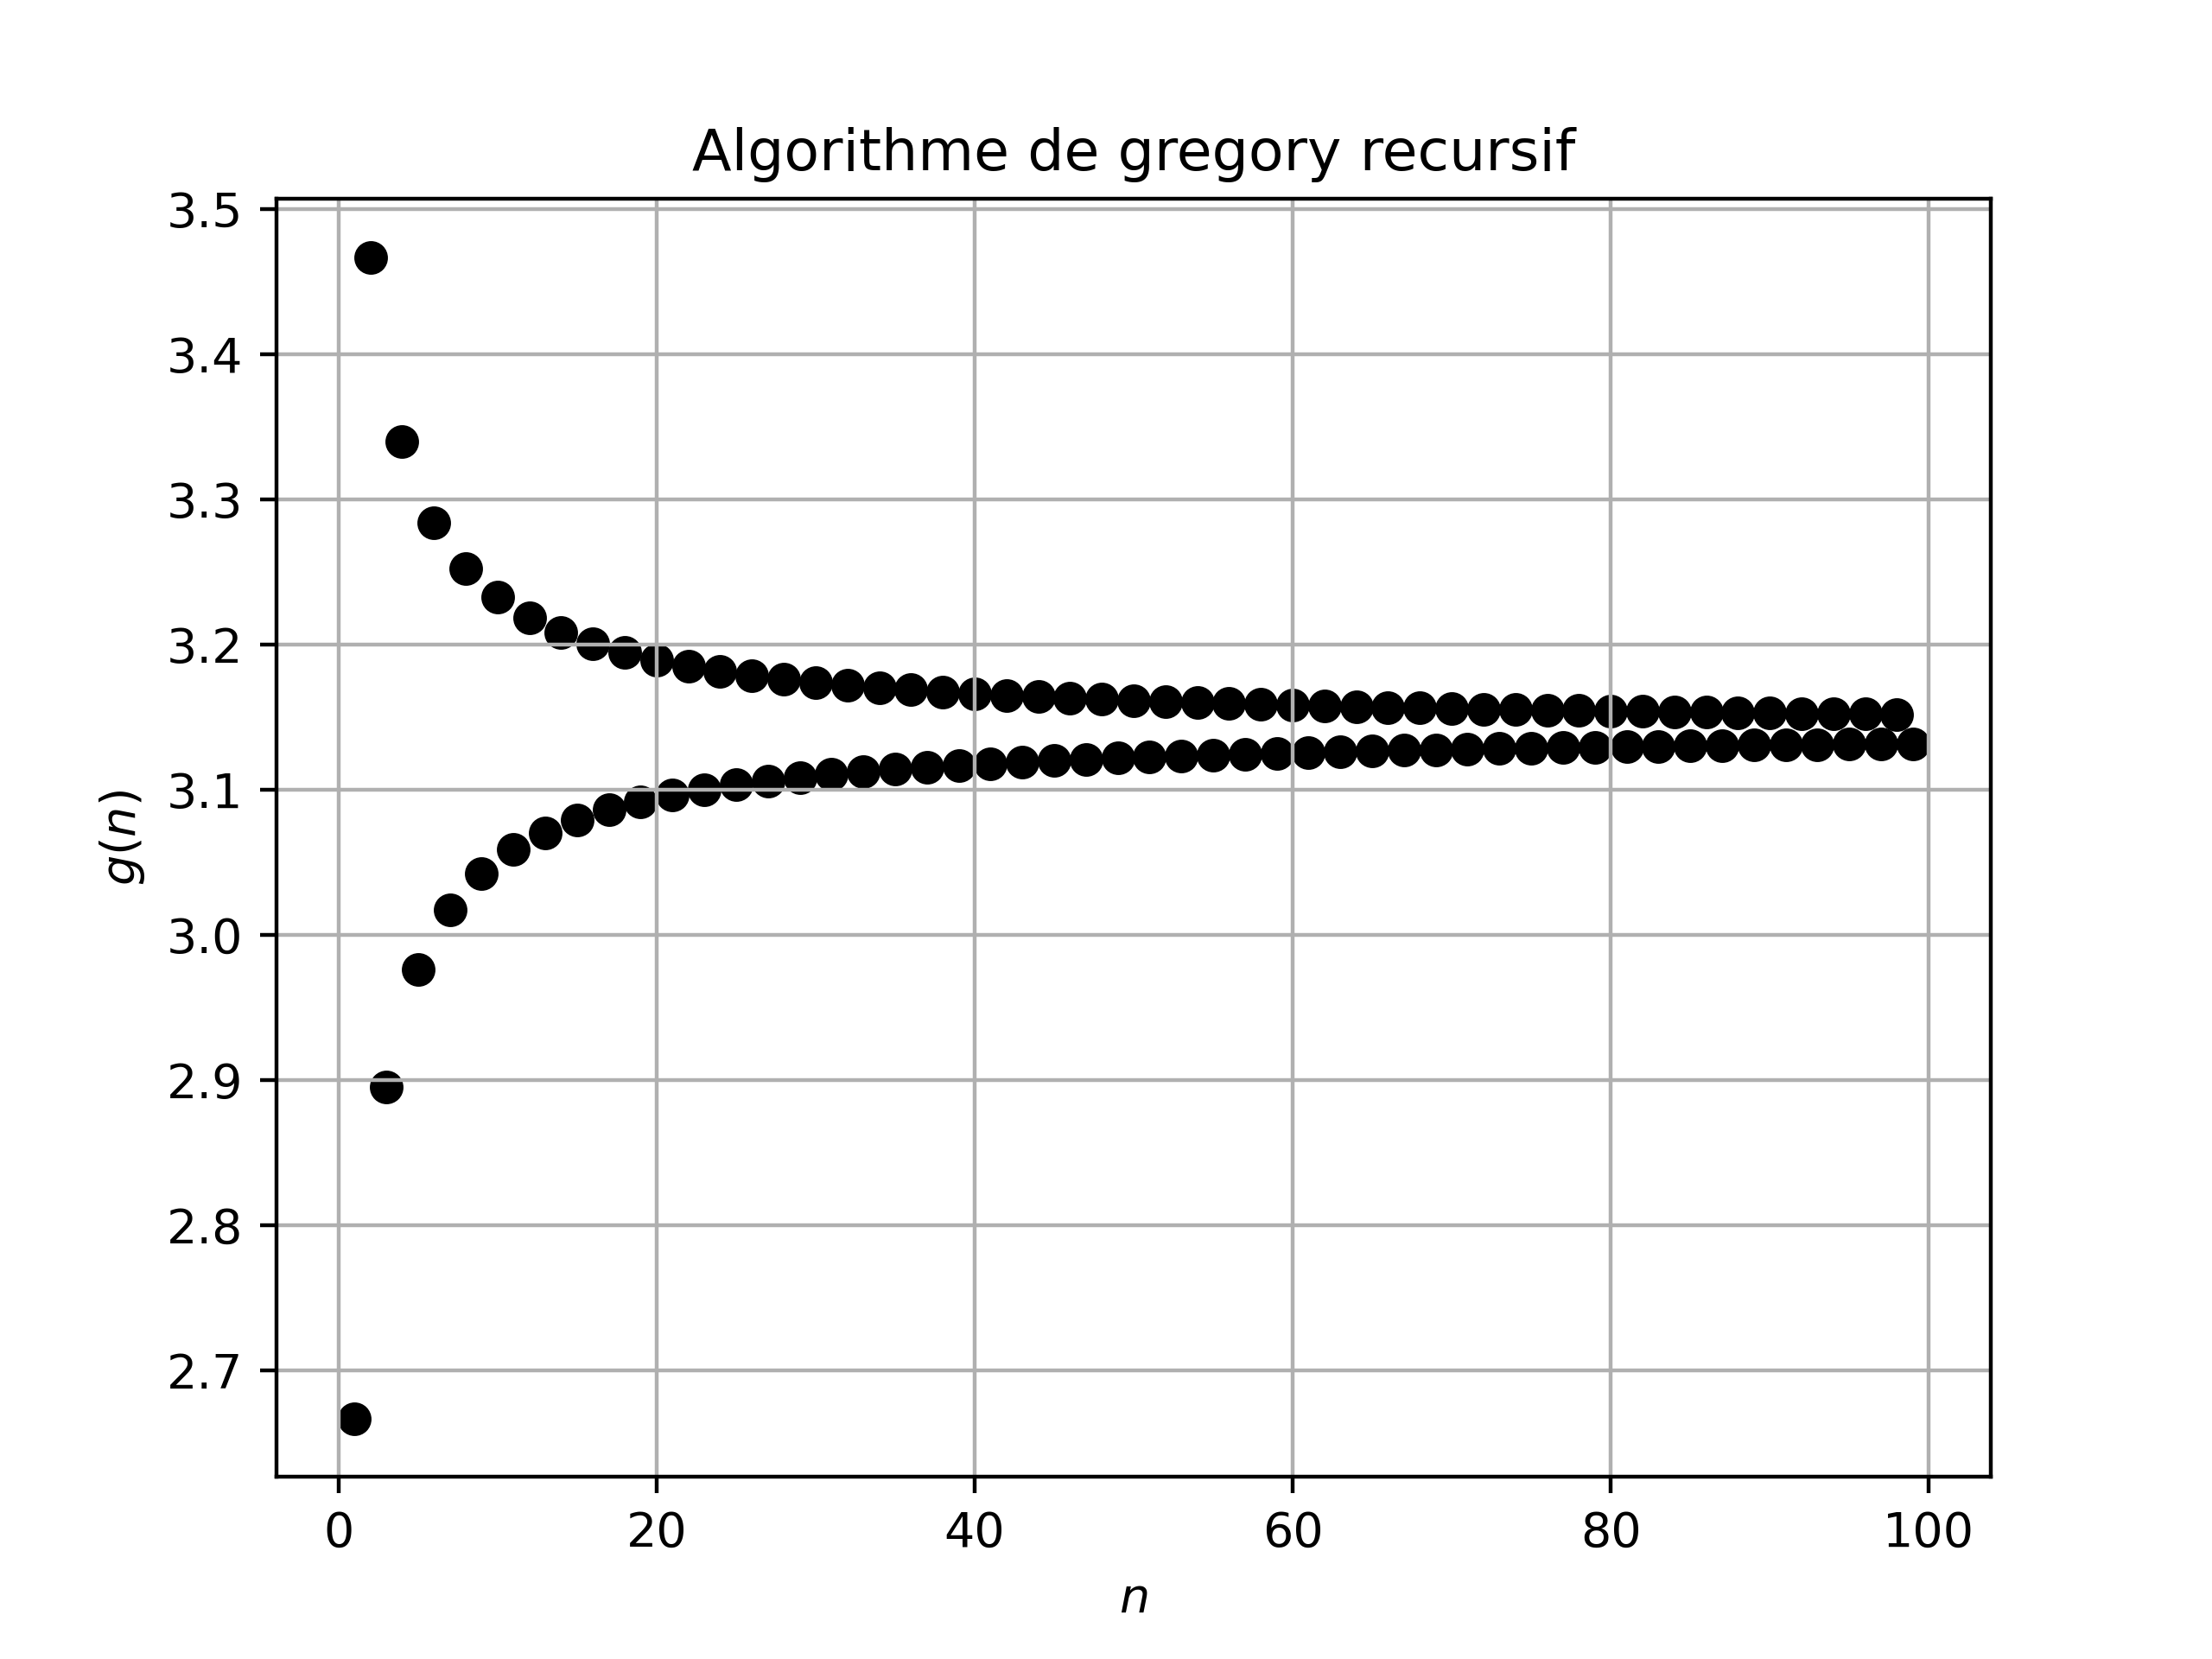
\includegraphics[width=8cm]{./2024/greg-val.png}
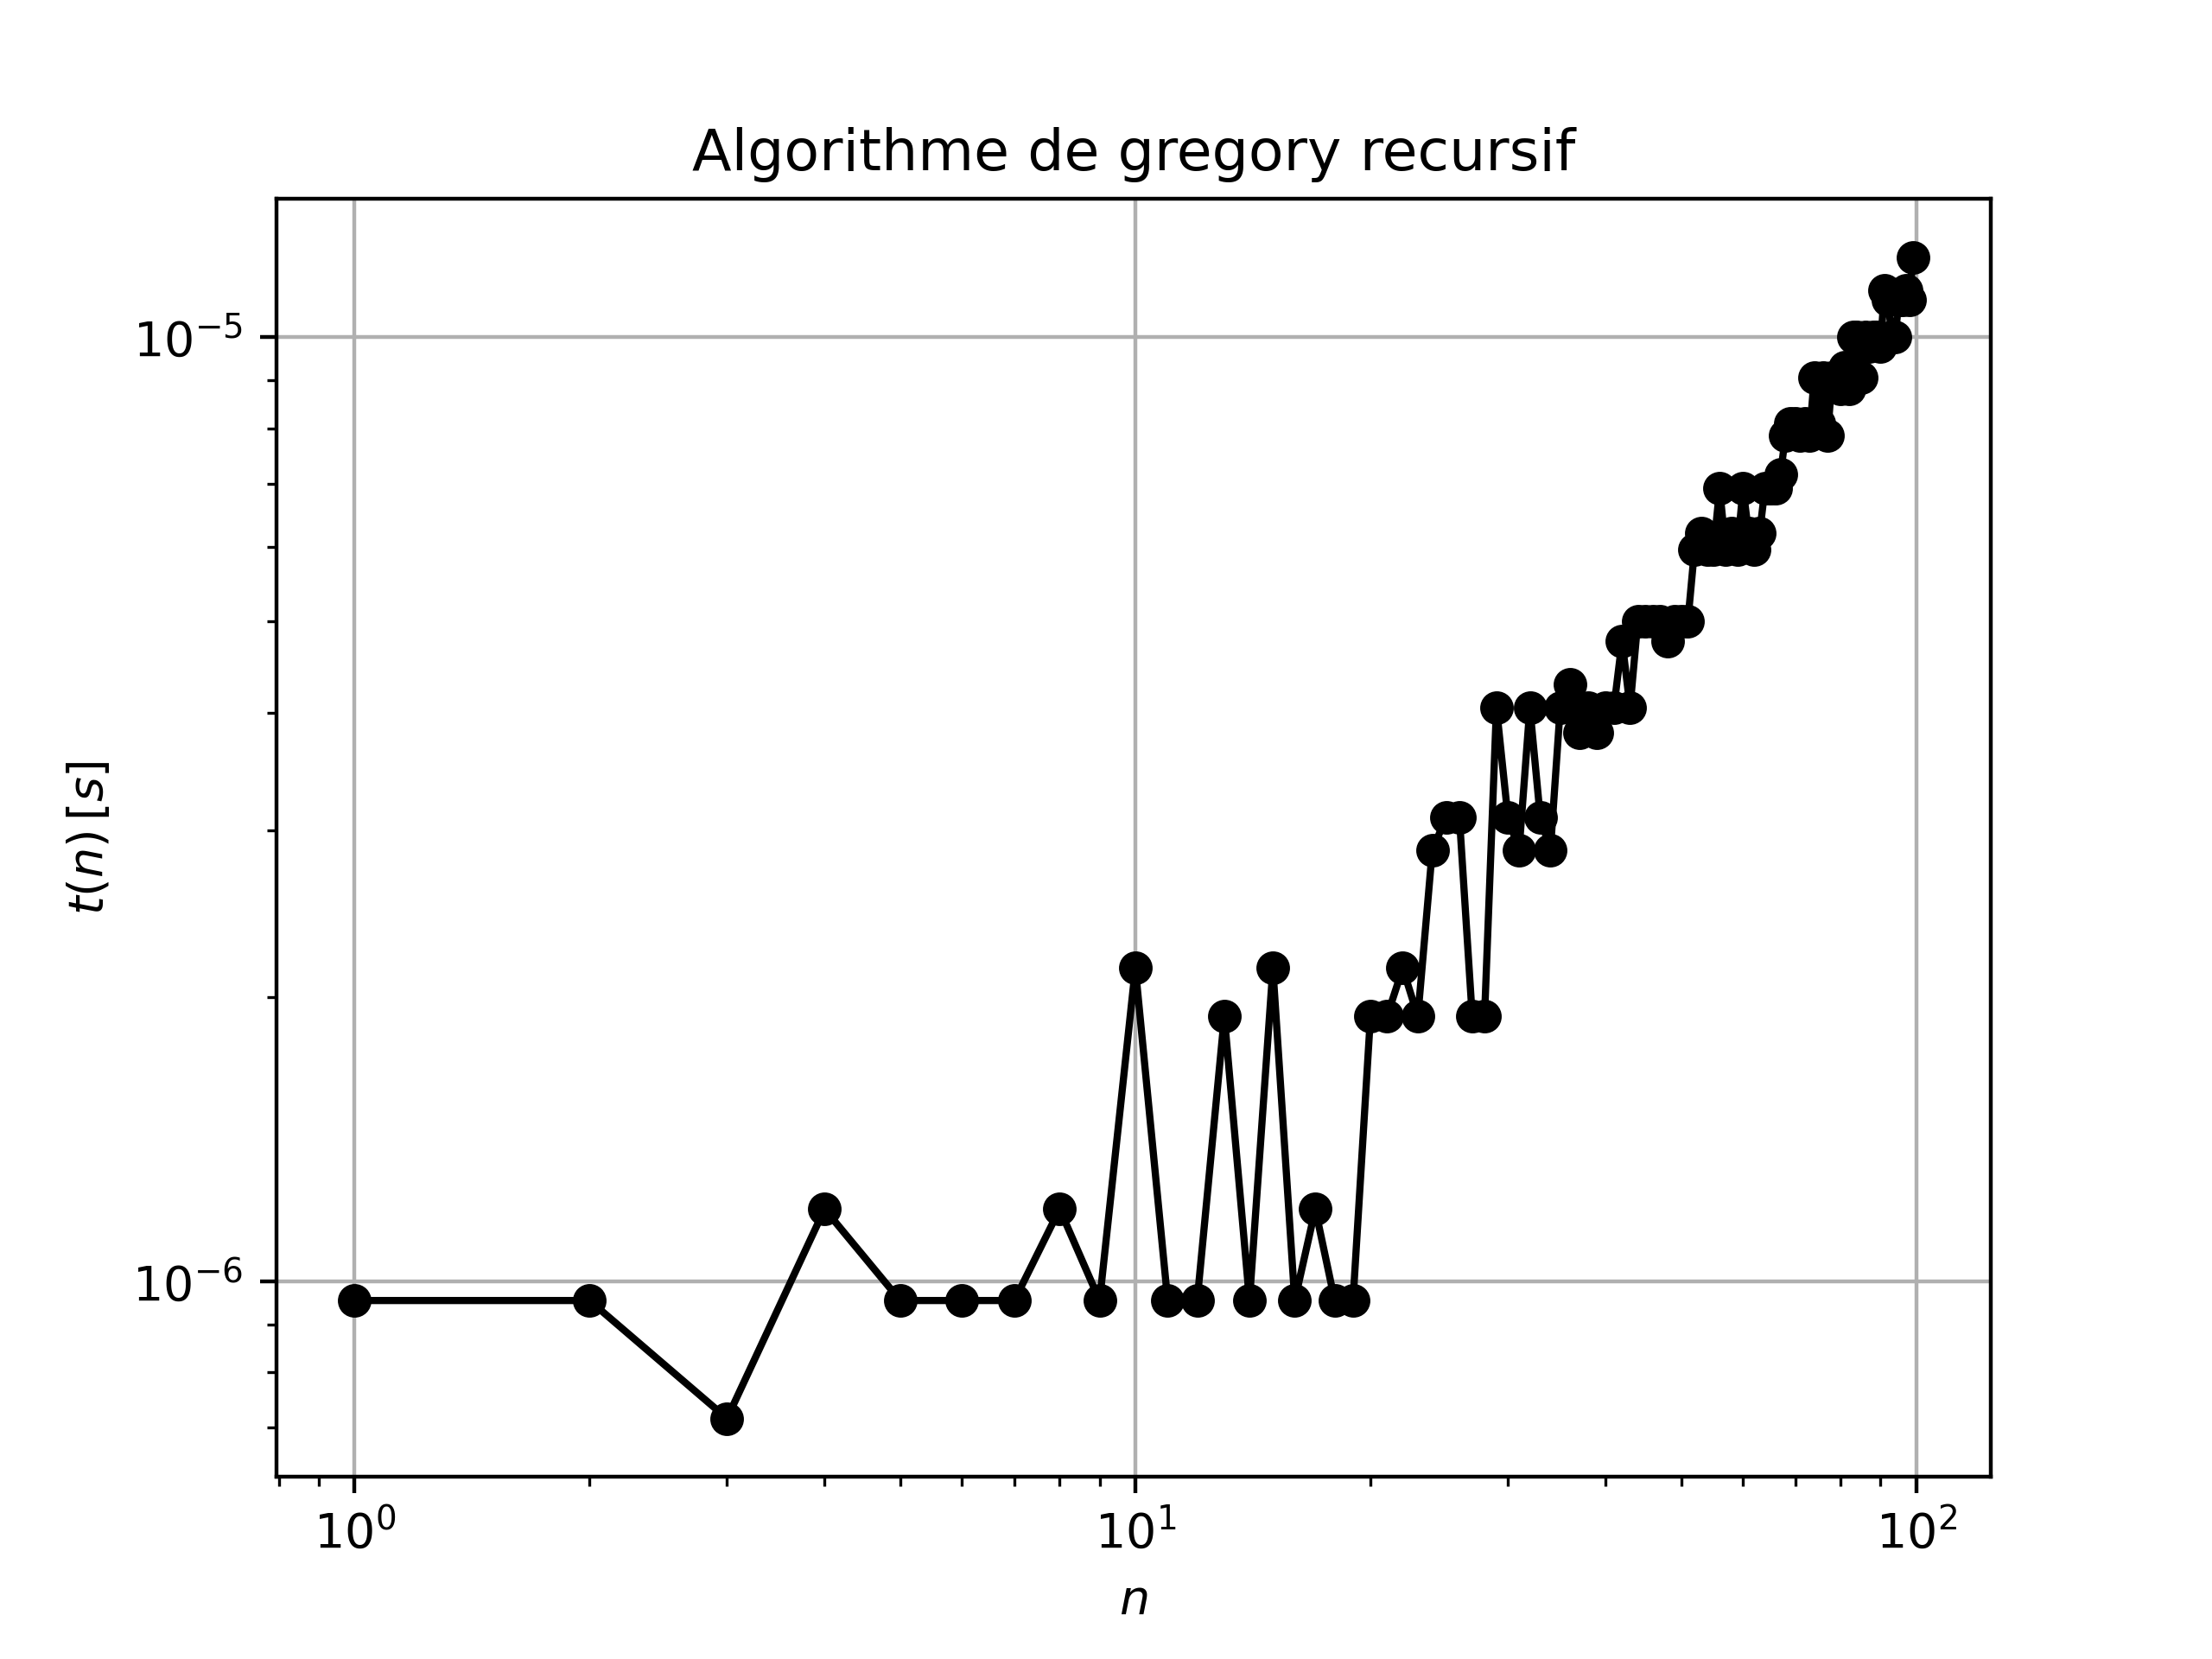
\includegraphics[width=8cm]{./2024/greg-tim.png}
\end{figure}
\clearpage
Une proposition de correction
\lstinputlisting[language=Python]{./2024/exo1.py}
\clearpage
On obtient les figures suivantes
\begin{figure}[htbp]
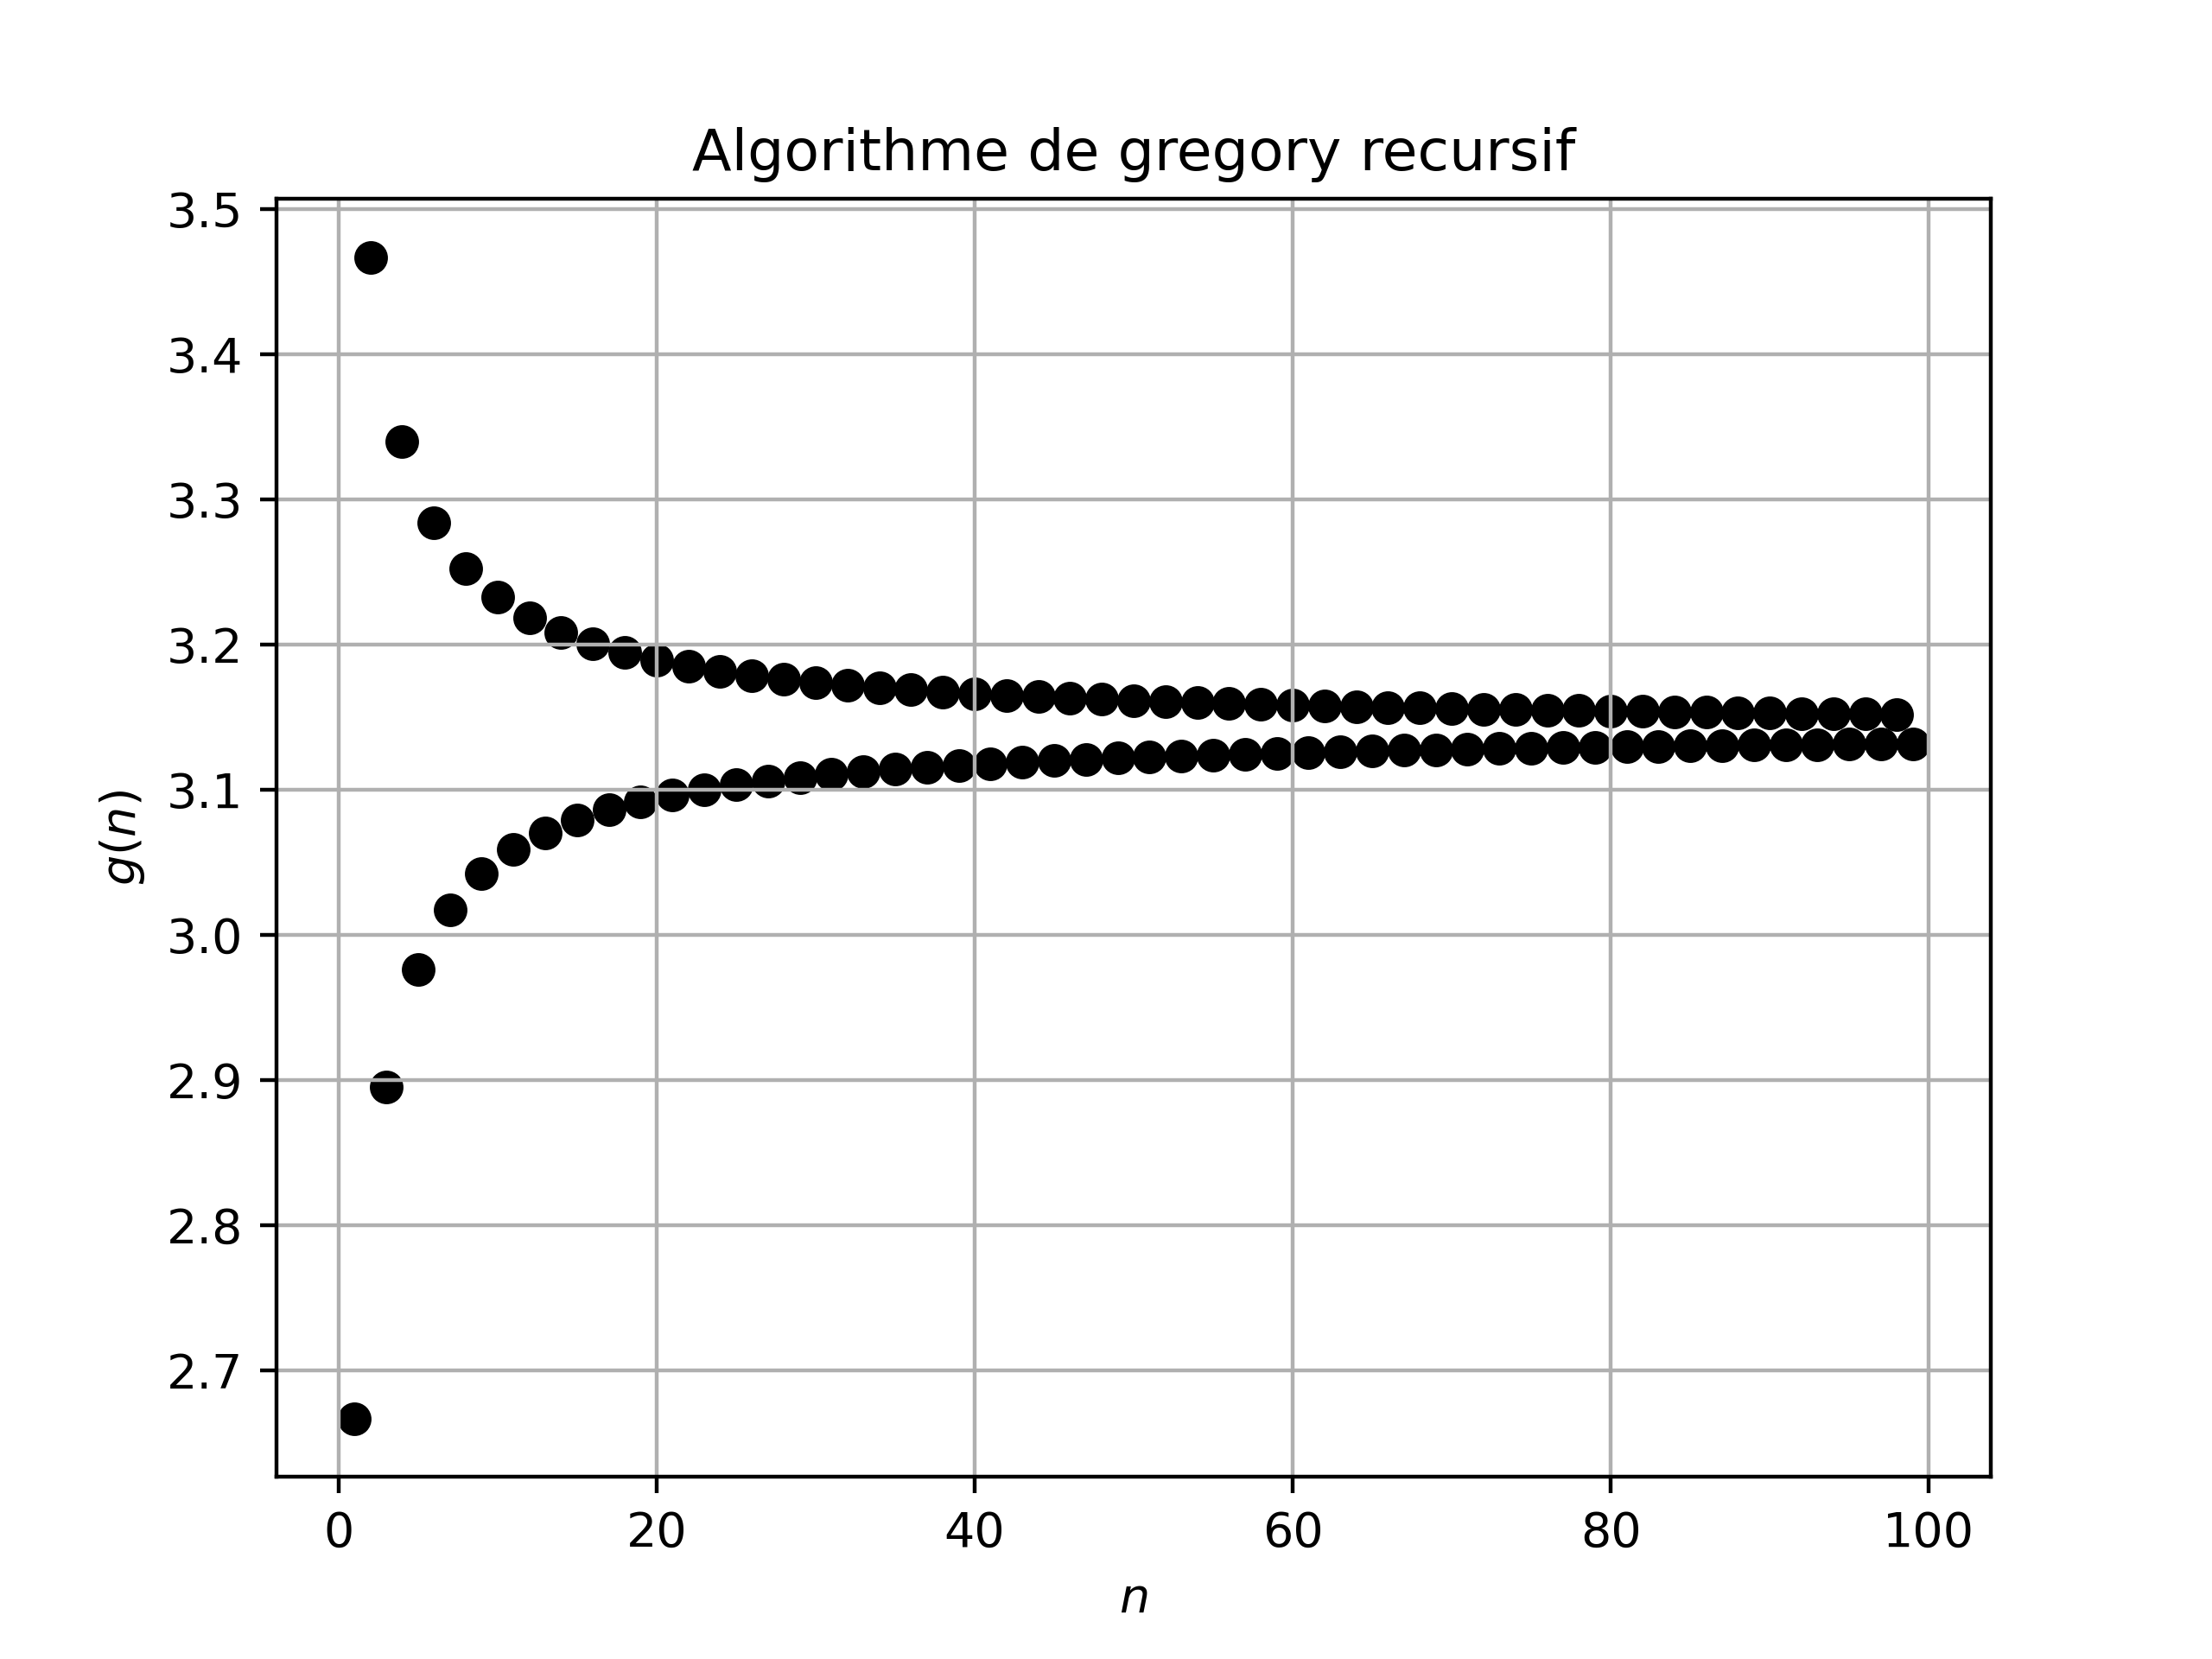
\includegraphics[width=8cm]{./2024/greg-val.png}
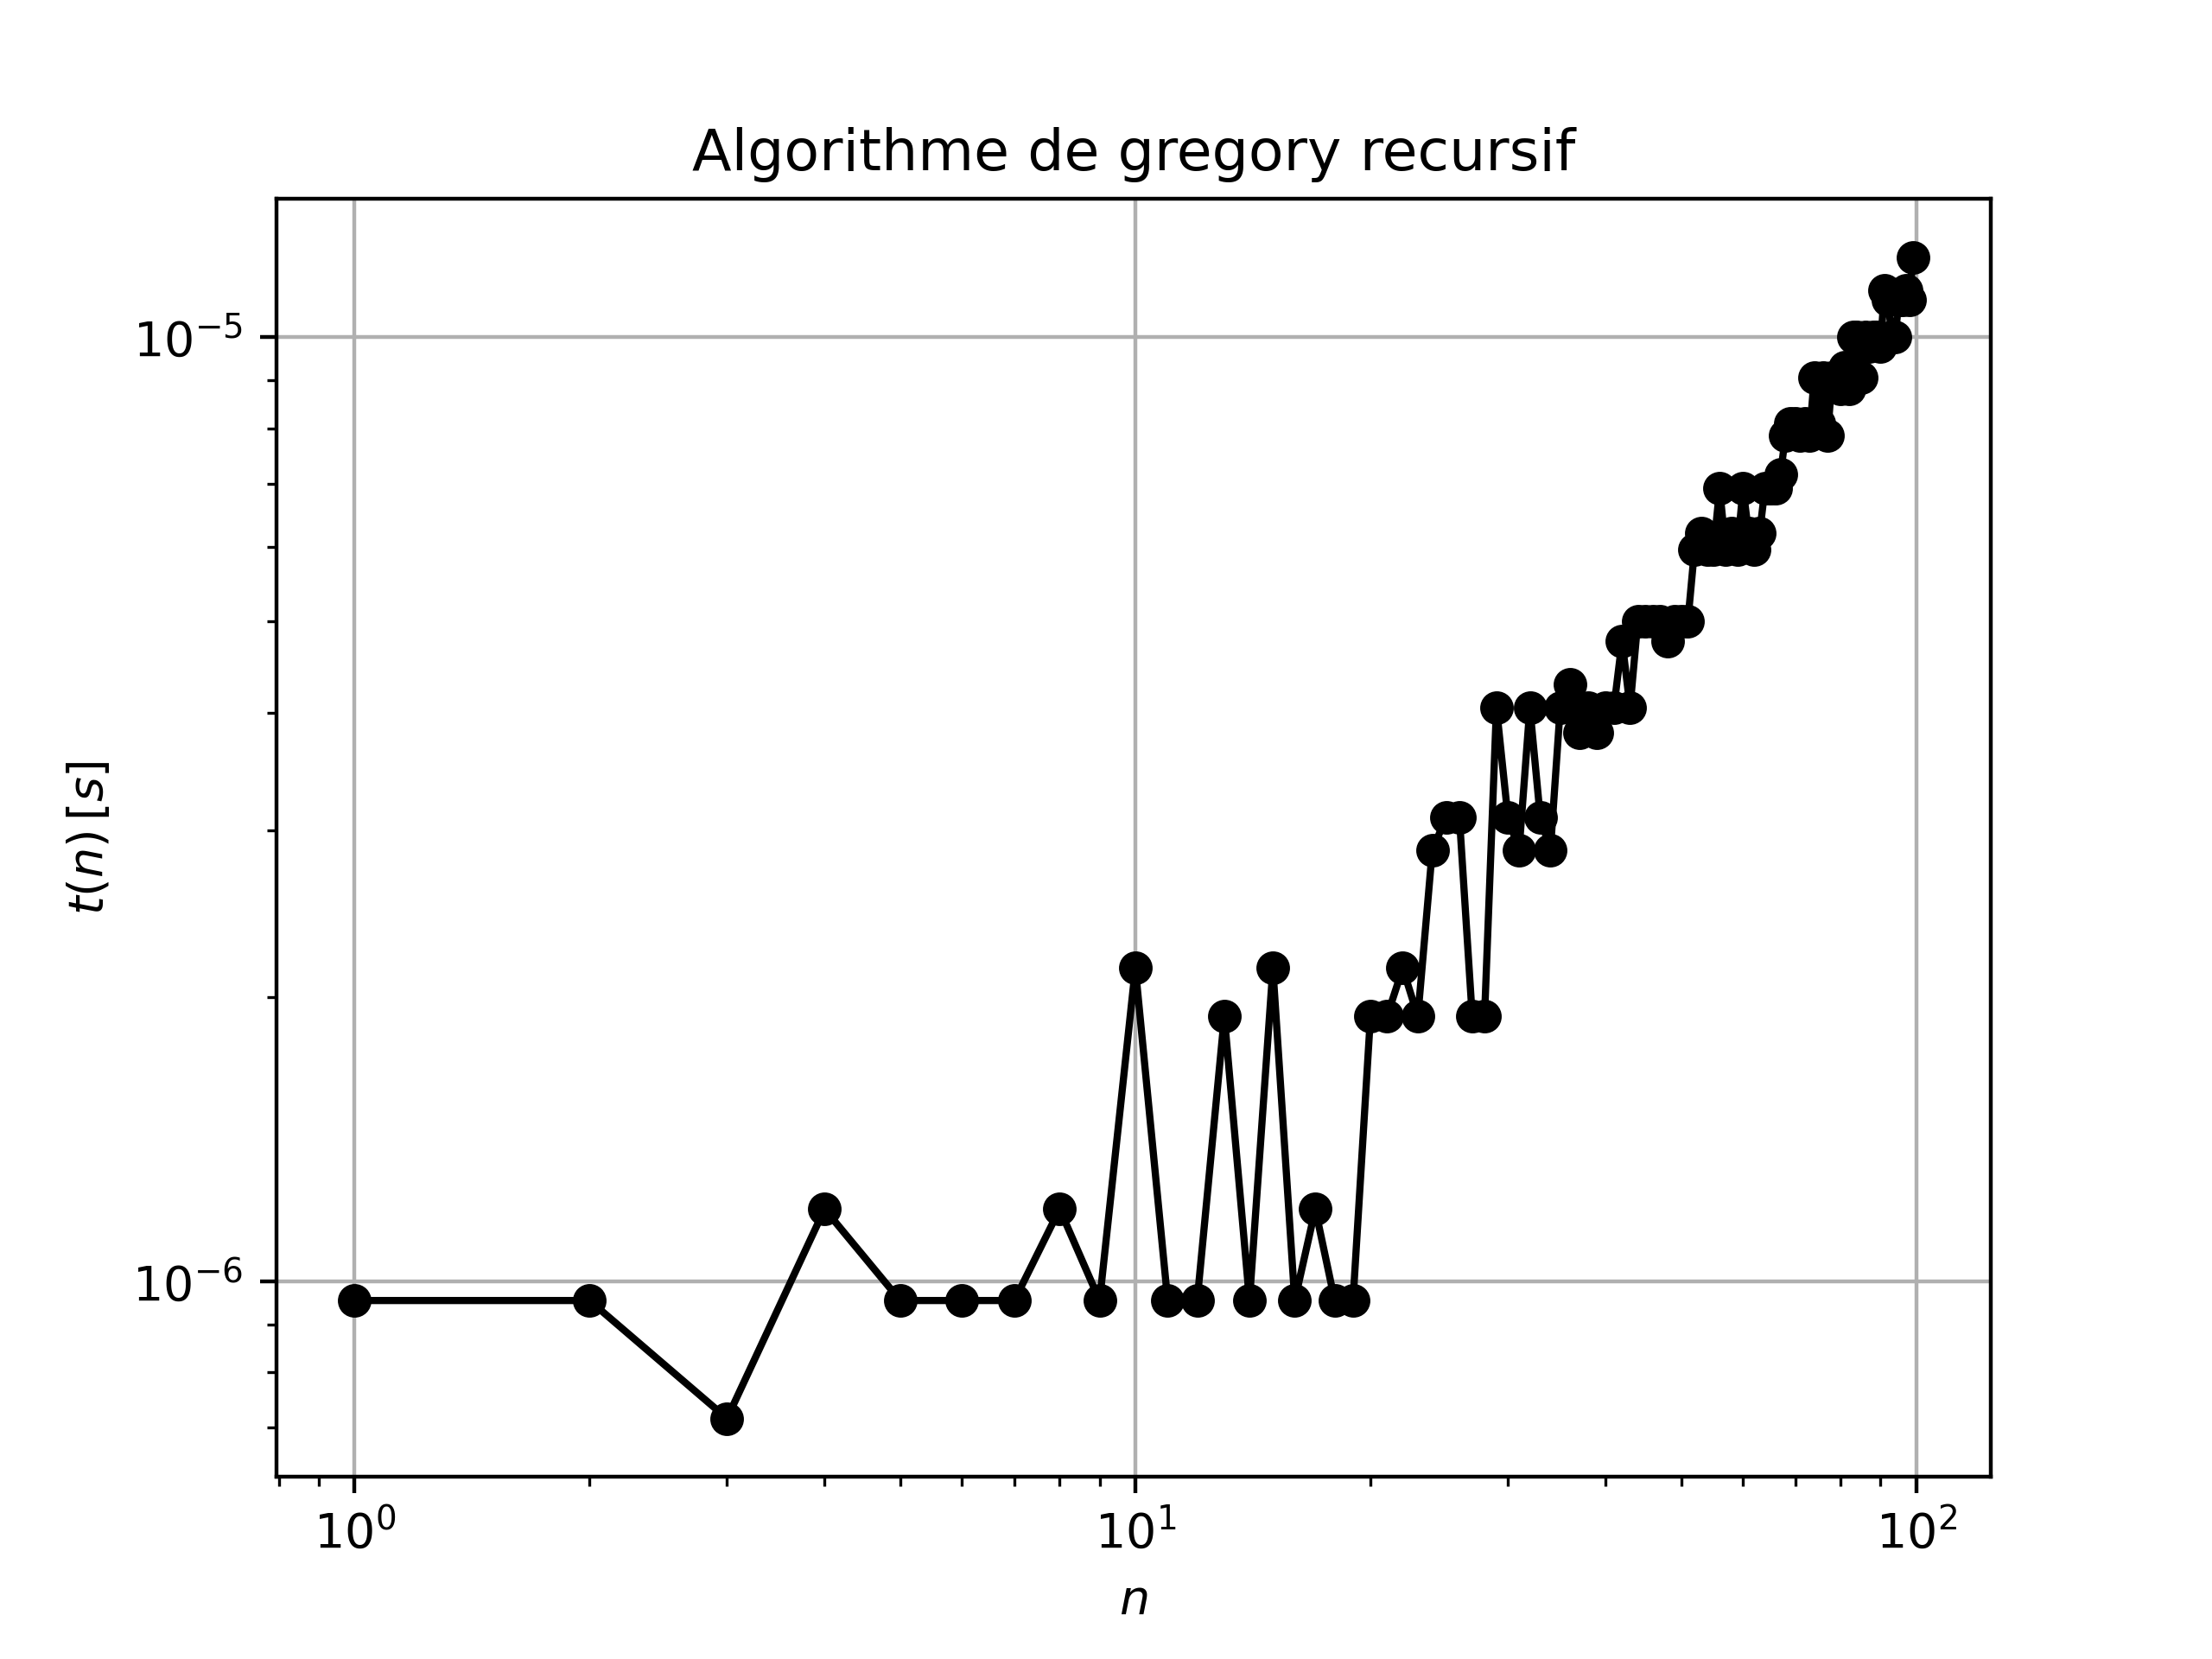
\includegraphics[width=8cm]{./2024/greg-tim.png}
\end{figure}
\begin{figure}[htbp]
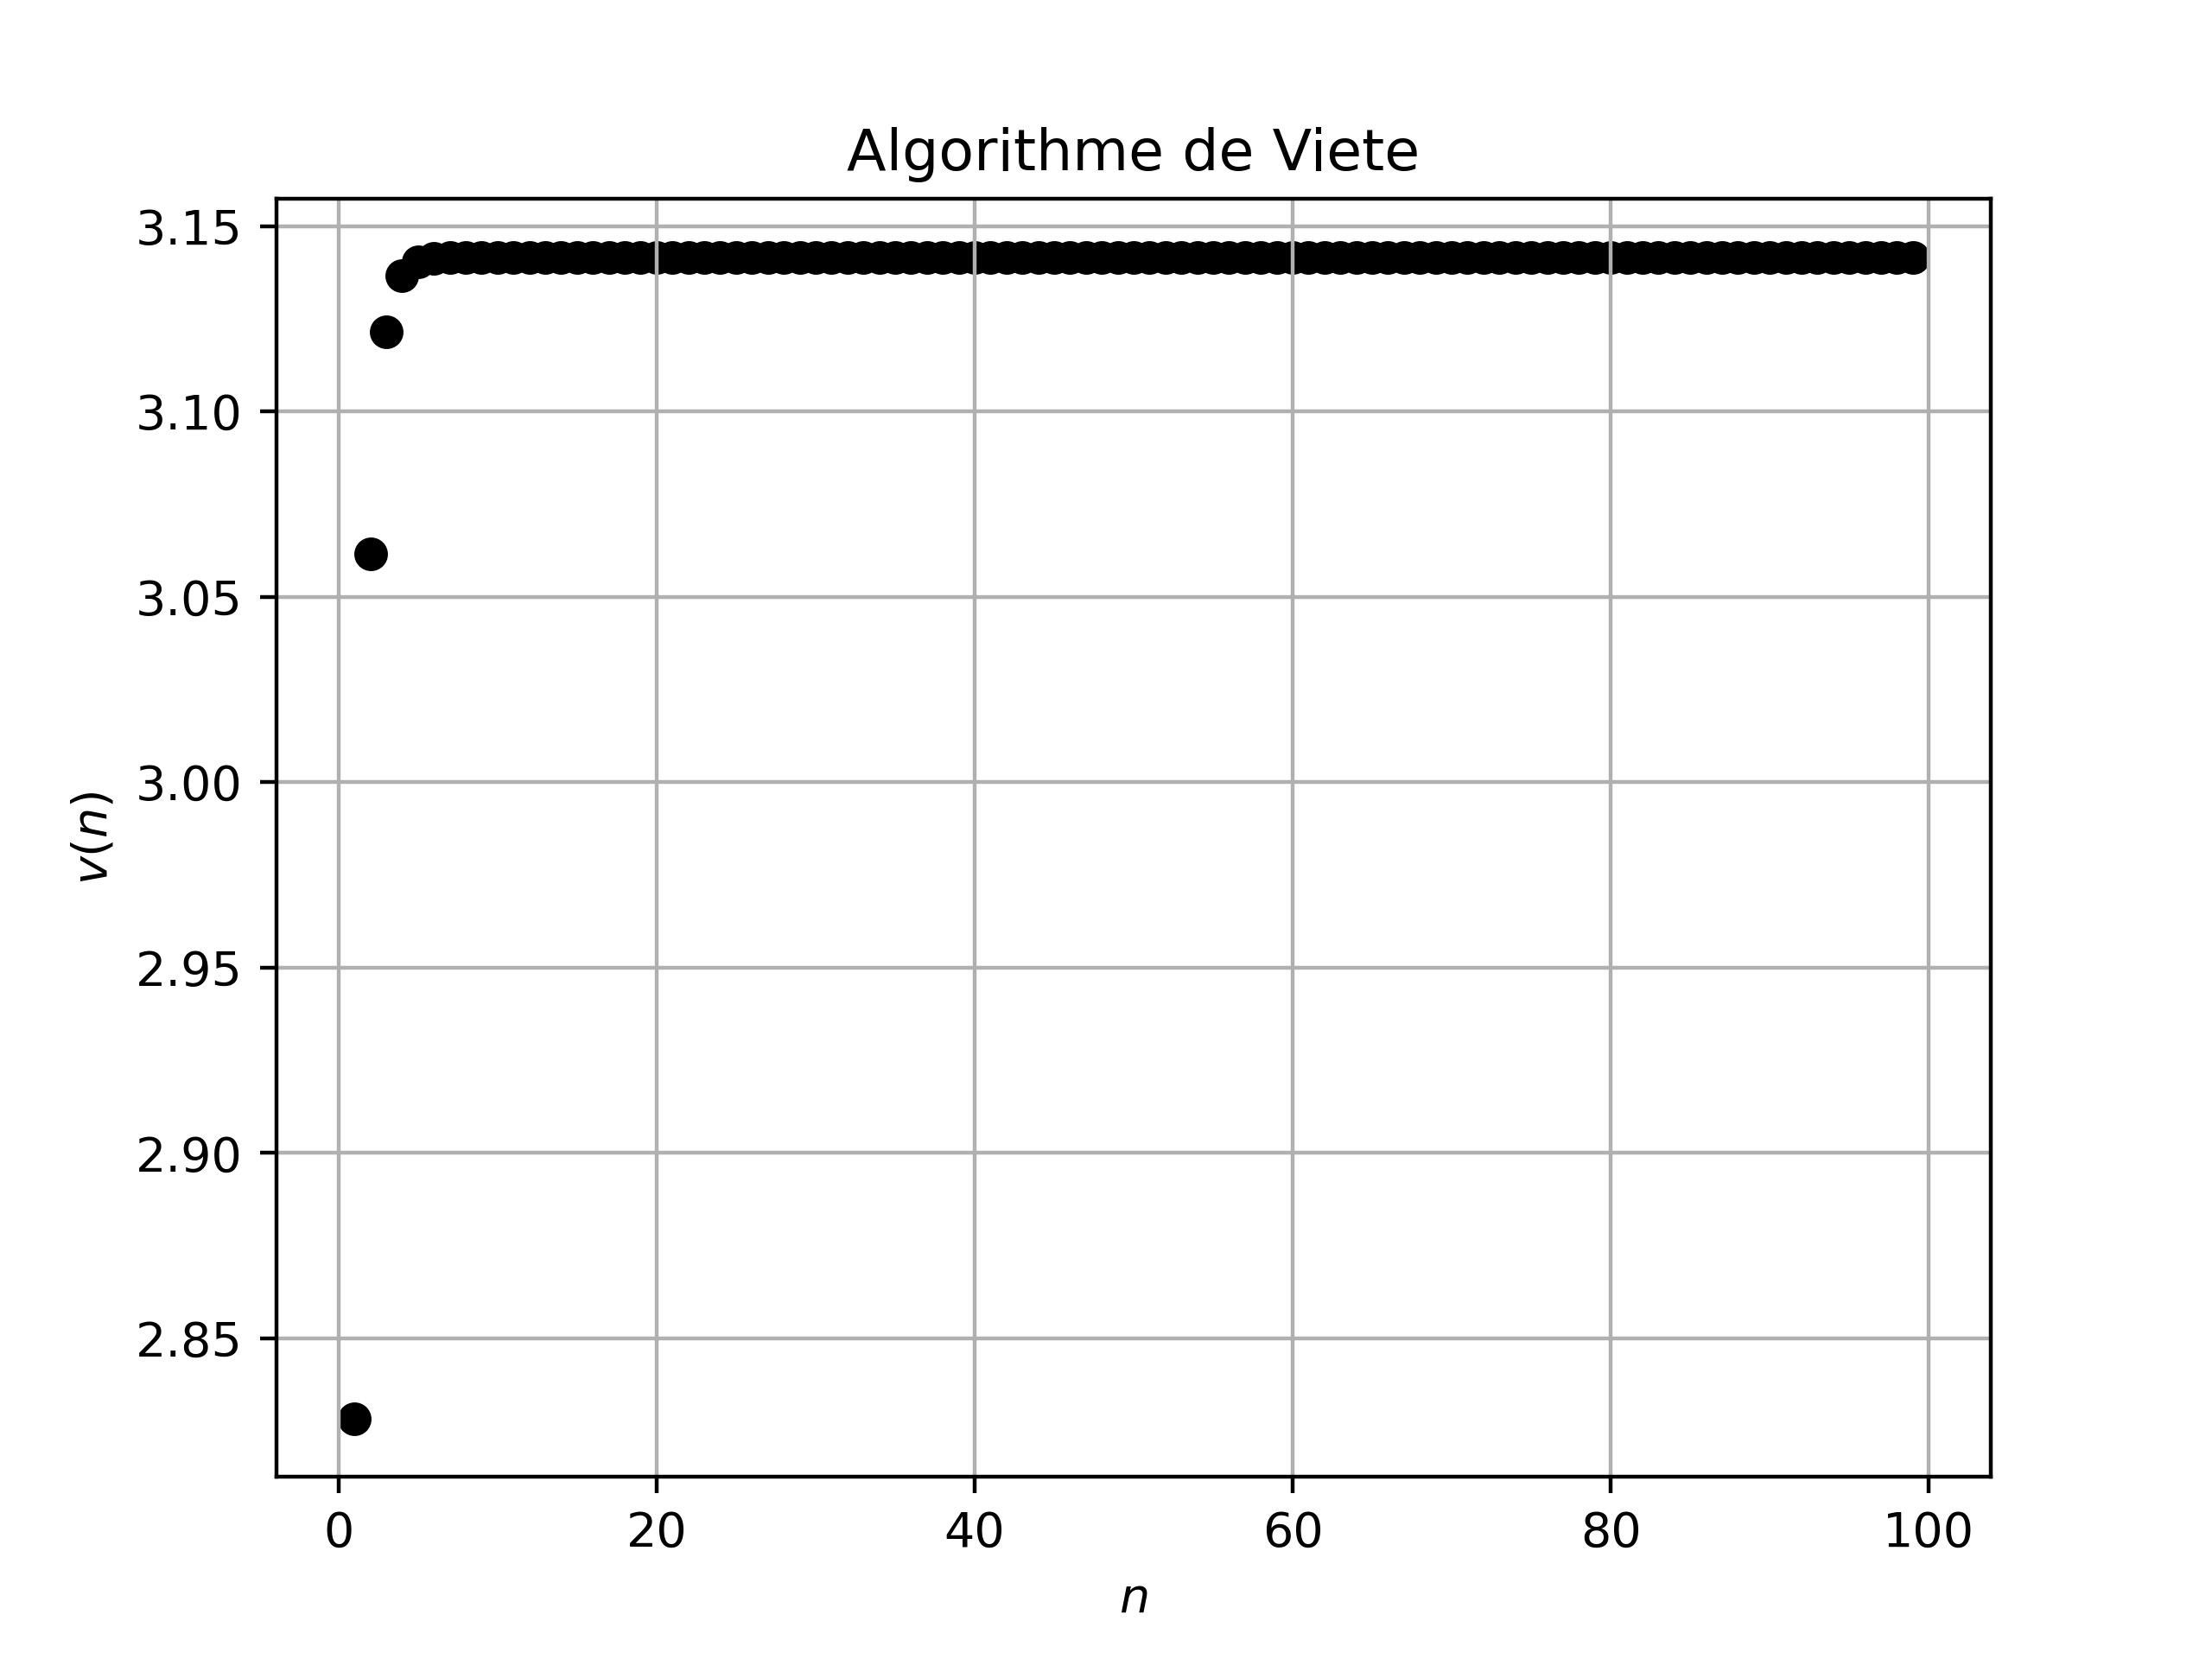
\includegraphics[width=8cm]{./2024/viete-val.png}
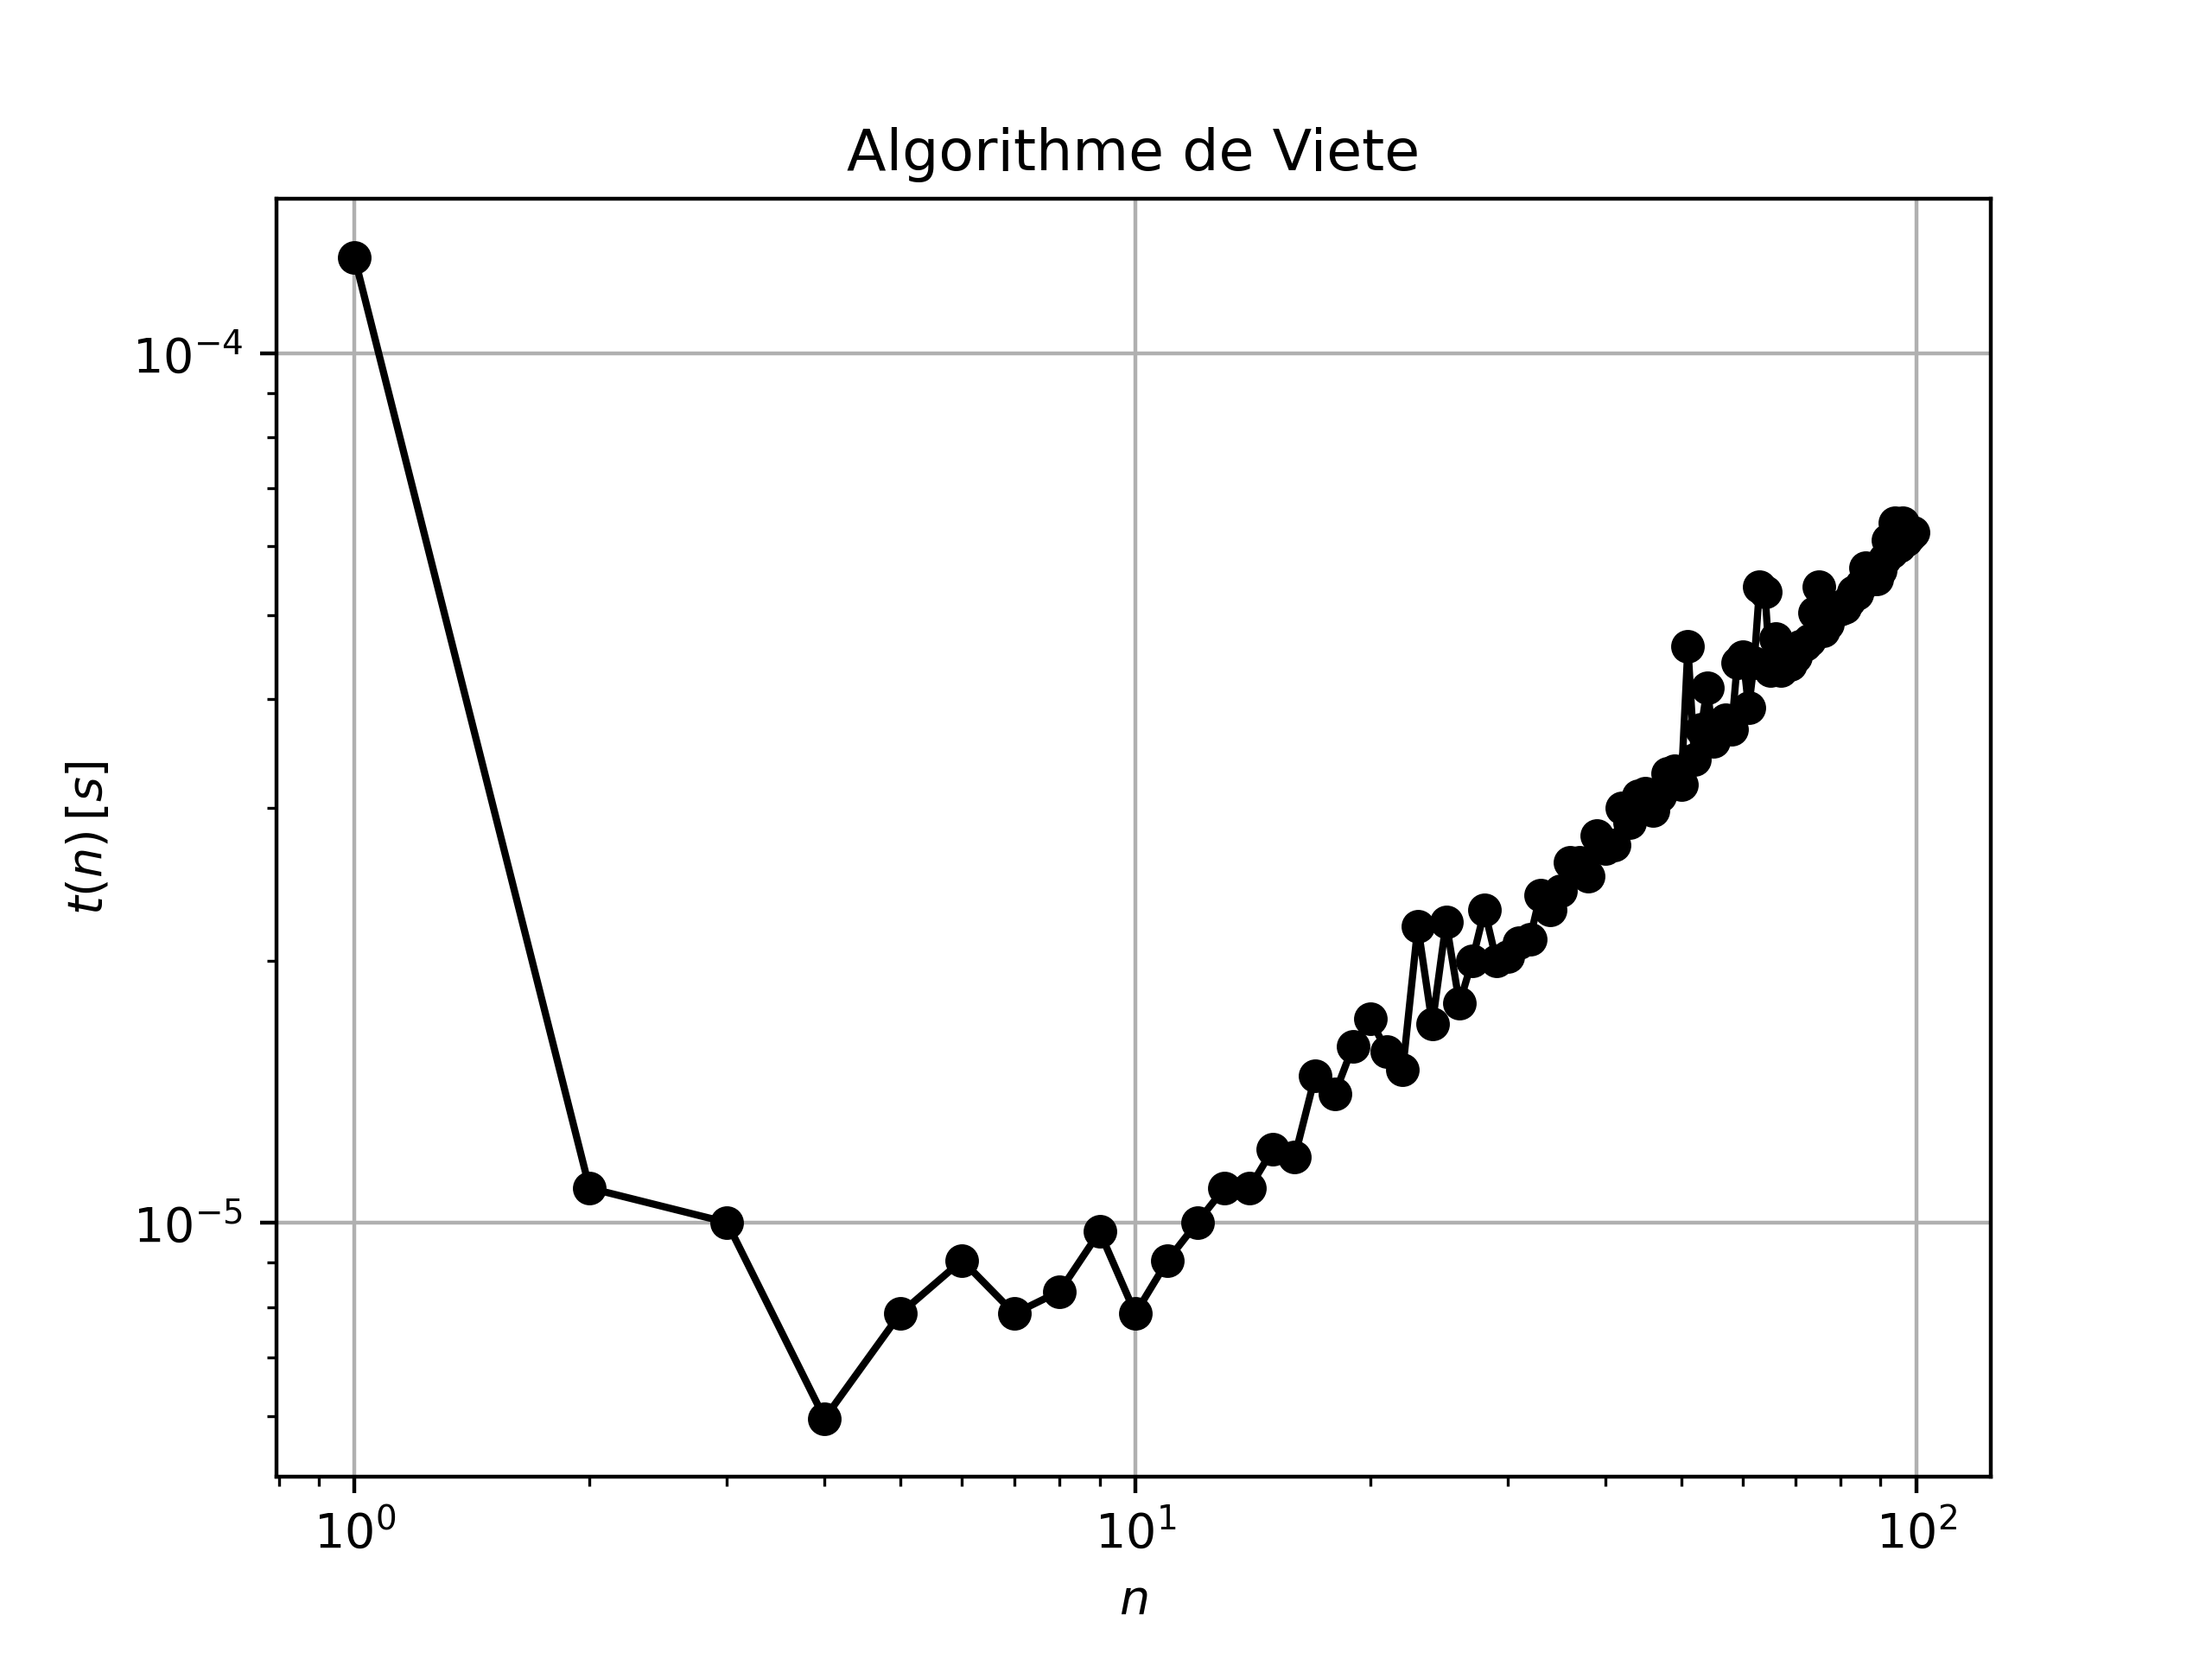
\includegraphics[width=8cm]{./2024/viete-tim.png}
\end{figure}

\clearpage
\subsection{Exercice 2}
\begin{leftbar}
On consid\`ere le calcul de $a^n$ o\`u $a\in\mathbb{R}$ et $n\in\mathbb{N}$.
\begin{enumerate}
\item \'ecrivez une fonction $puiss(a,n)$ calculant $a^n=a\times a\times a\times \ldots \times a$ \`a l'aide de ce produit.  Combien y a-t-il de multiplications? 
\item \'ecrivez une fonction r\'ecursive $puissr(a,n)$ en tirant profit des relations math\'ematiques 
$a^n=(a^{n/2})^2$ si $n$ est pair et $a^n=a\times \left(a^{\frac{n-1}{2}}\right)^2$ si $n$ est impair.  La fonction renverra le triplet $k(n),t(n),a^n$ o\`u $k(n)$ est le nombre d'appels r\'ecursifs, $t(n)$  le temps de calcul de $a^n$ et $a^n$ le r\'esultat de l'op\'erations.  Pour calculer $k(n)$ on d\'efinira une variable global $k$ que l'on initialisera \`a z\'ero \`a l'ext\'erieur de la fonction $puissr$. Dans celle-ci, \`a chaque appel, \'ecrira $k=k+1$ avant l'appel de la fonction  $puissr$. 
\item On prend $a=1.01$ et $n\in\left[1,100\right]$. On demande de mesurer le temps de calcul de chacune de ces deux fonctions en fonction de $n$ et de les repr\'esenter sur un m\^eme graphe comme \`a l'exercice 1.
\item On tracera $k(n)$ en fonction de $n$ sur un autre graphe.
\end{enumerate}
\end{leftbar}
Une proposition de correction
\lstinputlisting[language=Python]{./2024/exo2.py}

On obtient les figures suivantes
\begin{figure}[htbp]
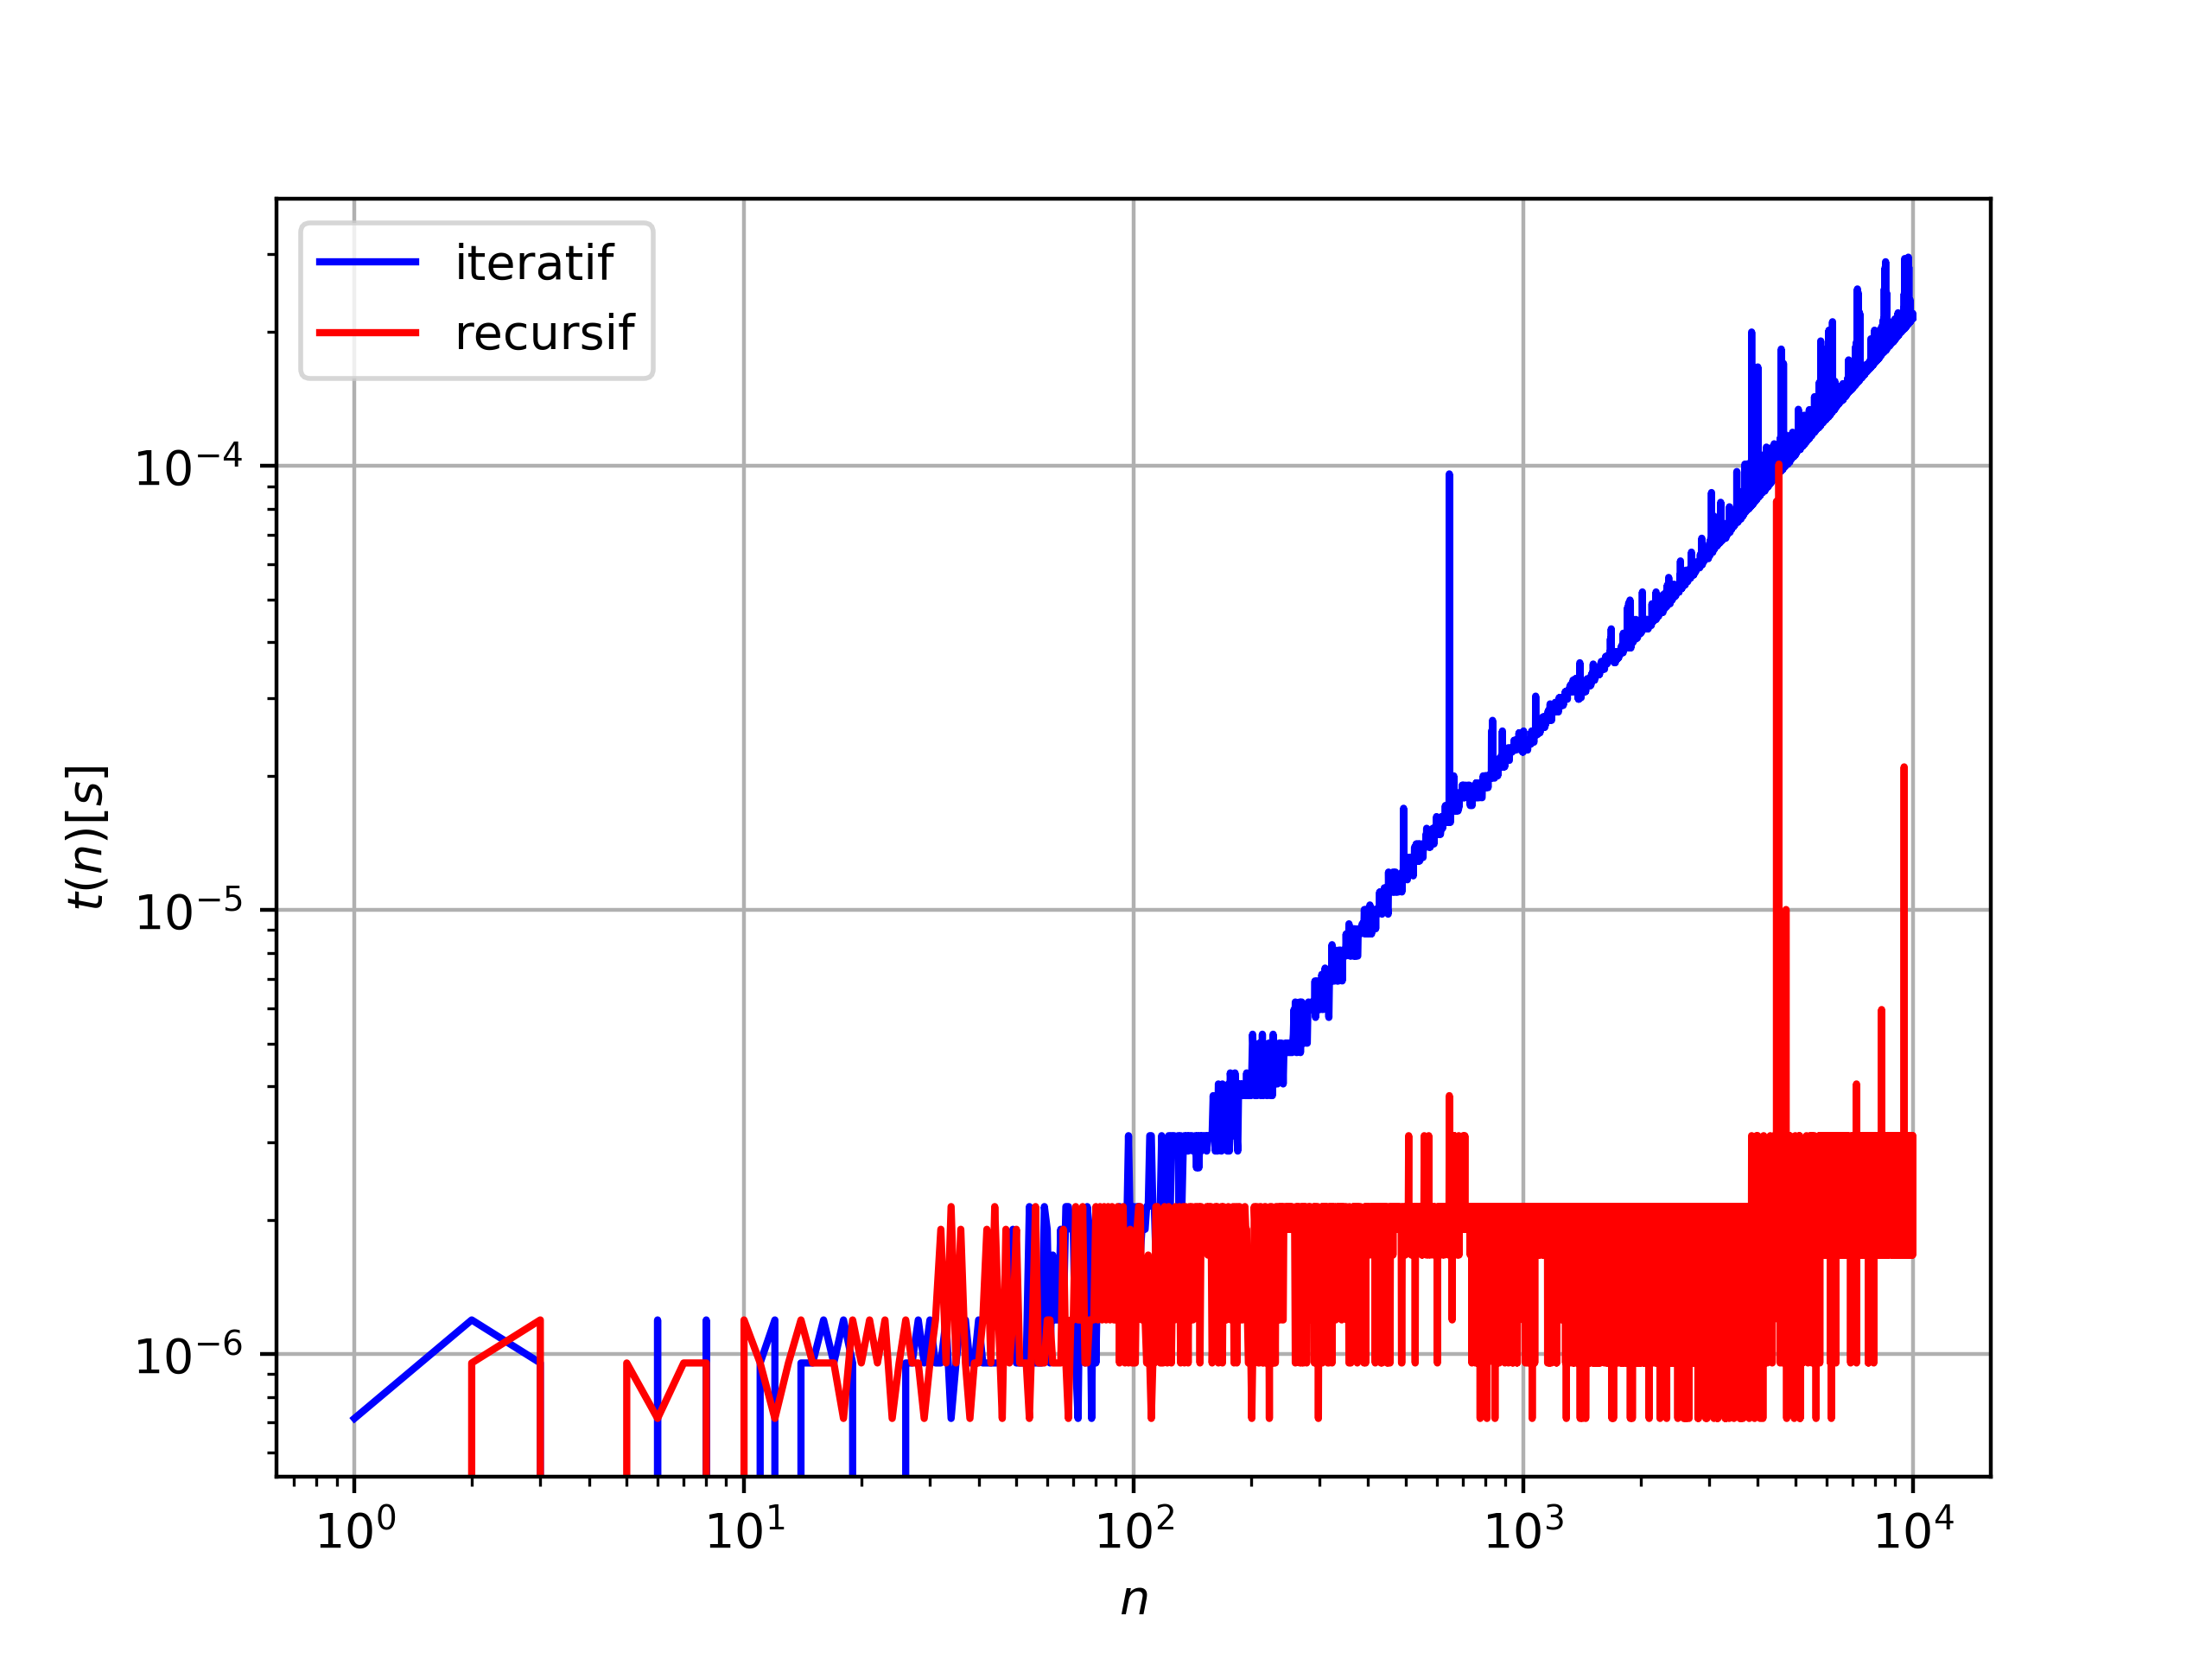
\includegraphics[width=8cm]{./2024/exo2-time.png}
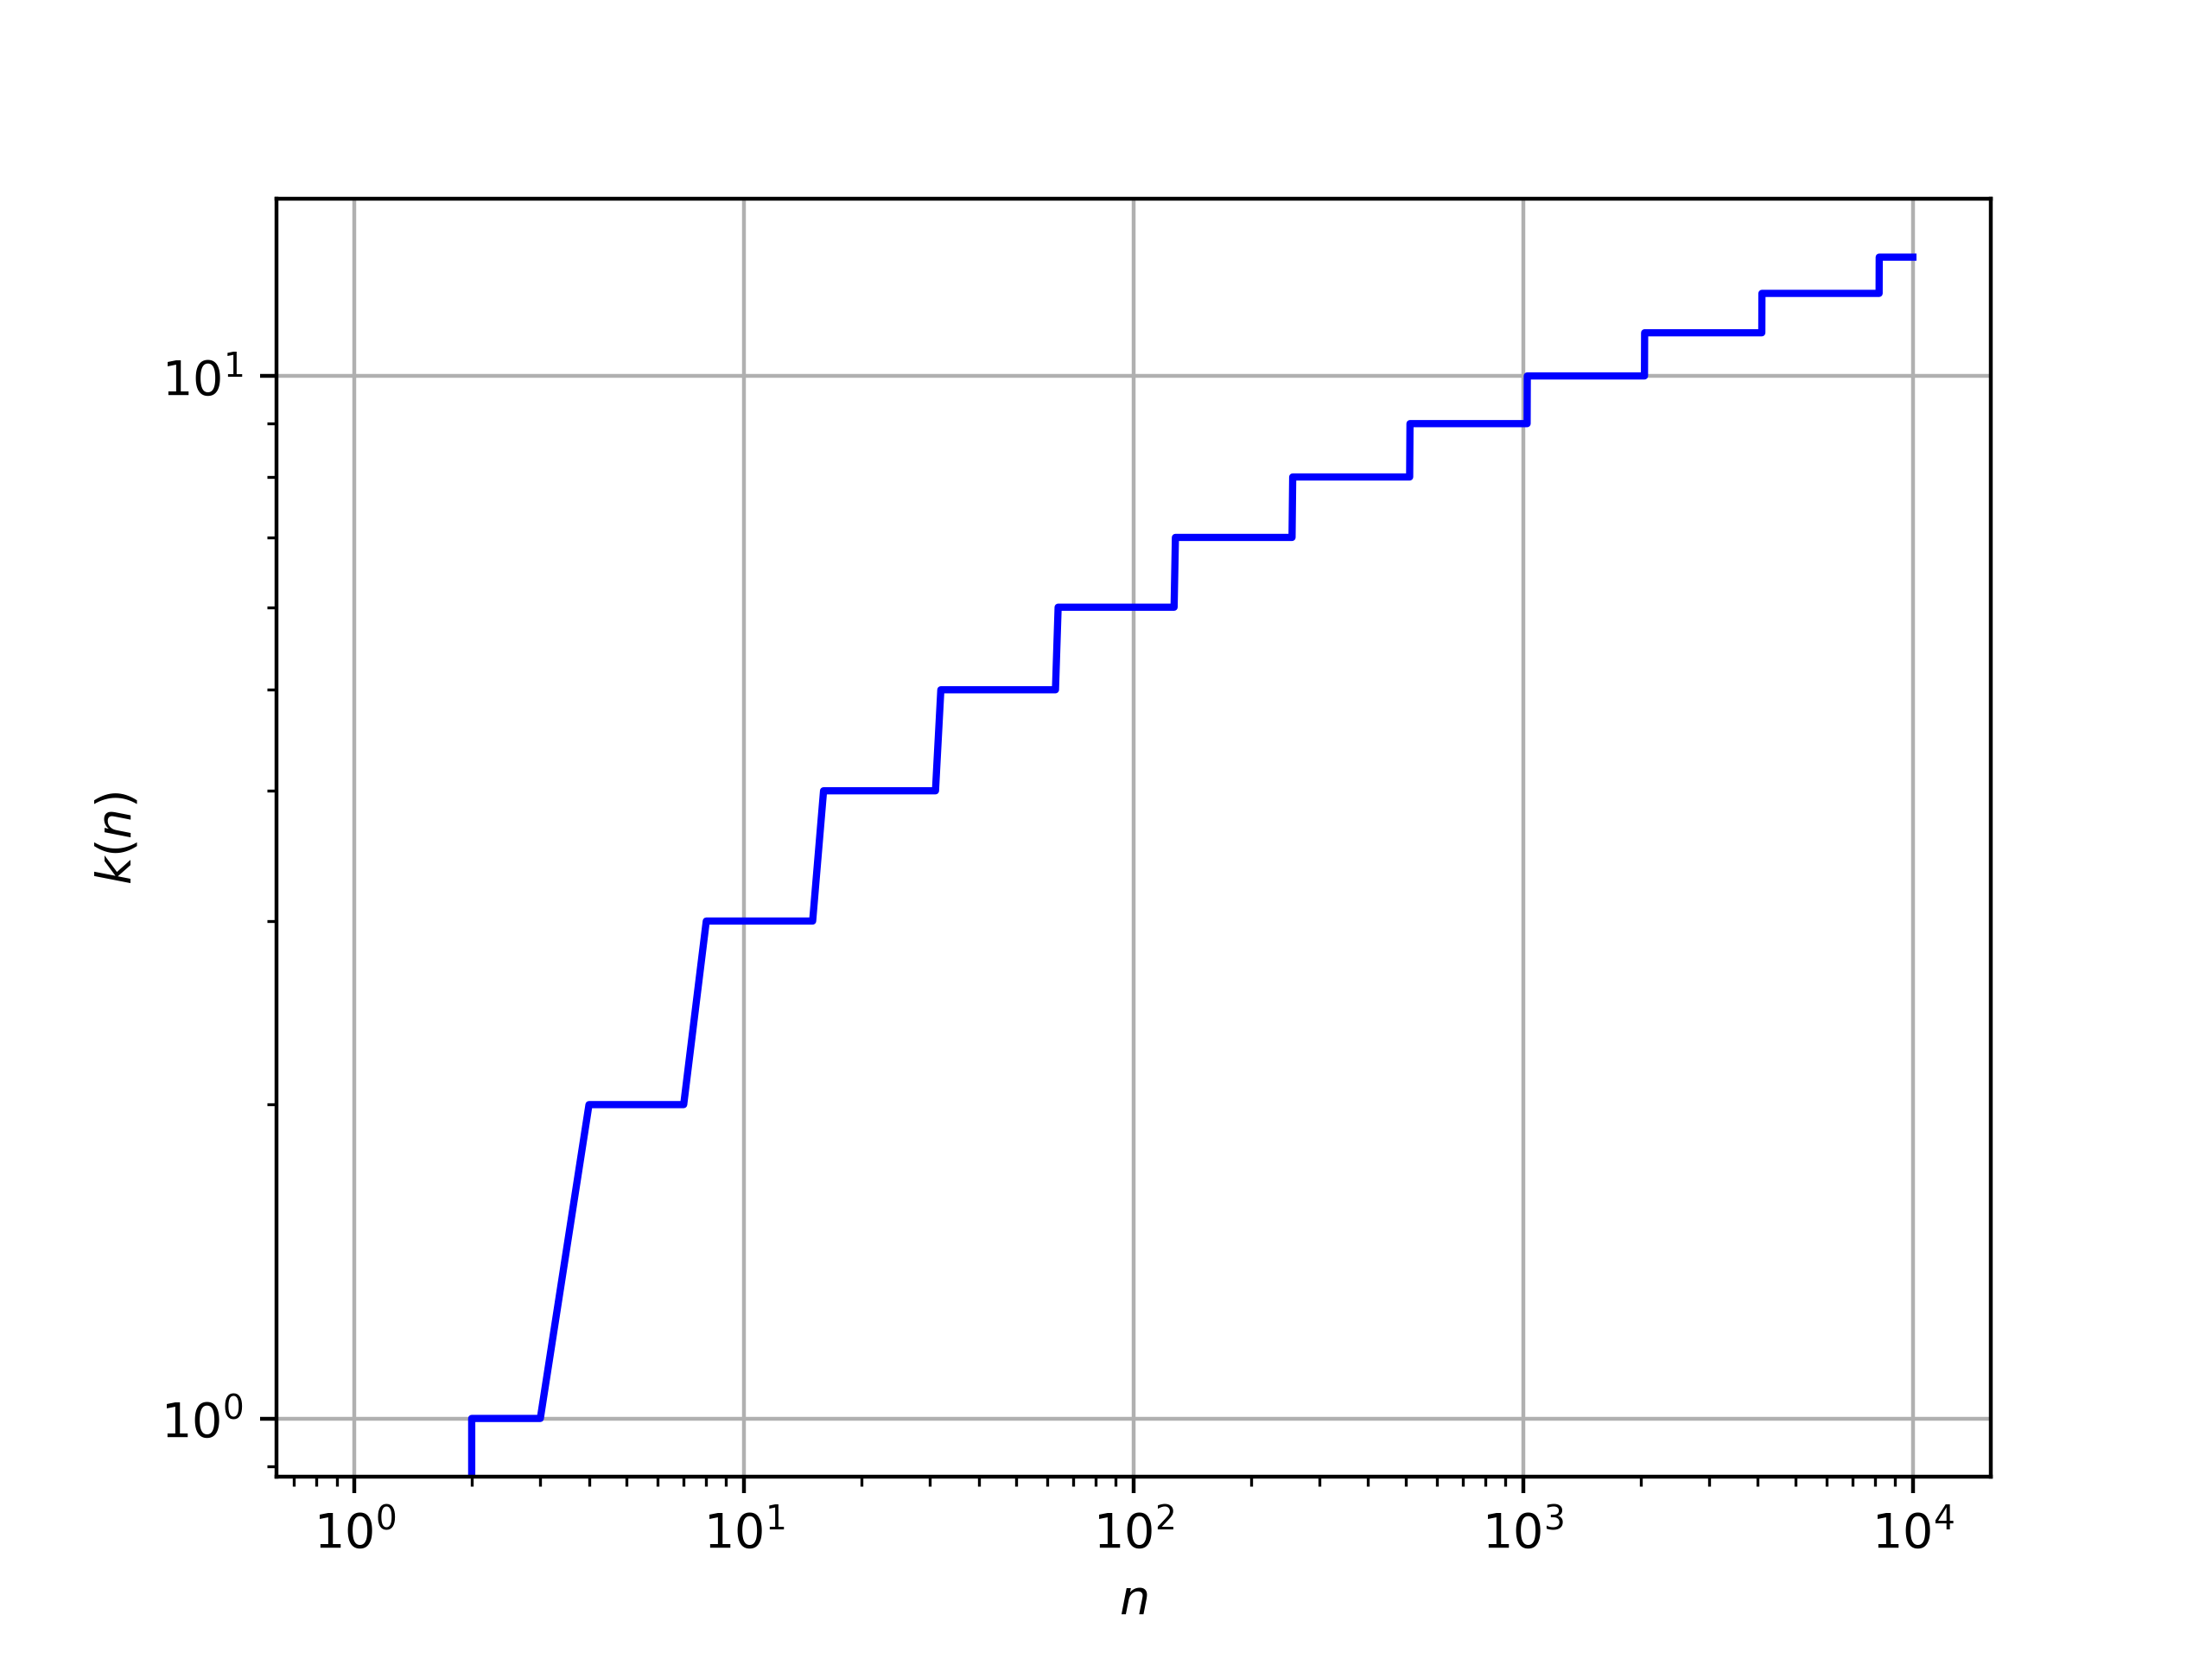
\includegraphics[width=8cm]{./2024/exo2-appel-recursif.png}
\end{figure}


\clearpage
\subsection{Exercice 3}
\begin{leftbar}
On souhaite étudier un  algorithme pour trier les éléments d'un tableau $t$ par packets (trichotomie).
Pour trier les éléments situés entre les indices $i$ et $j$, où $i < j$ du tableau $t$
\begin{enumerate}
\item si les éléments d’indice $i$ et $j$ sont mal placés, on les échange;
\item si il y a au moins trois éléments entre les indices $i$ et $j$
\begin{itemize}
\item on trie les deux premiers tiers du tableau avec cette méthode ;
\item on trie les deux derniers tiers du tableau avec cette méthode ;
\item on trie à nouveau les deux premiers tiers du tableau avec cette m\'ethode
méthode
\end{itemize}
Pour réaliser ce découpage en tiers, on considère l’entier $k=(j – i + 1) // 3$ et les deux entiers $i+k$ et $j-k$. On rappelle que $a//b$ est le qutotient de la division eucildienne de $a$ par $b$. Par exemple $10//7$ renvoie $1$ car $10=1\times 7+3$.
\end{enumerate}
	
\begin{lstlisting}
def Trichotomie(tab, i, j):
	if tab[i] > tab[j]:
		echange(tab, i, j)
	if (j - i) > 1:
		k = (j - i + 1)//3
		Trichotomie(...)
		Trichotomie(...)
		Trichotomie(...)
\end{lstlisting} 

\begin{enumerate}
\item Écrire la fonction echange(tab, i, j) qui prend en arguments une liste
Python tab et deux indices $i$, $j$ , et réalise sur place l’échange des valeurs
dans $tab$ à ces indices. La fonction ne renvoie rien.
\item Compléter les trois dernières lignes de la fonction Trichotomie(...) 
\item Justifier si l'algorithme est r\'ecursif ou it\'eratif.
\item V\'erfier que le code fonctionne avec le tableau $A = [5, 6, 4, 2, 3, 1]$. L'appel est Trichotomie(A,0,5). Afficher les valeurs prises par la variable $k$.
\end{enumerate}
\end{leftbar}

\begin{figure}[htbp]
\begin{center}
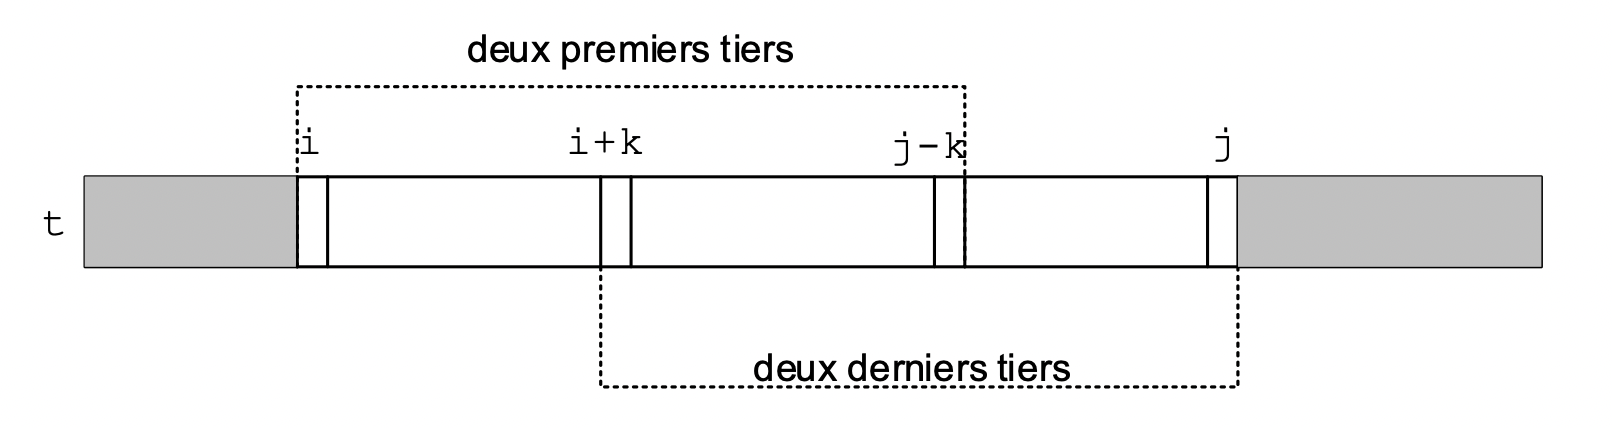
\includegraphics[width=16cm]{./2024/trichotomie.png}
\end{center}
\caption{Localisation des indices $i$, $i+k$, $j-k$ et $j$ du tableau $t$.}
\end{figure}
\clearpage
Une proposition de correction
\lstinputlisting[language=Python]{./2024/exo3.py}
On obtient l'affichage suivant par\`es lancement du script
\begin{verbatim}
avant appel trichotomie: [5, 6, 4, 2, 3, 1]
k = 1
k = 1
k = 1
k = 1
k = 1
k = 1
k = 1
k = 1
k = 1
k = 1
k = 1
k = 1
k = 2
apres appel trichotomie: [1, 2, 3, 4, 5, 6]
\end{verbatim}

\clearpage
\subsection{Exercice 4}
\begin{leftbar}
On consid\`ere une liste $l$ de nombres entiers ou r\'eels ayant $4\times n$ \'el\'ements.
On souhaite \'ecrire une fonction Python $partage(l)$ d\'ecoupant $l$ en 4 sous-listes de taille $n$ not\'ees $l1$, $l2$, $l3$, $l4$ renvoyant
\begin{itemize}
\item les quatre sous-listes $l1$, $l2$, $l3$, $l4$
\item les quatres r\'eels $v1$, $v2$, $v3$ et $v4$ tels que 
\begin{enumerate}
\item $v1$ est la somme des termes de la liste $l1$
\item $v2$ est le produit des termes de la liste $l2$
\item $v3$ est la somme des racines carr\'ees des valeurs absolues des termes de la  liste $l3$
\item $v4$ est la racine carr\'ee de la somme des carr\'es des termes de la liste $l4$
\end{enumerate}
\end{itemize}
\begin{itemize}
\item Si la liste est vide la fonction  $partage(l)$ ne renvoit rien et affiche le message suivant "liste vide". \item Si la liste ne comporte pas un nombre d'\'el\'ements multiple de 4, on affiche un message d'erreur "liste n'ayant pas la bonne taille". Pour obtenir le reste dans la division euclidienne de a par b on \'ecrit $a\%b$.  Par exemple $7\%4$ donne $3$ car $7=1\times 4+3$, donc $7$ n'est pas divisible par $4$.
\end{itemize}
 \end{leftbar}
 
 \clearpage
Une proposition de correction
\lstinputlisting[language=Python]{./2024/exo4.py}
On obtient l'affichage suivant
\begin{verbatim}
17
liste n’ayant pas la bonne taille
0
liste vide
16
\end{verbatim}

\end{document}

